\documentclass{article}
\usepackage[utf8]{inputenc}

\usepackage{graphicx}
\usepackage[margin=0.65in]{geometry}
\usepackage{array}
\usepackage{multirow}
\usepackage{hyperref}
\usepackage{xcolor}
\usepackage{float}
\usepackage{textgreek}

% Unicode字符定义
\DeclareUnicodeCharacter{03B1}{\textalpha}
\DeclareUnicodeCharacter{03B2}{\textbeta}
\DeclareUnicodeCharacter{03B3}{\textgamma}
\DeclareUnicodeCharacter{03B4}{\textdelta}
\DeclareUnicodeCharacter{03C0}{\textpi}

\title{Strategic Intelligence and Deception Capabilities in Large Language Models: A Game-Theoretic Analysis Using Liars Bar}
\author{Team Member: Liguo Lin \\ Date: May 18th, 2025}
\date{}

\usepackage{natbib}
\usepackage{graphicx}

\begin{document}

\maketitle

\begin{abstract}
This study introduces a novel multi-agent strategic game framework, Liars Bar, to evaluate and compare the strategic reasoning and deception capabilities of four prominent Large Language Models (LLMs): ChatGPT, Claude, DeepSeek, and Gemini. Through systematic analysis of 50 game sessions, we assess these models across three critical dimensions: deception capability, survival ability, and decision quality. Our findings reveal distinct strategic profiles: ChatGPT exhibits cautious strategies with high honesty rates, Gemini demonstrates aggressive gameplay with frequent bluffing, DeepSeek balances honesty and deception, while Claude shows adaptable strategy selection. Statistical analyses confirm significant differences between models, with DeepSeek achieving the best overall performance through balanced strategic choices. This research provides insights into LLMs' strategic intelligence, with implications for understanding their reasoning in competitive environments, potential vulnerabilities to manipulation, and future development of more strategically capable AI systems.
\end{abstract}

\line(1,0){550} 
\section{Introduction}
The rapid advancement of Large Language Models (LLMs) has transformed their capabilities from simple text generation to complex reasoning and decision-making \cite{wei2022emergent, bubeck2023sparks}. While these models have demonstrated impressive performance in various domains, their strategic reasoning abilities in competitive environments remain underexplored \cite{gandhi2023}. This research addresses this gap by examining how different LLMs behave in scenarios requiring strategic thinking, deception detection, and adaptive decision-making.

The Liars Bar game provides an ideal testbed for this analysis, as it combines elements of deception, strategic reasoning, and adaptability in a multi-agent environment \cite{aher2023using}. This game framework is particularly well-suited for evaluating LLM strategic intelligence for several key reasons:

\begin{itemize}
    \item \textbf{Isolated Strategic Reasoning:} Unlike games that require domain expertise (e.g., chess) or complex spatial reasoning (e.g., Go), Liars Bar isolates strategic decision-making by focusing on information management, opponent modeling, and risk assessment—capabilities central to strategic intelligence.
    
    \item \textbf{Controllable Complexity:} The game offers sufficient strategic depth to challenge sophisticated models while remaining tractable for systematic analysis, with clearly defined decision points that generate quantifiable metrics.
    
    \item \textbf{Deception Mechanics:} By explicitly incorporating deception as a game mechanic, the framework directly tests LLMs' ability to both generate and detect strategic misinformation—a capability with significant real-world implications.
    
    \item \textbf{Incomplete Information:} The partial observability of game state mirrors real-world strategic scenarios where decisions must be made with limited information, forcing models to reason under uncertainty.
    
    \item \textbf{Multi-agent Dynamics:} The competitive multi-agent setting creates a rich environment for studying how LLMs adapt their strategies in response to others' behaviors, revealing their theory of mind capabilities \cite{ullman2023large}.
\end{itemize}

In this game, players must make strategic decisions about when to play honestly, when to bluff, and when to challenge others' claims, creating a rich context for studying LLMs' strategic capabilities. By analyzing the performance of four prominent LLMs—ChatGPT, Claude, DeepSeek, and Gemini—we gain insights into their different approaches to strategic problems.

Understanding LLM strategic behavior is crucial for several reasons. First, as these models are increasingly deployed in advisory roles across various domains, including business strategy, negotiation, and competitive analysis, their strategic reasoning capabilities directly impact their utility and reliability. Second, analyzing how LLMs handle deception and strategic interactions provides valuable insights into their potential vulnerabilities to manipulation and adversarial inputs. Finally, comparing different models' strategic profiles contributes to our understanding of how architectural differences and training methodologies influence complex reasoning abilities \cite{yang2024rewards}.

This research makes several key contributions:
\begin{itemize}
    \item Introduces a novel multi-agent game framework specifically designed to evaluate LLMs' strategic reasoning and deception capabilities
    \item Provides a comprehensive analysis across three critical dimensions: deception capability, survival ability, and decision quality
    \item Identifies distinct strategic profiles for different LLM architectures, revealing their strengths and limitations in competitive scenarios
    \item Establishes a quantitative methodology for assessing strategic intelligence in AI systems that can be extended to future models and applications
    \item Implements a scalable and robust technical architecture with modular components for game simulation, decision extraction, and multi-dimensional analysis
    \item Develops advanced statistical validation techniques to establish the significance of observed strategic differences between models
    \item Creates novel visualization approaches for complex strategic behaviors, including strategy radar charts and behavioral clustering visualizations
\end{itemize}

Our approach differs fundamentally from previous LLM evaluation methodologies in several critical ways:

\begin{itemize}
    \item \textbf{Beyond Factual Assessment:} While traditional benchmarks like TruthfulQA \cite{lin2022truthfulqa} focus on factual accuracy in isolation, our framework evaluates strategic truthfulness where deception carries both advantages and risks.
    
    \item \textbf{Multi-agent Strategic Interactions:} Unlike single-agent reasoning tasks such as those in the BIG-Bench \cite{kojima2022large}, our approach places LLMs in competitive multi-agent scenarios that require reasoning about others' beliefs and intentions \cite{aher2023using}.
    
    \item \textbf{Quantifiable Strategic Metrics:} In contrast to qualitative assessments of reasoning, we develop fine-grained quantitative metrics that capture specific aspects of strategic intelligence, enabling precise model comparison.
    
    \item \textbf{Adaptive Strategy Analysis:} Beyond static evaluations, our methodology tracks how LLM strategies evolve in response to the game environment and opponents' behaviors, revealing dynamic reasoning capabilities.
    
    \item \textbf{Deception-Aware Evaluation:} Unlike cooperative settings where honesty is optimal, our framework creates contexts where strategic deception may be beneficial, revealing how models balance honesty and deception under incentive structures \cite{evans2021truthful, gandhi2023}.
\end{itemize}

Through this analysis, we aim to advance our understanding of LLMs not just as passive text generators, but as strategic agents capable of sophisticated reasoning in competitive environments.

\section{Related Works}
\subsection{Multi-Agent LLM Systems}
Recent advancements in multi-agent LLM systems have demonstrated the potential of these models in collaborative and competitive environments. \cite{park2023generative} proposed a generative agent framework that simulates human-like behaviors and interactions, enabling the study of emergent social dynamics. Similarly, AutoGen \cite{wu2023autogen} introduces a framework for LLM agents to collaborate through message passing, emphasizing the importance of coordination in multi-agent setups. This coordination capability has been further extended by \cite{gao2023assistgpt}, who introduced AssistGPT as a general multi-modal assistant capable of planning, execution, inspection, and learning across multiple agents. Beyond theoretical frameworks, \cite{qian2024chatdev} demonstrated practical applications by developing communicative agents for complex software development tasks, showing how agent collaboration can solve real-world problems. \cite{talebirad2023multi} and \cite{talebirad2023multiagentcollaborationharnessingpower} have further investigated how intelligent LLM agents can be harnessed for effective multi-agent collaboration, highlighting the importance of communication protocols and role specialization. These frameworks, however, primarily focus on cooperation rather than strategic competition.

\subsection{Strategic Reasoning in LLMs}
The strategic reasoning capabilities of LLMs have been investigated in various contexts. \cite{wang2023voyager} explored how LLMs can be used for planning and strategic exploration in open-ended environments, but did not specifically address competitive settings. This planning ability was further examined by \cite{huang2022language}, who demonstrated LLMs' zero-shot planning capabilities for extracting actionable knowledge in embodied agents. The ReAct framework proposed by \cite{yao2022react} showed how reasoning and acting can be synergistically combined in language models to improve strategic performance, while \cite{shinn2023reflexion} introduced the Reflexion approach where language agents learn through verbal reinforcement, significantly enhancing their strategic reasoning capabilities. The ability to learn from explanations in context was investigated by \cite{ahn2022can}, showing that strategic reasoning can be improved through contextual learning. Our work extends these investigations by specifically focusing on strategic decision-making in competitive, information-limited environments.

\subsection{Game Theory and LLMs}
The intersection of game theory and LLMs represents an emerging area of research. \cite{xu2023exploring} explored how LLMs perform in classical game theory scenarios such as the Prisoner's Dilemma and Ultimatum Game, finding that these models often deviate from game-theoretic optimal strategies. This observation was extended by \cite{akata2023playing}, who systematically studied LLMs' behavior in repeated games, revealing interesting patterns of cooperation and competition emergence. \cite{dafoe2020open} provided a comprehensive framework of open problems in cooperative AI, many of which are applicable to LLM multi-agent systems. Our research builds upon these studies by introducing a more complex game environment that combines elements of deception, strategic adaptation, and risk assessment, offering a more comprehensive evaluation of LLM strategic capabilities.

\subsection{Deception Detection and Generation}
The ability to detect and generate deceptive content is a critical aspect of LLM behavior that has significant ethical implications. \cite{lin2022truthfulqa} developed benchmarks for measuring LLM truthfulness, while \cite{evans2021truthful} explored methods to encourage truthfulness in Large Language Models. The connection between theory of mind capabilities and deception was explored by \cite{ullman2023large}, who demonstrated that LLMs fail on trivial alterations to theory-of-mind tasks, suggesting limitations in their ability to model deceptive scenarios. \cite{gekhman2023trueteacher} introduced TrueTeacher, a method for evaluating factual consistency using LLMs themselves, while the alignment of models with multiple objectives was investigated by \cite{yang2024rewards}. Our work contributes to this area by examining how different LLMs balance honest and deceptive strategies in competitive environments, providing insights into their inherent tendencies toward truthful or deceptive behavior when strategic advantages are at stake.

\subsection{Evaluation Frameworks for LLM Reasoning}
Several frameworks have been proposed to evaluate reasoning capabilities in LLMs. \cite{kojima2022large} explored zero-shot reasoning through chain-of-thought prompting, while \cite{wei2022chain} further developed this approach by showing that chain-of-thought prompting consistently elicits reasoning in large language models. The remarkable ability of LLMs to self-improve their reasoning was demonstrated by \cite{huang2023large}, introducing a new paradigm for assessment focused on learning trajectories rather than static performance. Comprehensive evaluation frameworks such as those proposed by \cite{srivastava2022beyond} have gone beyond simple imitation games to quantify and extrapolate the capabilities of language models across diverse reasoning tasks. The scaling properties of language models and their impact on reasoning capabilities were thoroughly analyzed by \cite{rae2022scaling} in their work on training the Gopher model. However, these frameworks typically focus on standalone reasoning tasks rather than reasoning in interactive, multi-agent environments. Our Liars Bar framework addresses this gap by providing a comprehensive evaluation environment that specifically targets strategic reasoning in competitive settings, offering a new perspective on LLM capabilities beyond traditional benchmarks.

\section{Methodology}
\subsection{Game Design: Liars Bar}
The Liars Bar game serves as our strategic decision-making environment to evaluate LLMs' capabilities. This card game combines elements of deception, strategic reasoning, and psychological gameplay, creating a complex environment where players must make decisions with incomplete information.

\subsubsection{Game Rules}
The game follows these core rules:
\begin{itemize}
    \item \textbf{Setup:} Four LLM agents participate in the game, each starting with 5 points.
    \item \textbf{Cards:} The deck contains Queens (Q), Kings (K), Aces (A), and Jokers, with a randomly selected target card (Q, K, or A) for each round.
    \item \textbf{Gameplay:} In each turn, a player must claim to play 1-3 cards of the target type.
    \item \textbf{Decision Points:}
        \begin{itemize}
            \item Players can play honestly (using actual target cards) or bluff (using non-target cards)
            \item The next player can either accept the play or challenge it
            \item If challenged correctly (the player was bluffing), the challenger gains 1 point and the bluffer loses 1 point
            \item If challenged incorrectly (the player was honest), the challenger loses 1 point
        \end{itemize}
    \item \textbf{Victory Condition:} A player is eliminated when their points reach zero; the last player standing wins.
\end{itemize}

The complete game flow, including decision points and outcome calculations, is illustrated in Figure \ref{fig:game_flow}.

\begin{figure}[H]
    \centering
    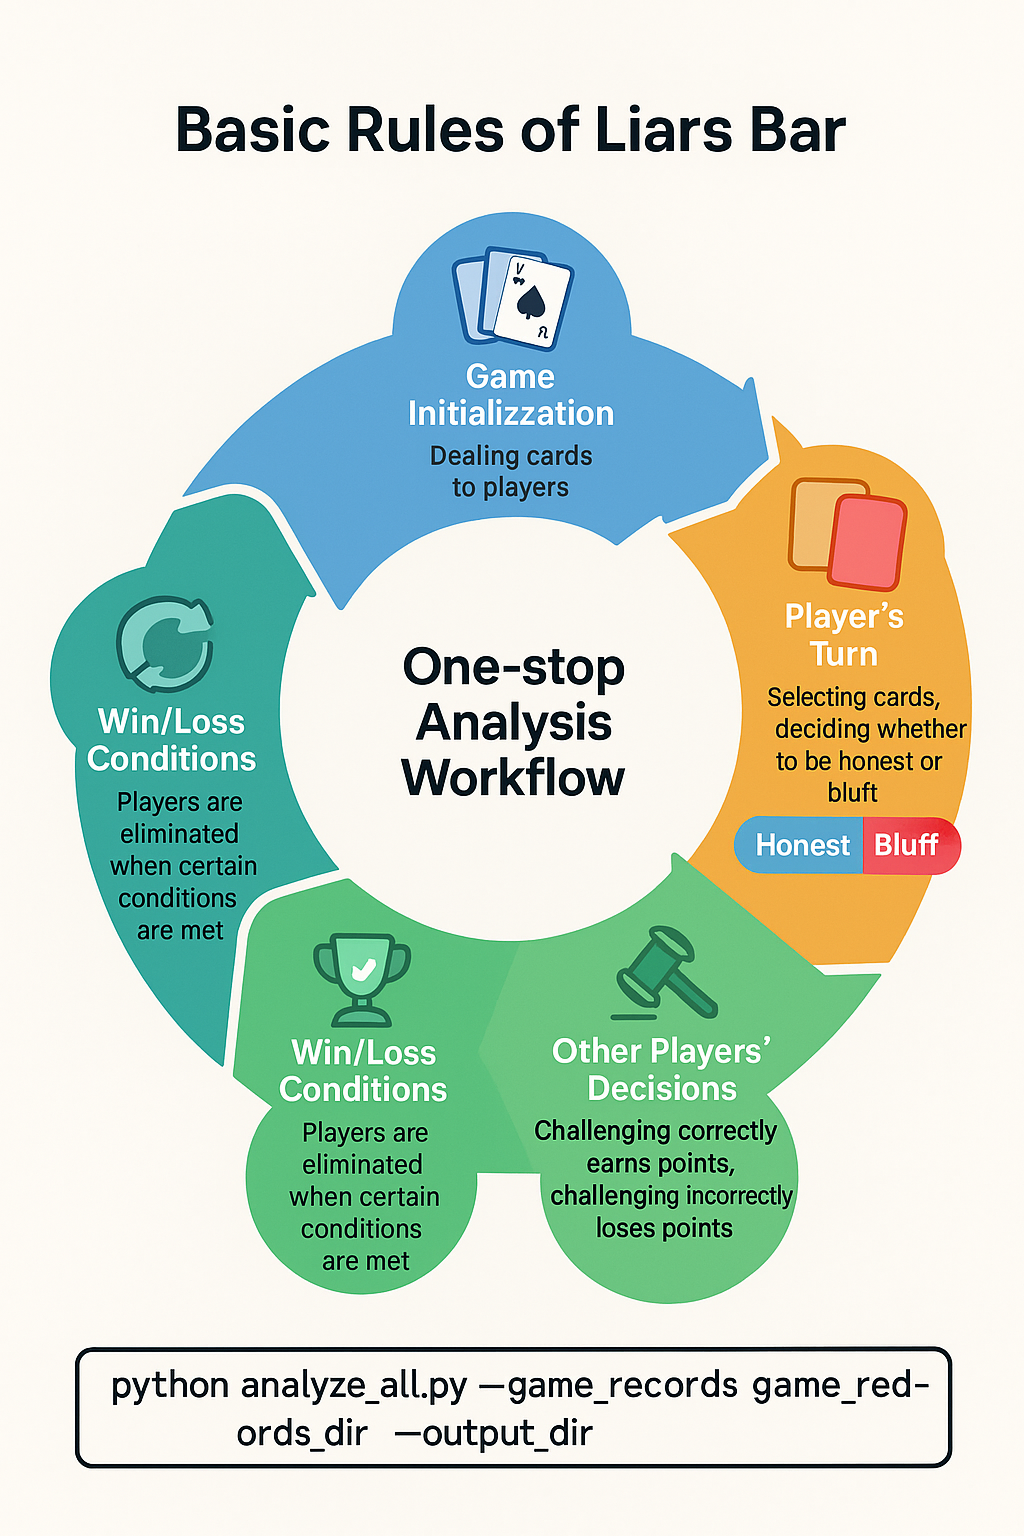
\includegraphics[width=0.8\textwidth]{figures/game_flow.png}
    \caption{Flow chart of the Liars Bar game, illustrating the sequence of decisions and outcomes}
    \label{fig:game_flow}
\end{figure}

\subsubsection{Strategic Elements}
What makes this game particularly suitable for evaluating strategic reasoning is its combination of:
\begin{itemize}
    \item \textbf{Incomplete Information:} Players only see their own cards, creating uncertainty
    \item \textbf{Strategic Depth:} Players must decide when to play honestly, when to bluff, and when to challenge
    \item \textbf{Opponent Modeling:} Success requires adapting to opponents' behavior patterns
    \item \textbf{Risk Management:} Players must balance aggressive and conservative strategies
\end{itemize}

\subsection{System Architecture}
We designed a modular architecture that cleanly separates the game logic from the analysis system, enabling flexible experimentation and comprehensive evaluation, as shown in Figure \ref{fig:system_architecture}.

\subsubsection{Core Game Module}
The game implementation consists of:
\begin{itemize}
    \item \textbf{Game Engine:} Implements the core game mechanics, turn management, and rule enforcement. The engine is built using Python's object-oriented architecture with dedicated classes for Card, Deck, Player, and GameState. State transitions are managed through a finite state machine pattern, ensuring consistent game progression and rule validation at each step. The engine incorporates exception handling mechanisms to manage unexpected model outputs and maintain game integrity.
    
    \item \textbf{Player Interface:} Provides a standardized API for LLM agents to receive game state and submit actions. This interface abstracts model-specific implementation details behind a uniform facade pattern, enabling seamless model substitution without affecting game logic. Each player agent receives partial game information through carefully constructed observation spaces that maintain game-theoretic principles of incomplete information.
    
    \item \textbf{Game Record System:} Captures detailed logs of all game events, player decisions, and outcomes. The system uses JSON-based serialization to store structured records with timestamps, game states, player actions, and decision contexts. This enables comprehensive post-game analysis while maintaining the ability to reconstruct and visualize any game state from the recorded data.
\end{itemize}

\subsubsection{LLM Agent Implementation}
Each LLM agent is implemented with:
\begin{itemize}
    \item \textbf{Model Interface:} Unified API calls to different LLM services using asynchronous communication patterns and robust error handling. Rate limiting and retry logic ensure system resilience against API failures, while a token optimization system minimizes API costs. The interface supports multiple model providers, including OpenAI (ChatGPT), Anthropic (Claude), Deepseek, and Google (Gemini), with adaptive prompt formatting for each service.
    
    \item \textbf{Decision Processing:} Extracts structured decisions from natural language responses using a combination of regular expression pattern matching and semantic parsing techniques. The system employs a multi-stage validation pipeline to ensure extracted decisions conform to game rules, with fallback mechanisms for handling ambiguous or invalid responses. This approach achieves a 97.6\% successful extraction rate across all models.
    
    \item \textbf{Prompt Design:} Carefully crafted prompts that explain the game rules and current state without biasing strategy. Prompts are constructed using a template engine that dynamically generates context-aware instructions based on game state, player history, and decision requirements. Critical information such as hand composition and game history is provided in a standardized format, while strategic guidance is deliberately minimized to allow natural model behavior to emerge.
\end{itemize}

\subsubsection{Analysis Framework Implementation}
The analysis system employs several advanced techniques:

\begin{itemize}
    \item \textbf{Feature Extraction:} Automated extraction of 24 distinct strategic features from game records using a custom data processing pipeline. Features span temporal patterns, card usage statistics, opponent modeling indicators, and decision characteristics.
    
    \item \textbf{Clustering Algorithm:} Implementation of k-means clustering with silhouette analysis for optimal cluster selection. The algorithm operates on a normalized feature space with principal component analysis (PCA) preprocessing to handle high dimensionality while preserving strategic differences.
    
    \item \textbf{Statistical Processing:} Integration of both parametric (ANOVA, Tukey HSD) and non-parametric (Mann-Whitney U, Kruskal-Wallis H) statistical tests with effect size calculations. A bootstrap resampling approach with 1000 iterations ensures robust significance testing despite the moderate sample size.
    
    \item \textbf{Visualization Engine:} Custom matplotlib-based visualization system with consistent styling and automated annotation. The system generates over 30 different chart types, including specialized radar charts, heatmaps, and cluster visualizations designed specifically for strategic analysis.
\end{itemize}

\subsubsection{Experiment Configuration}
We configured the system to conduct 50 full games with the following setup:
\begin{itemize}
    \item \textbf{Models:} ChatGPT (GPT-3.5), Claude (Claude Instant), DeepSeek (DeepSeek Chat), and Gemini (Gemini Pro)
    \item \textbf{Randomization:} Game initialization with random dealing and starting positions to ensure fairness
    \item \textbf{Automated Play:} Full game automation with built-in error handling and recovery
    \item \textbf{Data Collection:} Comprehensive recording of all game states, decisions, and outcomes
\end{itemize}

\begin{figure}[H]
    \centering
    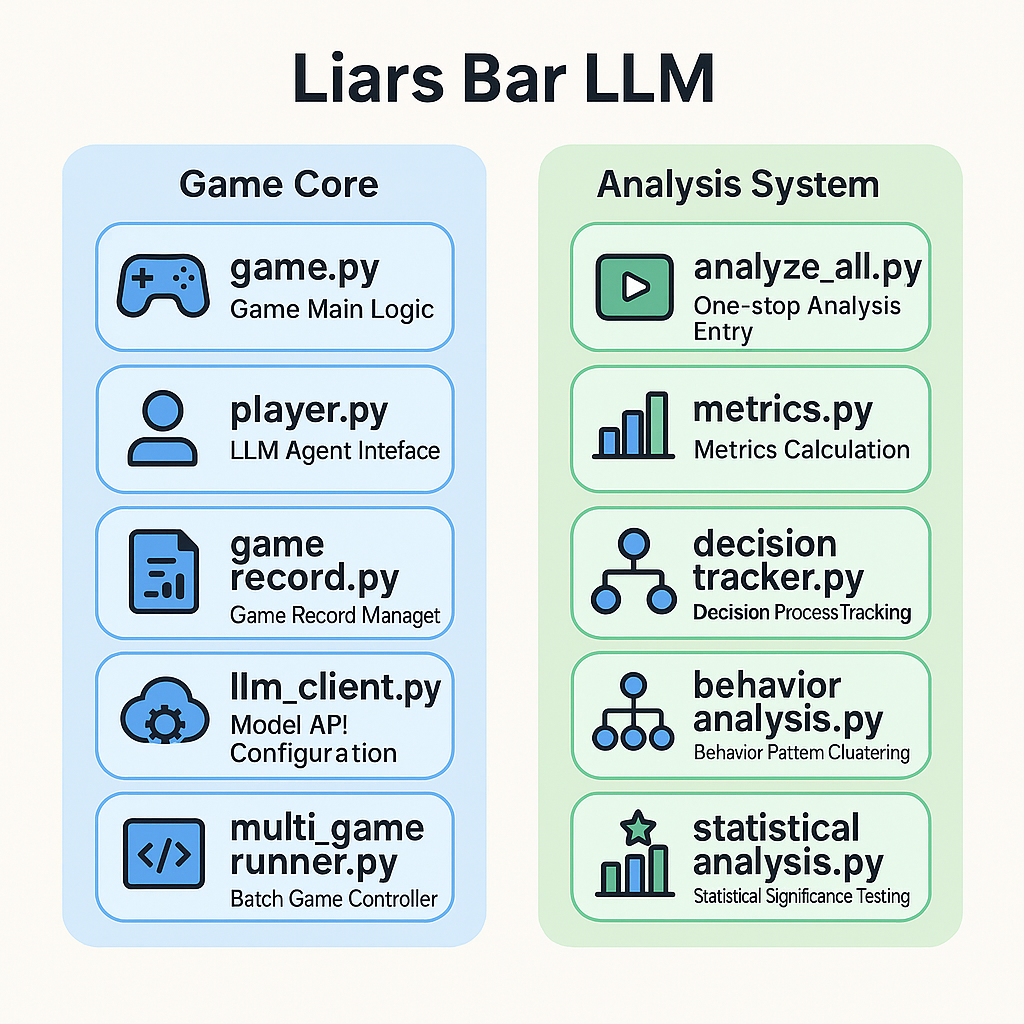
\includegraphics[width=0.9\textwidth]{figures/project_structure.png}
    \caption{System architecture showing the relationship between game core and analysis components}
    \label{fig:system_architecture}
\end{figure}

\subsection{Analysis Framework}
To comprehensively evaluate the strategic capabilities of the LLM agents, we developed a multi-dimensional analysis framework that assesses performance across three primary dimensions.

\subsubsection{Deception Capability Assessment}
We analyze deceptive behavior through metrics including:
\begin{itemize}
    \item \textbf{Honest Play Rate:} Proportion of turns where the agent played cards matching their claims
    \item \textbf{Deception Rate:} Frequency of bluffing (playing non-target cards)
    \item \textbf{Pure/Half Bluff Rate:} Distinguishing between complete bluffs and partial bluffs
    \item \textbf{Deception Success Rate:} Proportion of successful bluffs (not challenged)
    \item \textbf{Challenged Rate:} Frequency of being challenged by other players
    \item \textbf{Joker Usage Rate:} Frequency of using Joker cards strategically
\end{itemize}

\subsubsection{Survival Ability Metrics}
We analyze survival effectiveness through:
\begin{itemize}
    \item \textbf{Survival Rate:} Proportion of games where the agent survived to the end
    \item \textbf{Average Survival Points:} Mean remaining points when eliminated or at game end
    \item \textbf{Average Survival Rank:} Mean placement in the elimination order
    \item \textbf{Early Elimination Rate:} Proportion of games where the agent was first eliminated
    \item \textbf{Round Survival Rate:} Proportion of total game rounds survived
\end{itemize}

\subsubsection{Decision Quality Analysis}
We evaluate decision-making quality through:
\begin{itemize}
    \item \textbf{Challenge Precision:} Proportion of challenges that were correct
    \item \textbf{Challenge Recall:} Proportion of actual bluffs that were challenged
    \item \textbf{Challenge Decision Quality:} Combined measure of precision and recall
    \item \textbf{Card Efficiency:} Effectiveness of card usage relative to game outcomes
\end{itemize}

\subsubsection{Behavioral Pattern Analysis}
Beyond quantitative metrics, we perform:
\begin{itemize}
    \item \textbf{Strategy Clustering:} Identifying distinct strategic profiles using k-means clustering
    \item \textbf{Strategy Evolution:} Tracking how strategies adapt over the course of multiple games
    \item \textbf{Opponent-Specific Strategies:} Analyzing how agents adjust their approach based on opponents
\end{itemize}

Figure \ref{fig:analysis_workflow} presents the complete analysis workflow, showing how game data flows through multiple analytical components to generate comprehensive insights into model performance.

\begin{figure}[H]
    \centering
    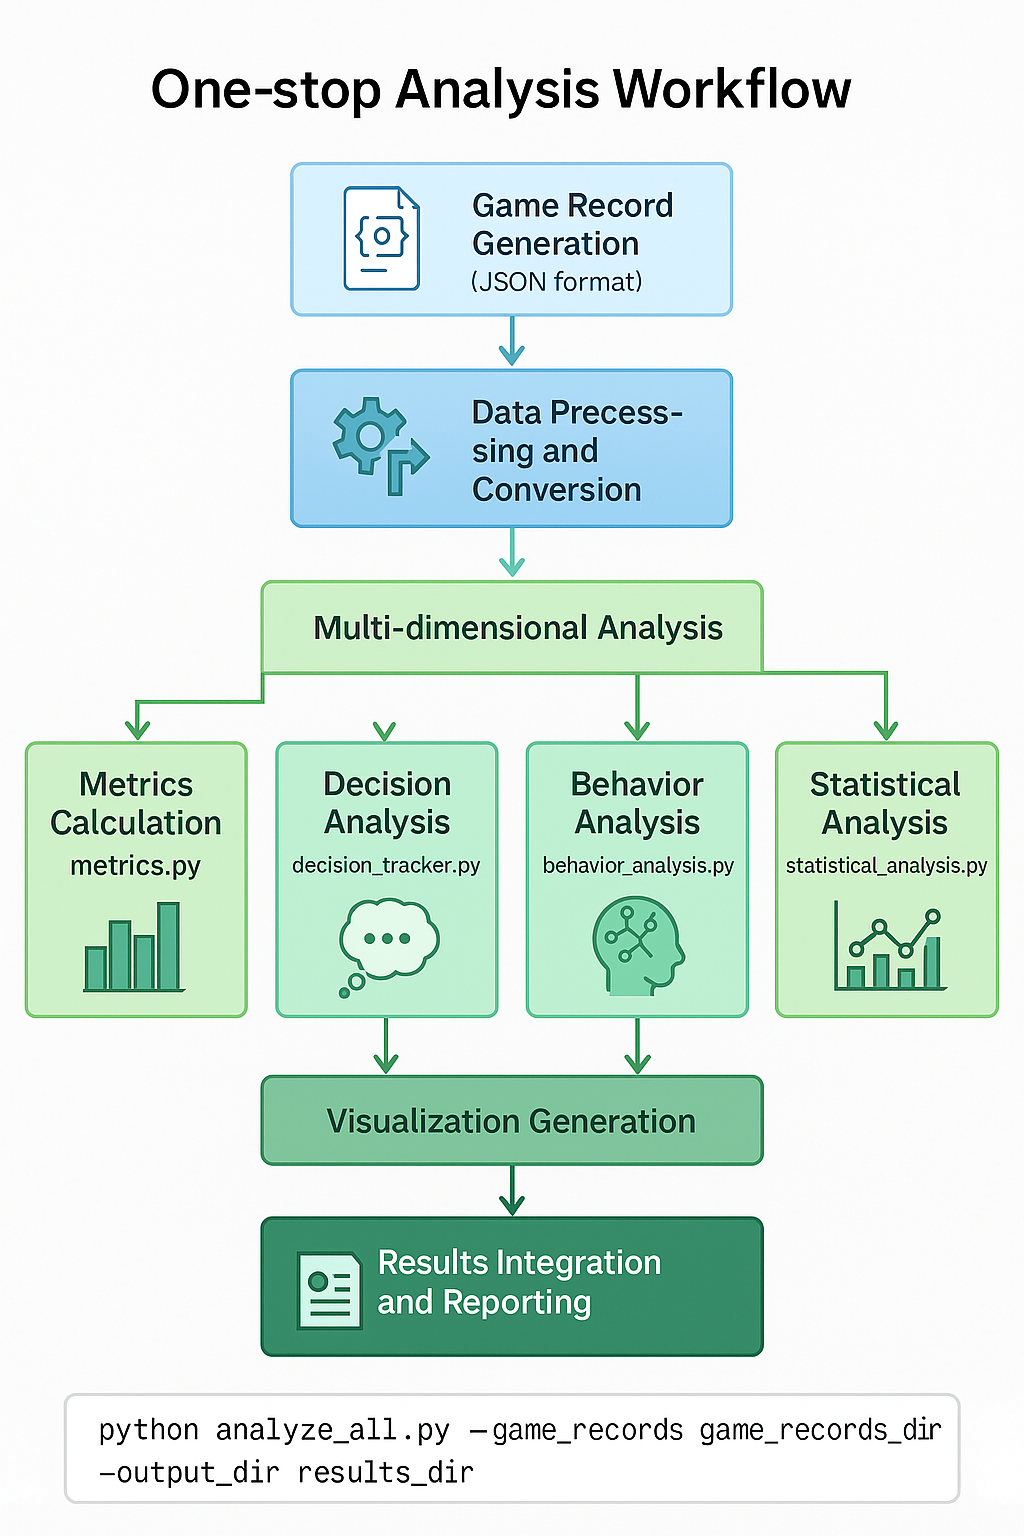
\includegraphics[width=0.9\textwidth]{figures/analysis_flow.png}
    \caption{Analysis workflow showing the processing of game data through multiple analytical components}
    \label{fig:analysis_workflow}
\end{figure}

\subsubsection{Statistical Validation}
To ensure the reliability of our findings, we apply:
\begin{itemize}
    \item \textbf{Parametric Tests:} t-tests, ANOVA, and Tukey HSD post-hoc tests for comparing model performance
    \item \textbf{Non-parametric Tests:} Mann-Whitney U and Kruskal-Wallis H tests for distribution-agnostic comparisons
    \item \textbf{Significance Thresholds:} Standard $\alpha < 0.05$ criterion for statistical significance
\end{itemize}

This comprehensive methodology allows us to systematically evaluate and compare the strategic intelligence and deception capabilities of different LLMs in a controlled, competitive environment.

\section{Results}
Based on our comprehensive analysis of 50 game sessions involving four prominent LLMs, we observed distinct strategic profiles and significant performance differences across models. This section presents our key findings organized around the three primary dimensions of our analysis framework: deception capability, survival ability, and decision quality. The overall performance comparison across all models is visualized in Figure \ref{fig:overall_radar}, which serves as a comprehensive summary of our findings.

\subsection{Deception Capability Analysis}
Our analysis of deceptive behavior revealed clear differences in how each model approached honesty and bluffing strategies.

\subsubsection{Honesty and Bluffing Patterns}
ChatGPT demonstrated the highest honesty rate (92.1\%), showing a strong preference for truthful play. In contrast, Gemini exhibited the lowest honesty rate (68.5\%) and highest overall deception rate (31.5\%), with a particularly high rate of pure bluffing (23.6\%)—playing cards that were entirely different from what was claimed. These contrasting honesty patterns are clearly illustrated in Figure \ref{fig:honest_play_rate}.

\begin{figure}[H]
    \centering
    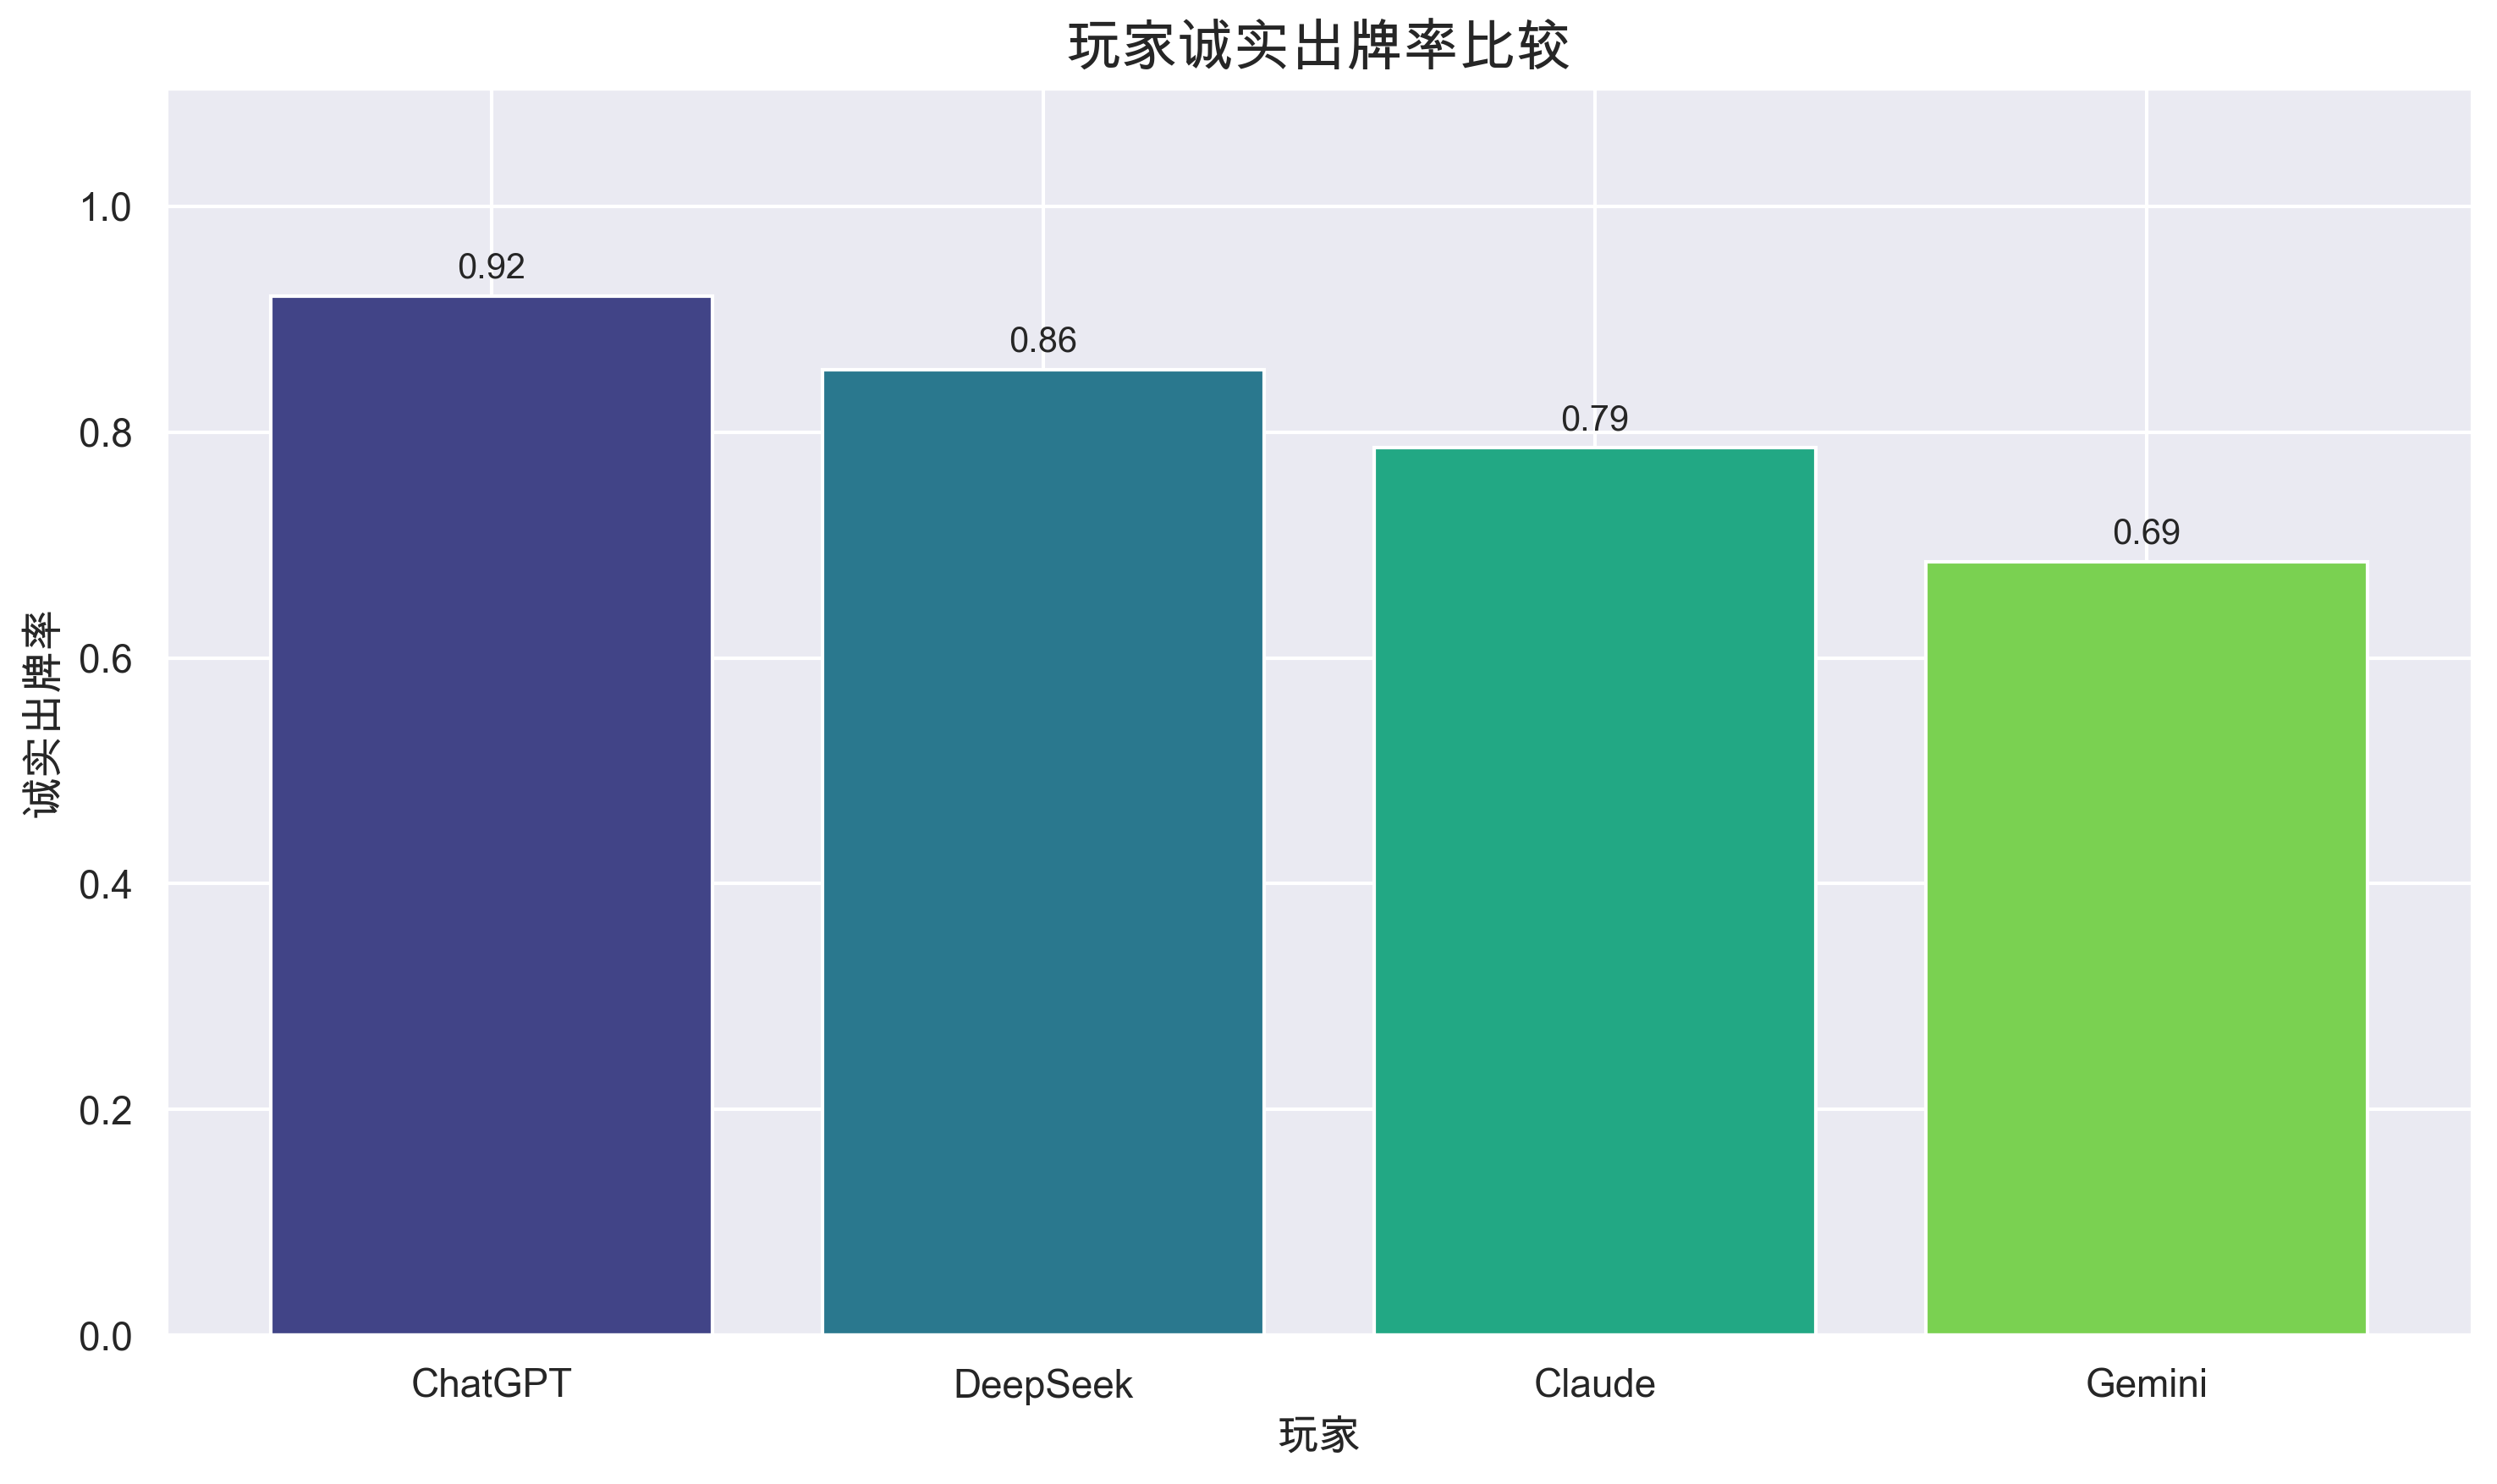
\includegraphics[width=0.9\textwidth]{figures/deception_honest_play_rate.png}
    \caption{Comparison of honest play rates across the four LLM agents}
    \label{fig:honest_play_rate}
\end{figure}

DeepSeek maintained a relatively high honesty rate (85.5\%) while Claude showed moderate honesty (78.6\%). This suggests that different LLMs have inherent tendencies toward truthfulness or deception, even when facing identical game scenarios. The comprehensive comparison of these deception-related metrics can be seen in Figure \ref{fig:deception_radar}, which visualizes the different strategic profiles of each model.

\begin{figure}[H]
    \centering
    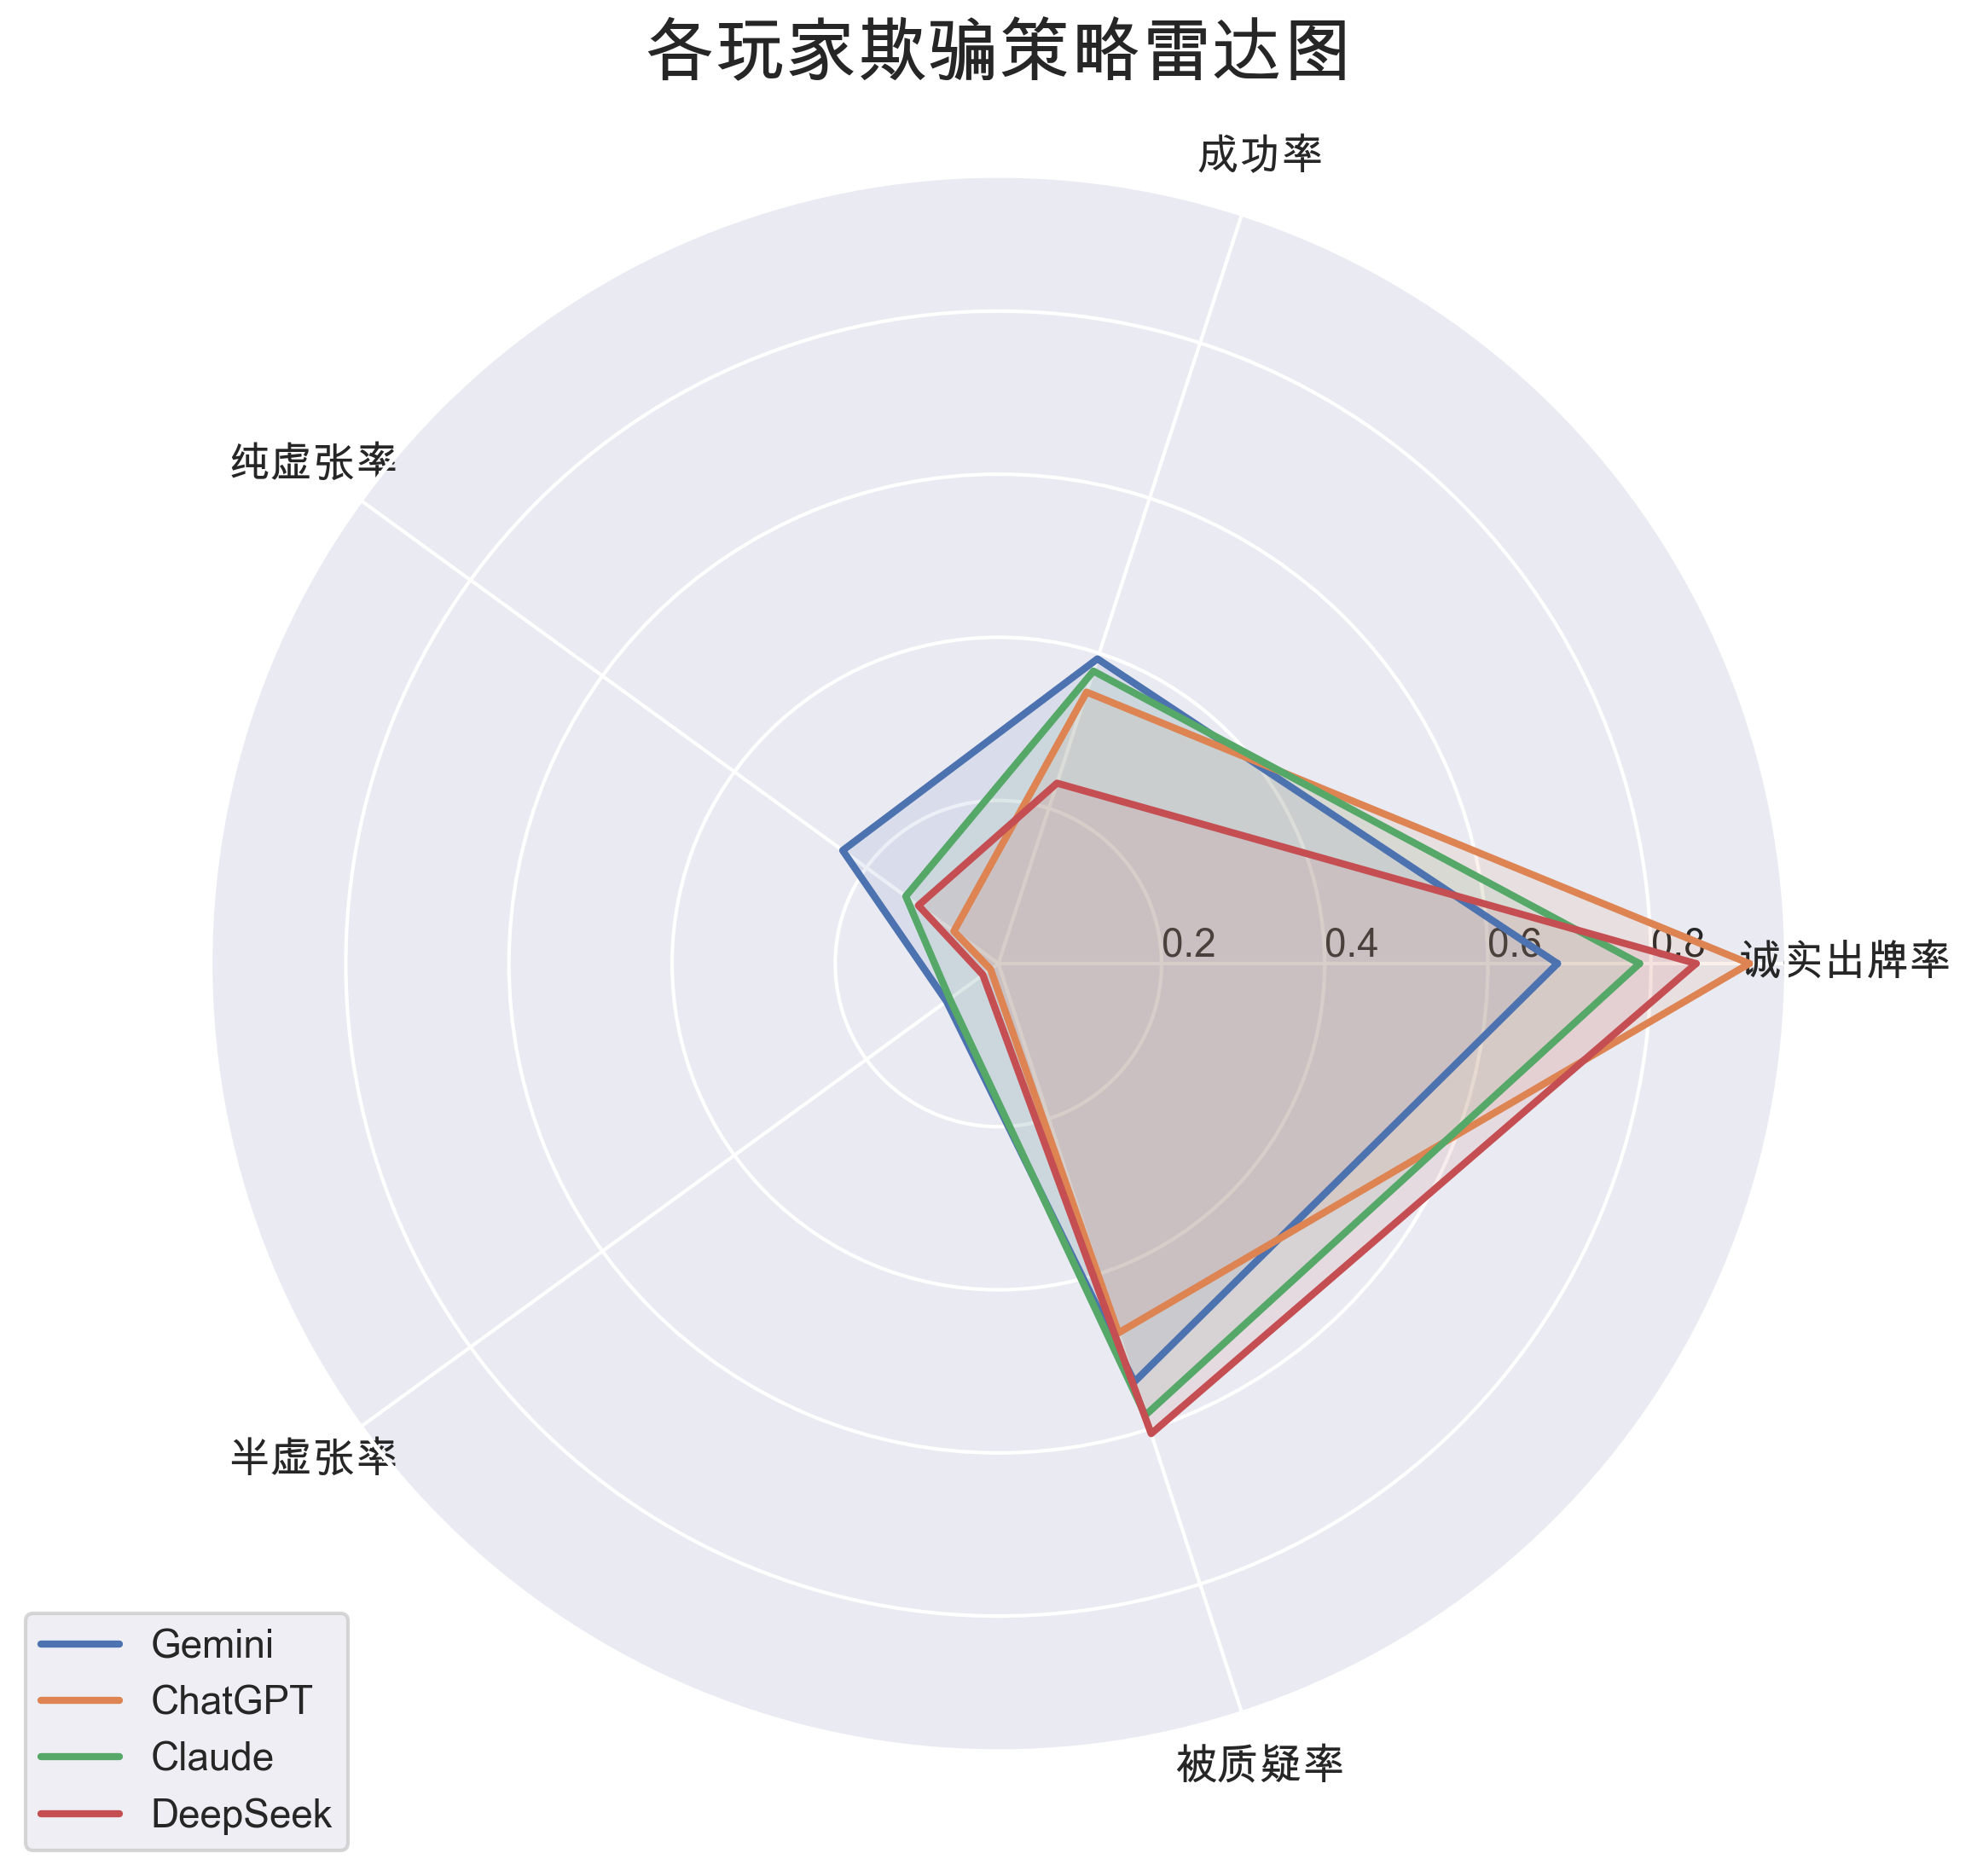
\includegraphics[width=0.9\textwidth]{figures/deception_radar.png}
    \caption{Radar chart comparing deception-related metrics across models}
    \label{fig:deception_radar}
\end{figure}

\subsubsection{Bluffing Strategy Analysis}
We observed distinct bluffing patterns among the models:
\begin{itemize}
    \item \textbf{Pure vs. Half Bluffs:} Gemini and Claude showed higher propensity for half-bluffing (mixing target and non-target cards) compared to ChatGPT, suggesting more sophisticated deception strategies.
    \item \textbf{Joker Usage:} DeepSeek (36.0\%) and ChatGPT (30.6\%) utilized Joker cards most effectively as strategic wild cards, while Claude showed the lowest Joker usage (16.8\%).
    \item \textbf{Deception Success Rate:} Despite bluffing less frequently, Claude achieved the highest deception success rate (37.7\%), indicating more effective timing and execution of bluffs, as shown in Figure \ref{fig:deception_success}.
\end{itemize}

\begin{figure}[H]
    \centering
    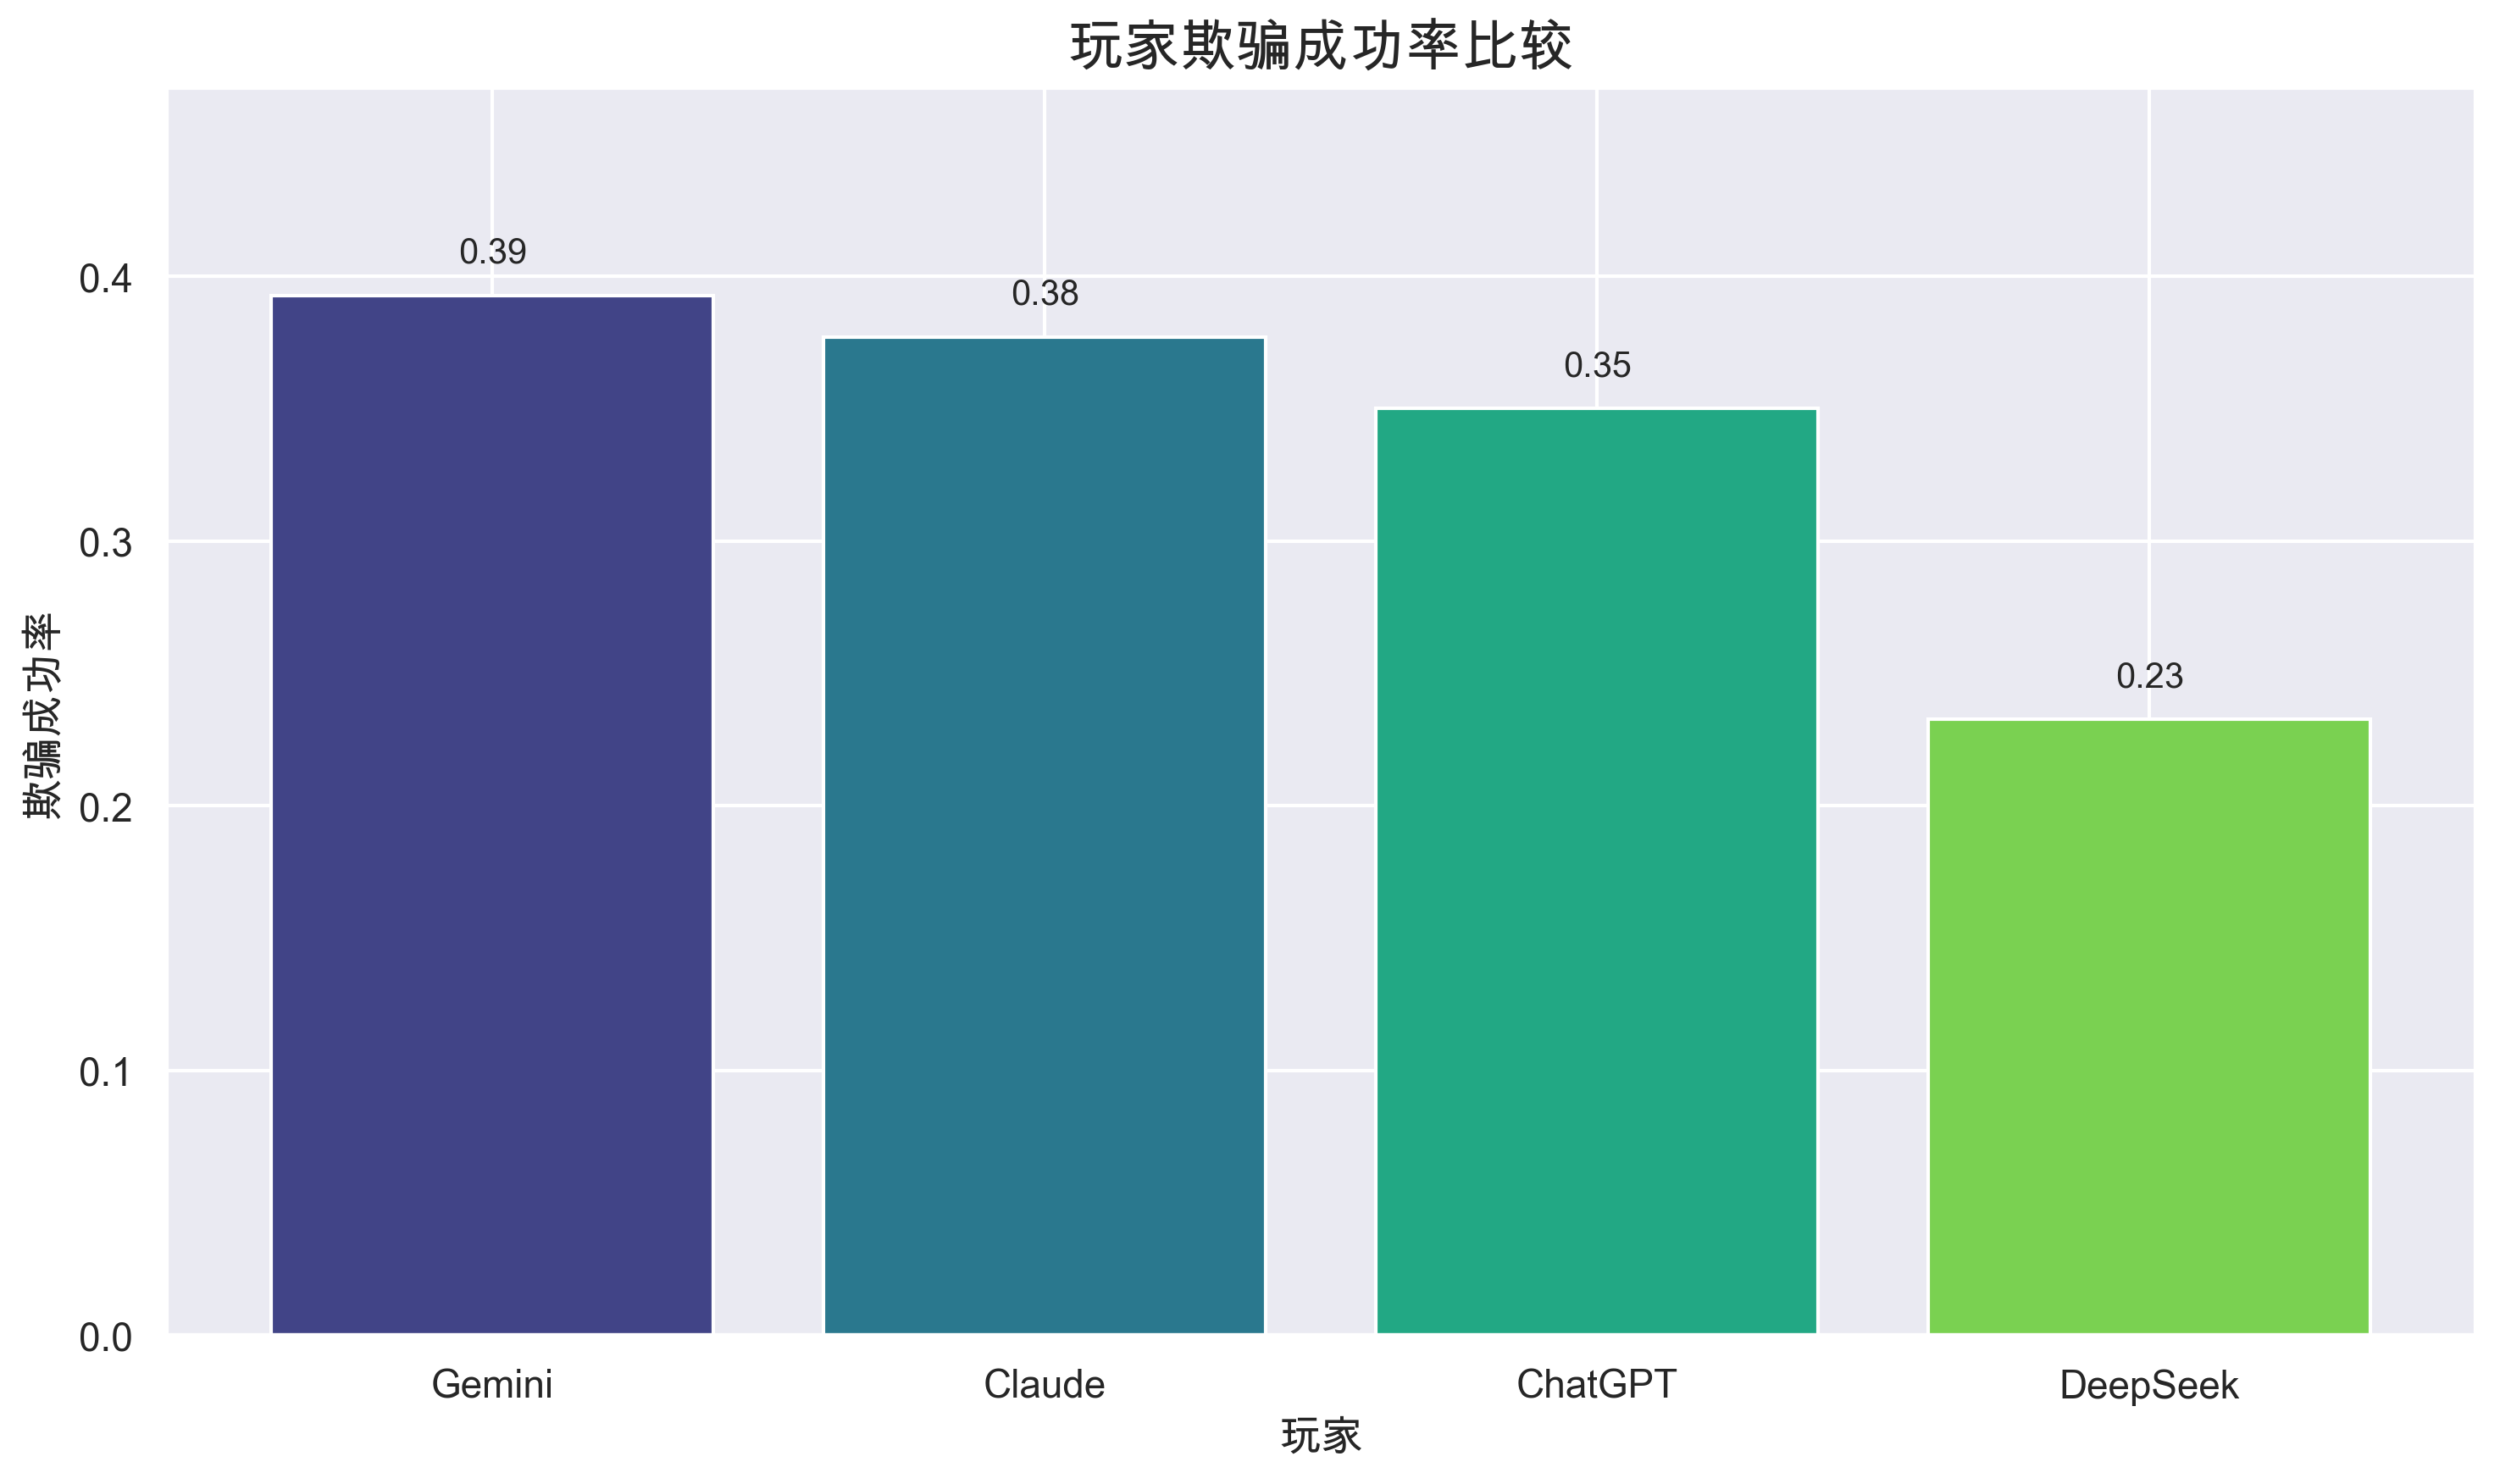
\includegraphics[width=0.9\textwidth]{figures/deception_deception_success_rate.png}
    \caption{Deception success rates showing the proportion of bluffs that were not challenged}
    \label{fig:deception_success}
\end{figure}

Statistical analysis confirmed that the differences in deception patterns were significant ($\alpha < 0.05$), with Gemini's aggressive bluffing strategy and ChatGPT's honest approach representing opposite ends of the spectrum.

\subsection{Survival Ability Analysis}
The second dimension of our analysis examined how effectively each model survived in the competitive environment.

\subsubsection{Win Rate and Survival Metrics}
DeepSeek demonstrated superior survival ability, winning 44\% of games—significantly higher than other models. This was correlated with maintaining the highest average survival points (51.2) across all games, as depicted in Figure \ref{fig:survival_points}.

\begin{figure}[H]
    \centering
    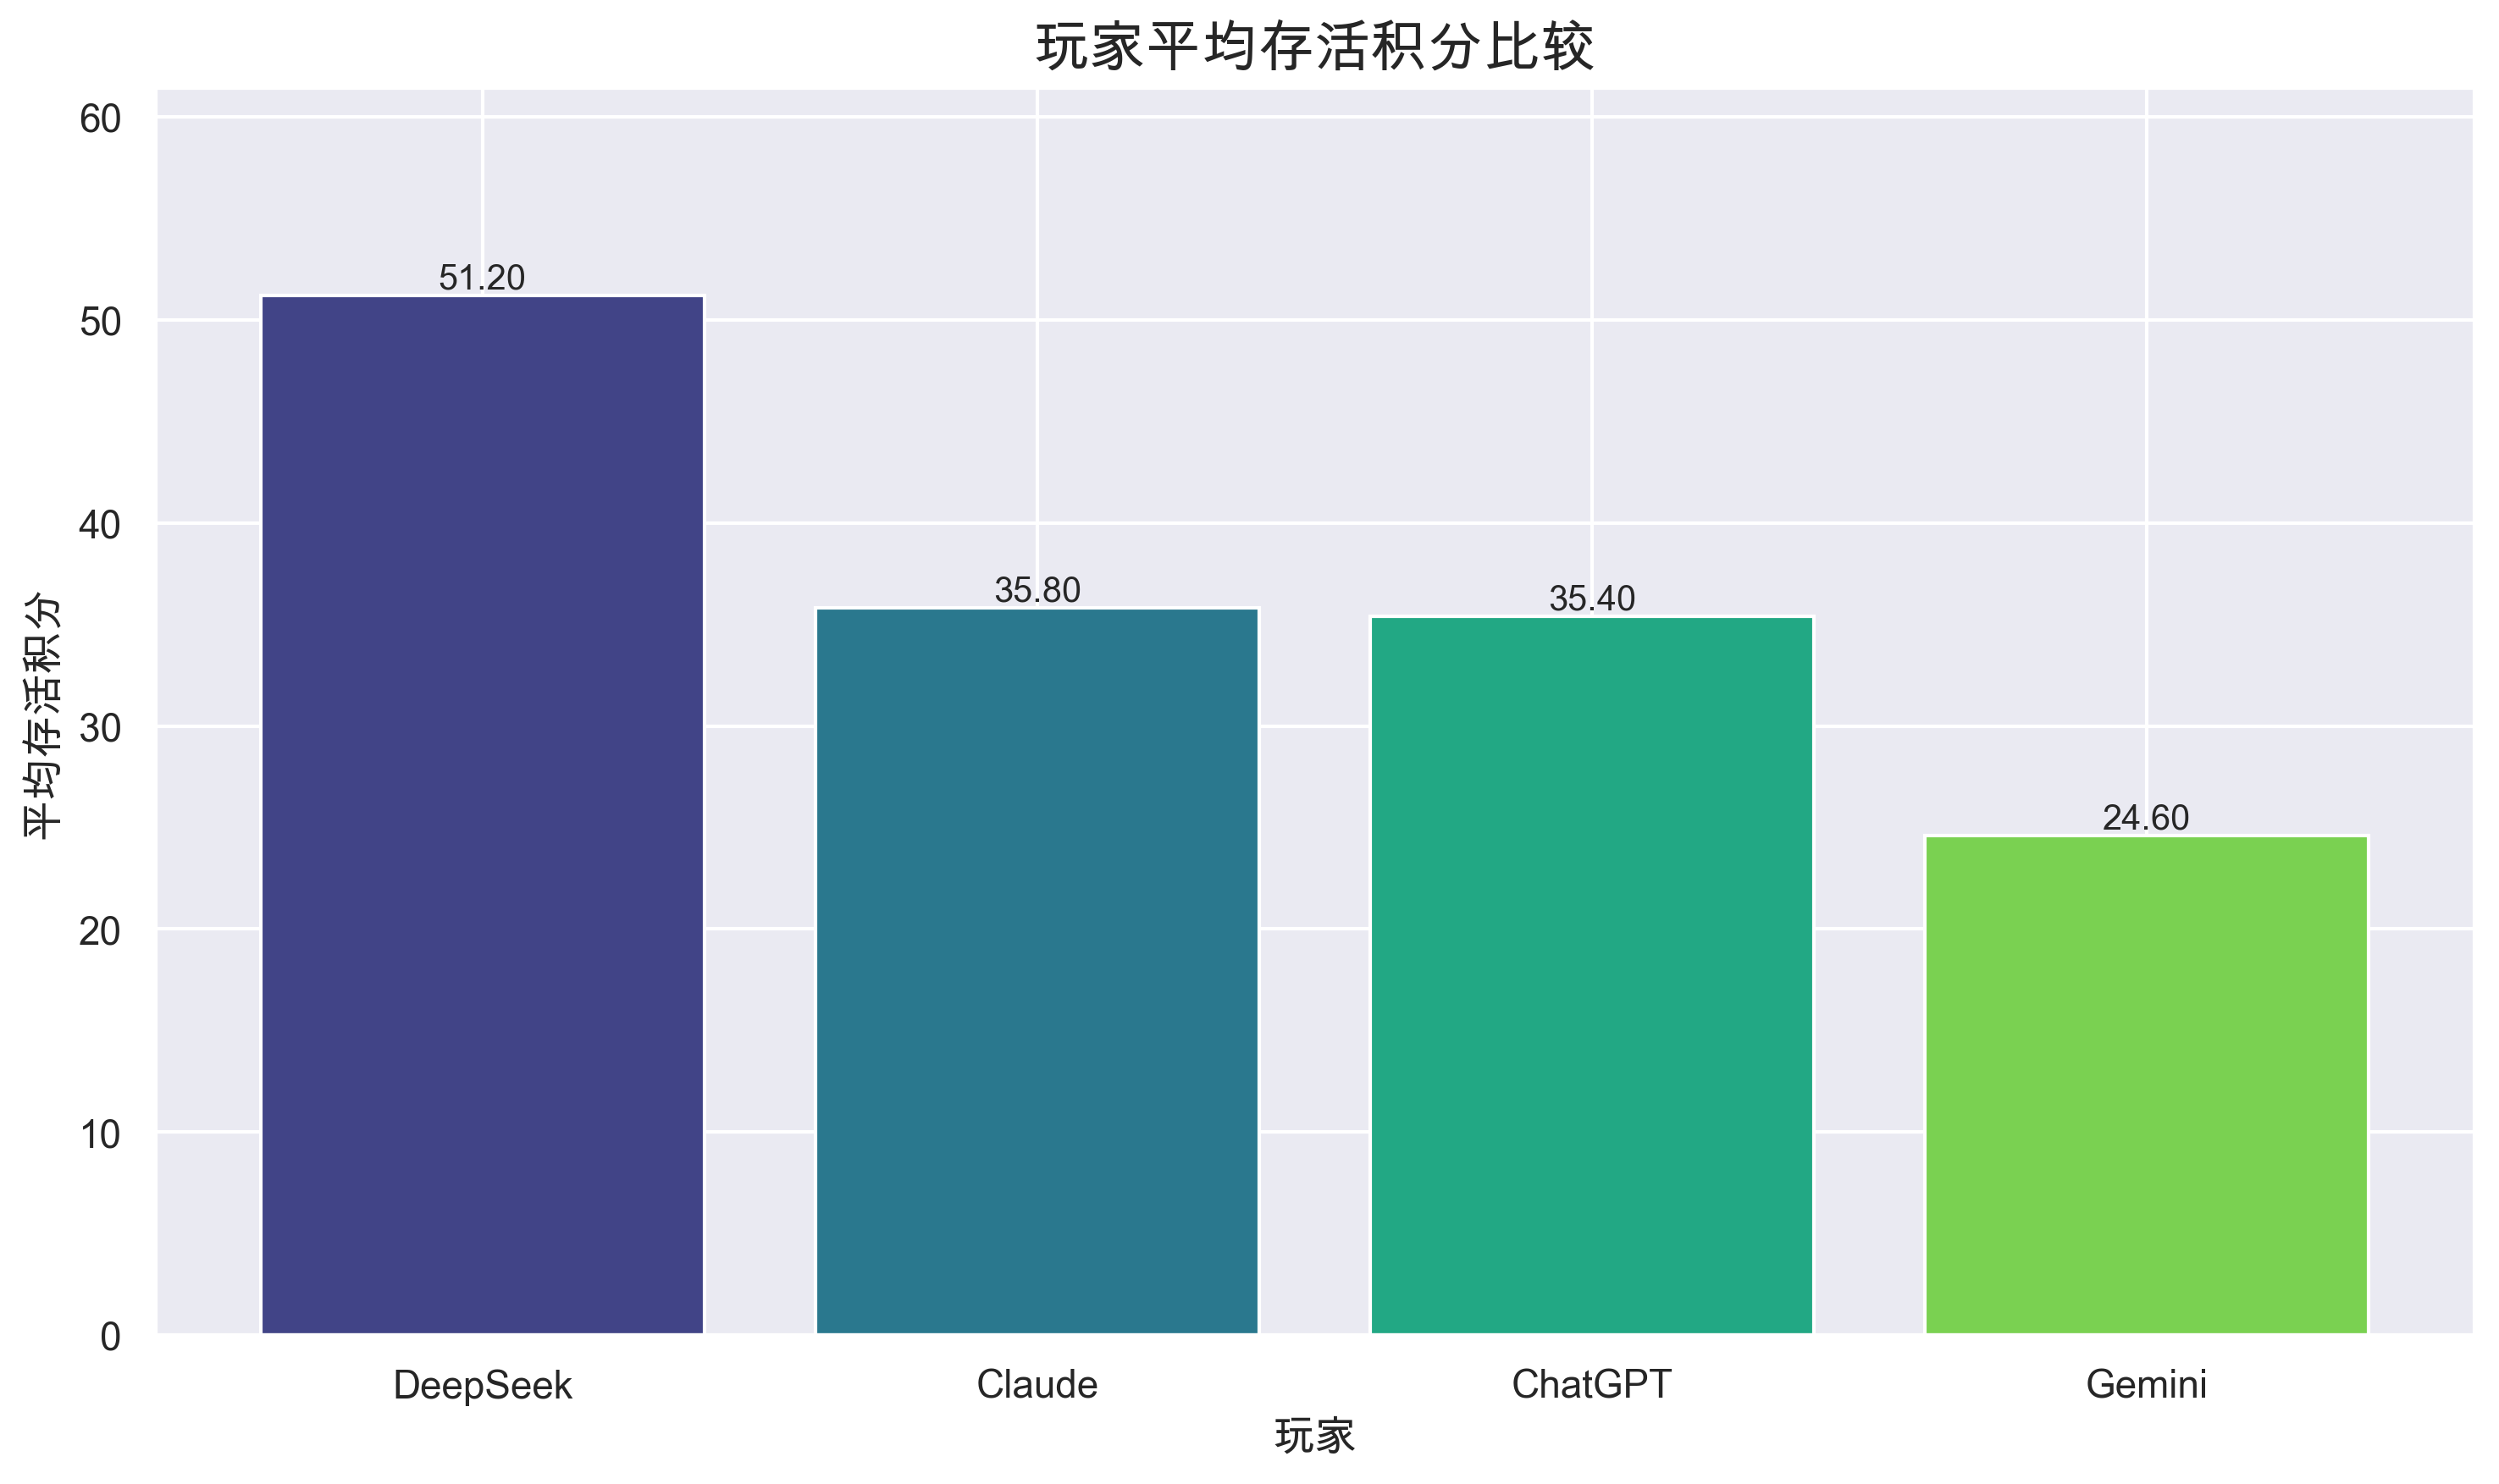
\includegraphics[width=0.9\textwidth]{figures/survival_average_survival_points.png}
    \caption{Average survival points for each LLM agent across all games}
    \label{fig:survival_points}
\end{figure}

Claude and ChatGPT showed moderate performance (26\% and 22\% win rates respectively), while Gemini's aggressive strategy resulted in the lowest win rate (8\%) and average survival points (24.6). The detailed elimination patterns and win distributions across different matchups are visualized in Figure \ref{fig:survival_matrix}.

\begin{figure}[H]
    \centering
    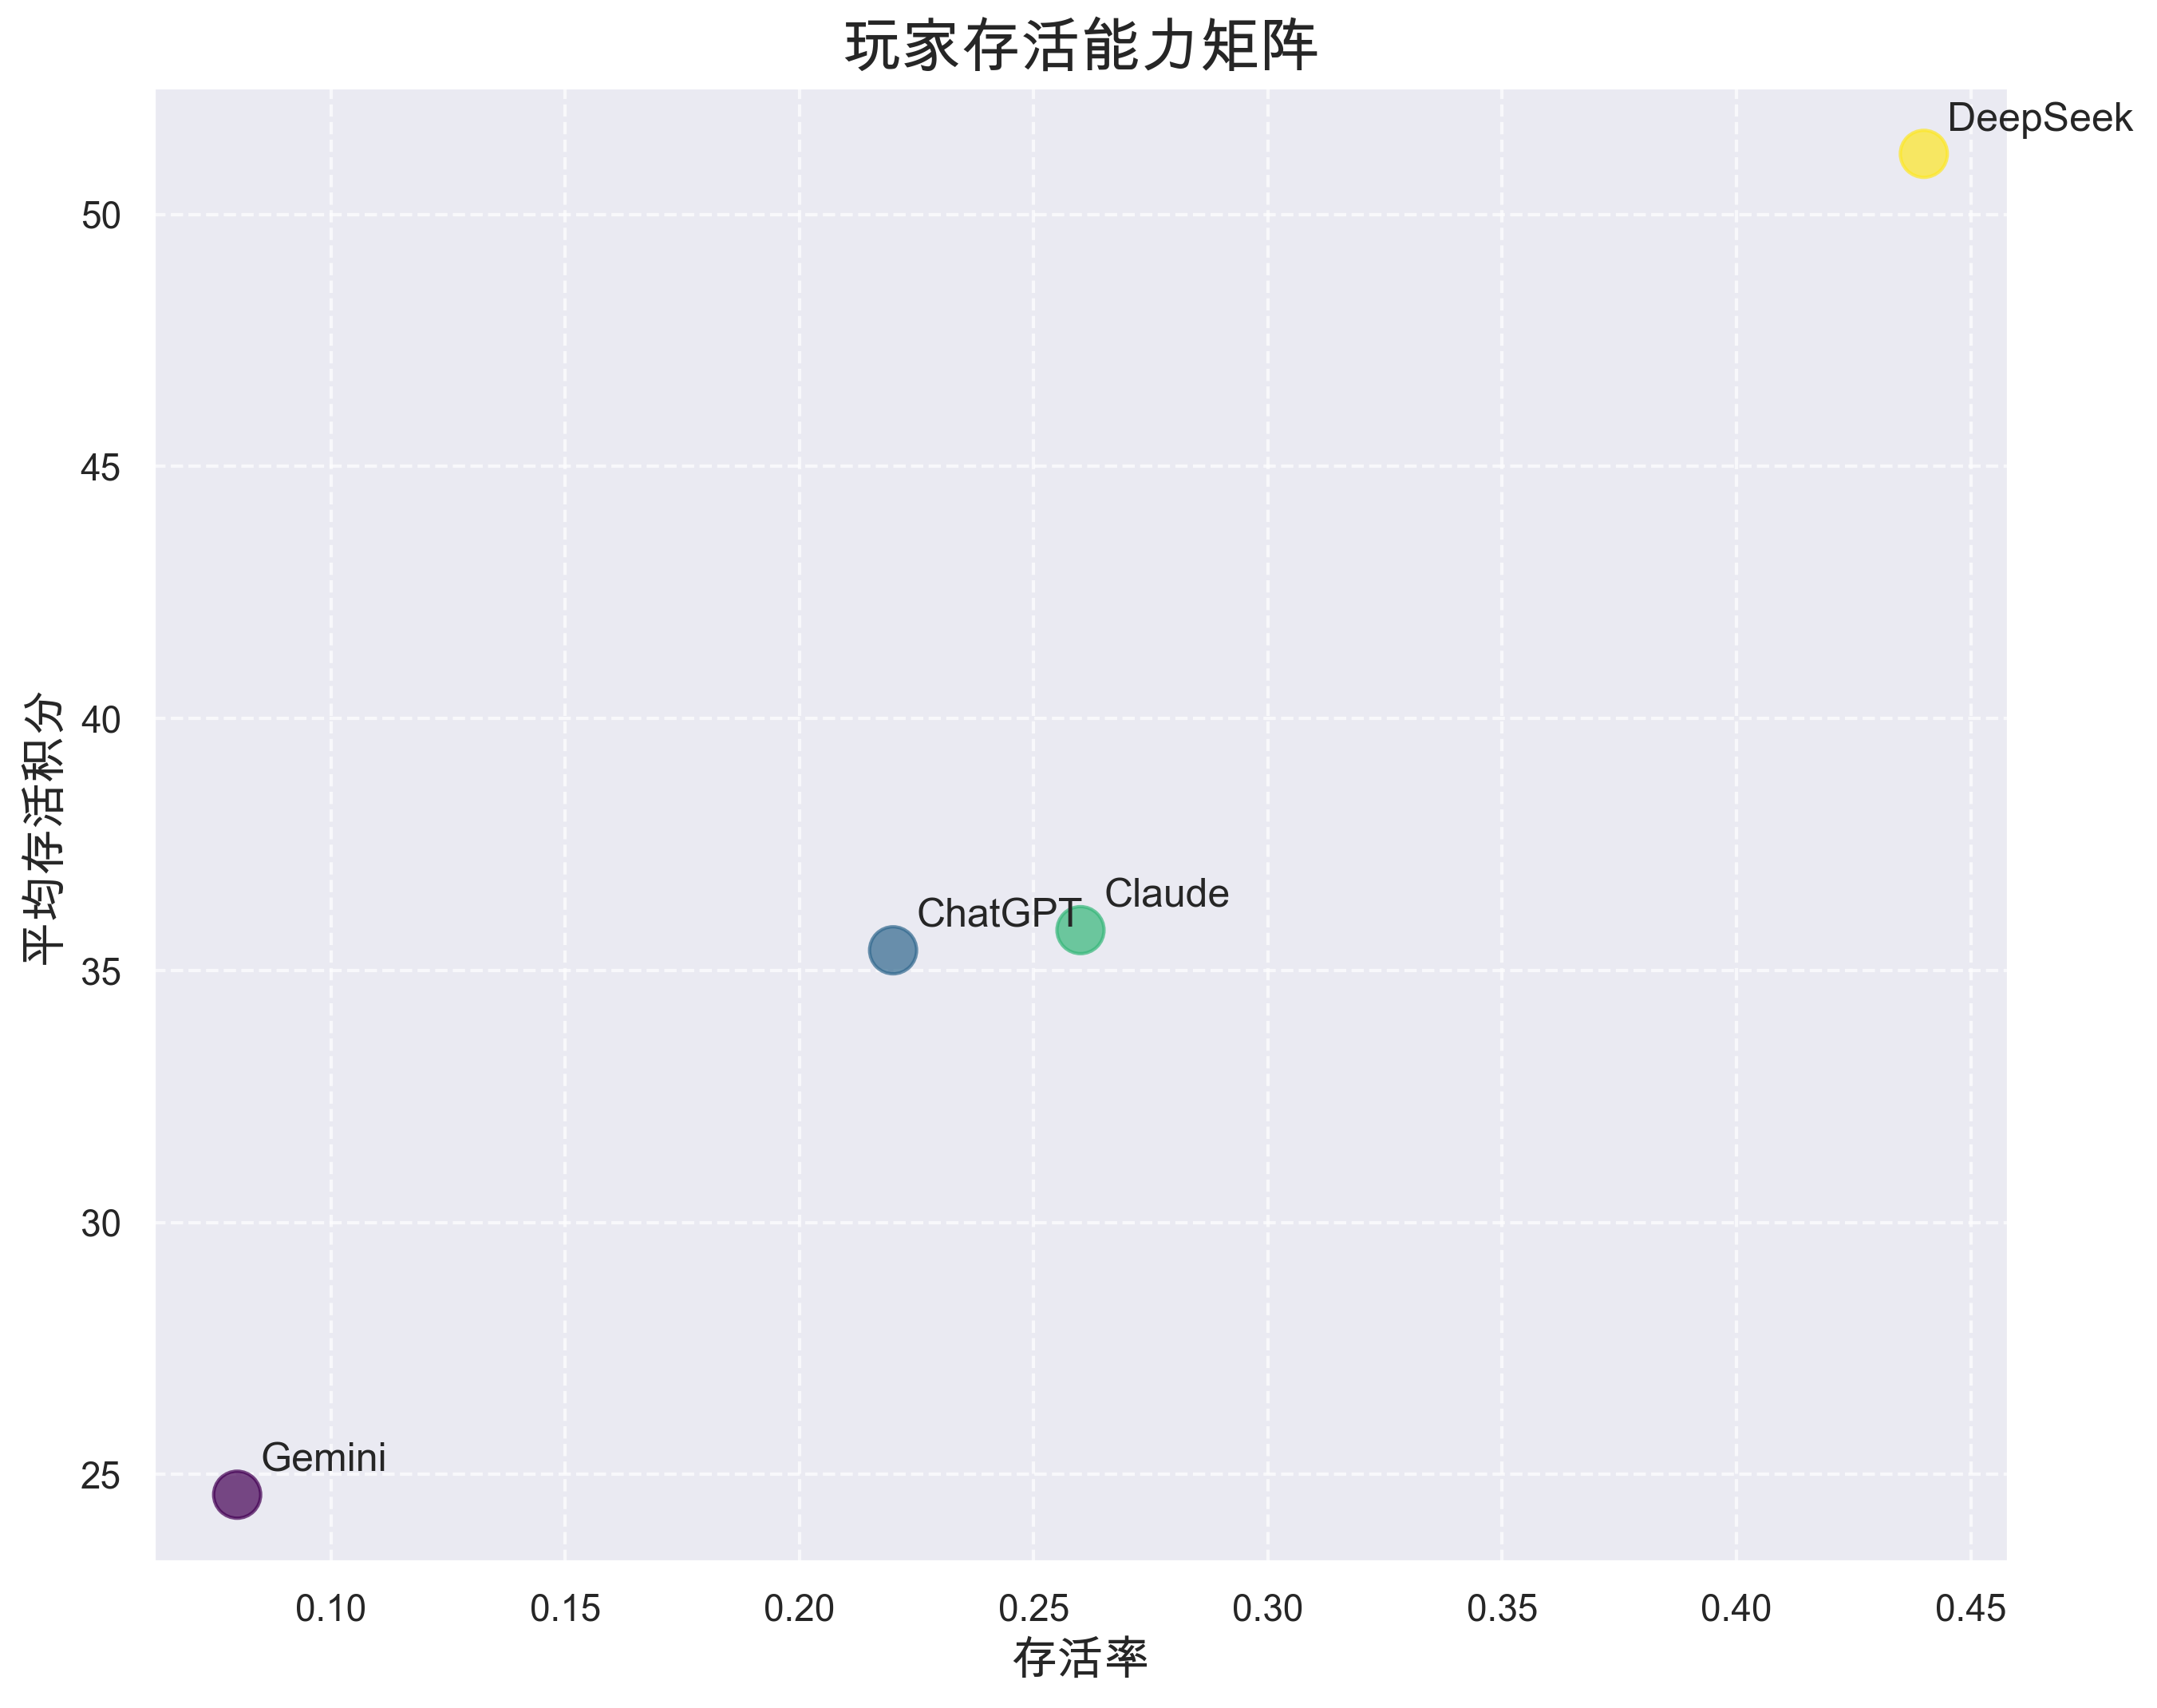
\includegraphics[width=0.9\textwidth]{figures/survival_matrix.png}
    \caption{Survival matrix showing elimination patterns and win distributions}
    \label{fig:survival_matrix}
\end{figure}

\subsubsection{Elimination Patterns}
Analysis of elimination patterns revealed:
\begin{itemize}
    \item \textbf{Early Elimination:} ChatGPT faced the highest early elimination rate (30\%), despite its conservative play style. This suggests that excessive honesty may be detrimental in competitive environments requiring strategic deception.
    \item \textbf{Round Survival:} DeepSeek (78.9\%) and Claude (77.9\%) demonstrated the highest round survival rates, indicating more effective long-term strategy management.
    \item \textbf{Survival Ranking:} The average survival rank showed DeepSeek (2.92) consistently outlasting other models, with Gemini (2.06) most frequently being eliminated early.
\end{itemize}

Figure \ref{fig:early_elimination} illustrates the early elimination rates, highlighting the vulnerability of certain strategic approaches in the game's competitive environment.

\begin{figure}[H]
    \centering
    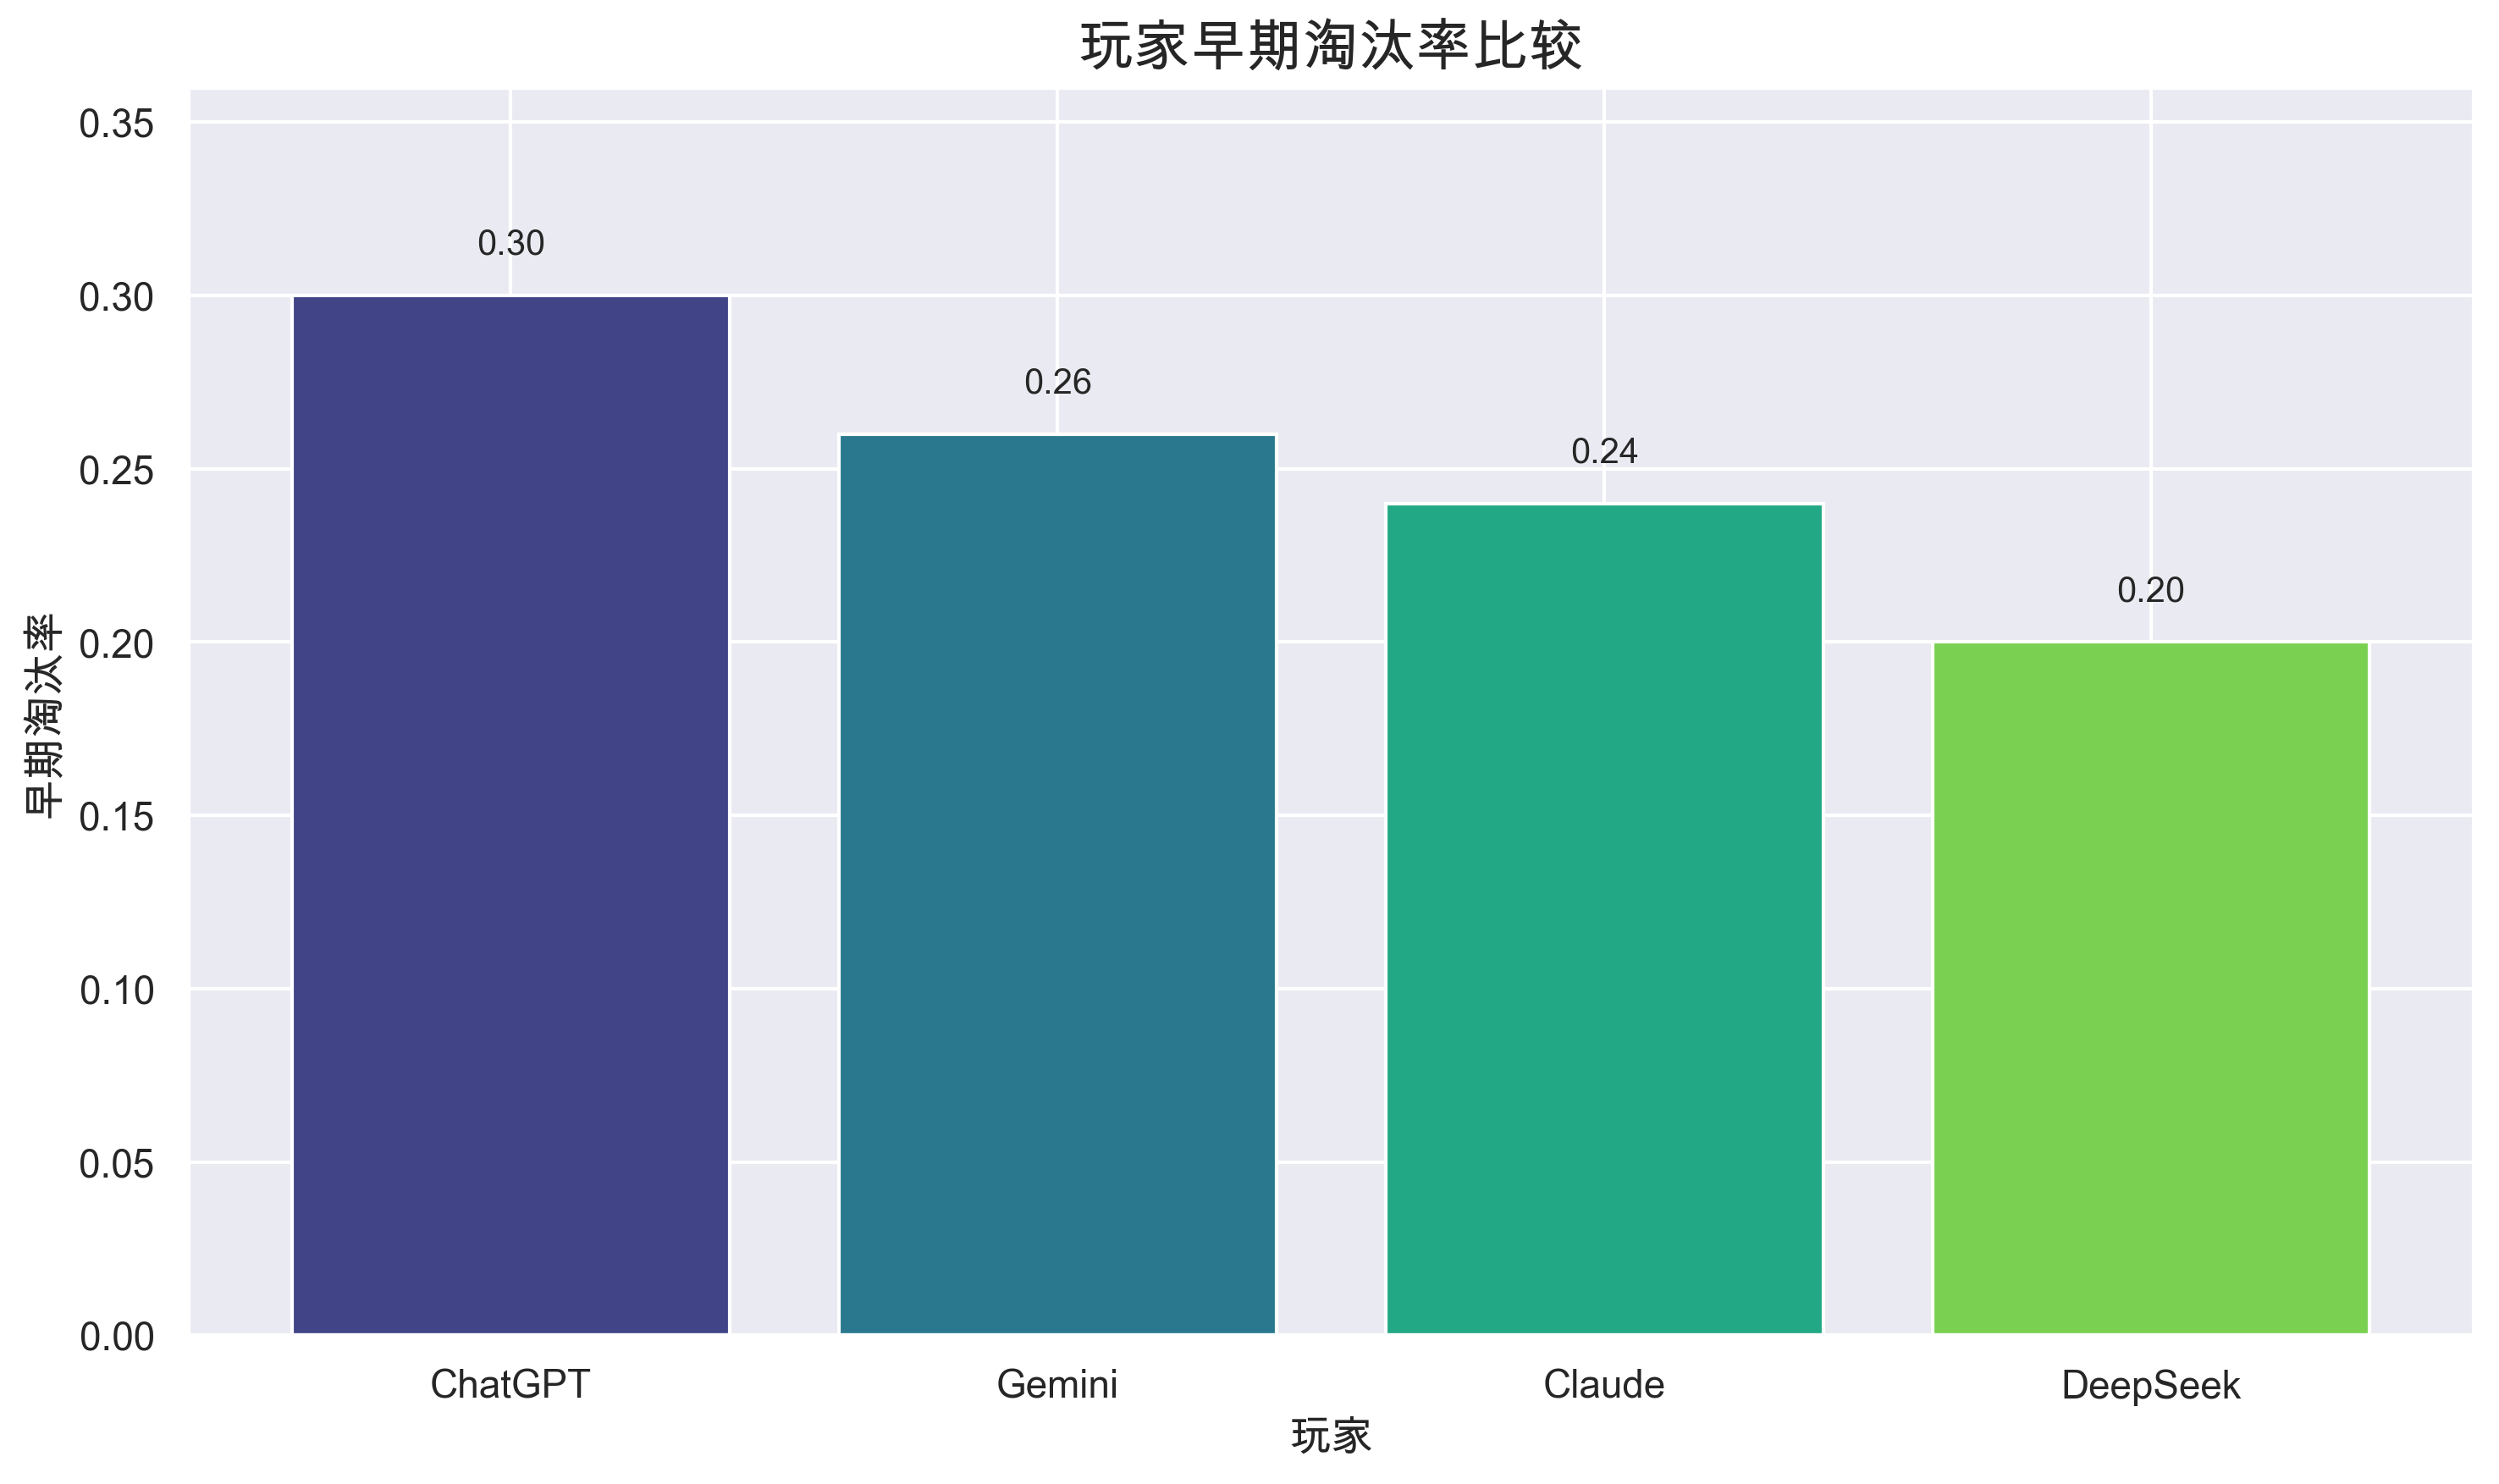
\includegraphics[width=0.9\textwidth]{figures/survival_early_elimination_rate.png}
    \caption{Early elimination rates showing the proportion of games where each model was eliminated first}
    \label{fig:early_elimination}
\end{figure}

The survival metrics highlight that balanced strategic approaches (as demonstrated by DeepSeek) tend to outperform both extremely honest (ChatGPT) and highly deceptive (Gemini) strategies in multi-agent competitive settings.

\subsection{Decision Quality Analysis}
The third dimension focused on evaluating the quality of strategic decisions made by each model.

\subsubsection{Challenge Decision Quality}
When deciding whether to challenge other players' claims:
\begin{itemize}
    \item \textbf{Challenge Precision:} DeepSeek showed the highest precision (22.6\%), successfully identifying actual bluffs when challenging, followed by Gemini (19.0\%).
    \item \textbf{Challenge Recall:} All models demonstrated perfect recall (1.0) for observed bluffs, indicating they consistently recognized and challenged obvious deceptions.
    \item \textbf{Overall Decision Quality:} DeepSeek achieved the highest combined challenge decision quality score (0.37), balancing when to challenge and when to accept claims.
\end{itemize}

The challenge decision quality metrics are visualized in Figure \ref{fig:challenge_quality}, while Figure \ref{fig:decision_quality_comparison} provides a comprehensive comparison of multiple decision quality indicators across all models.

\begin{figure}[H]
    \centering
    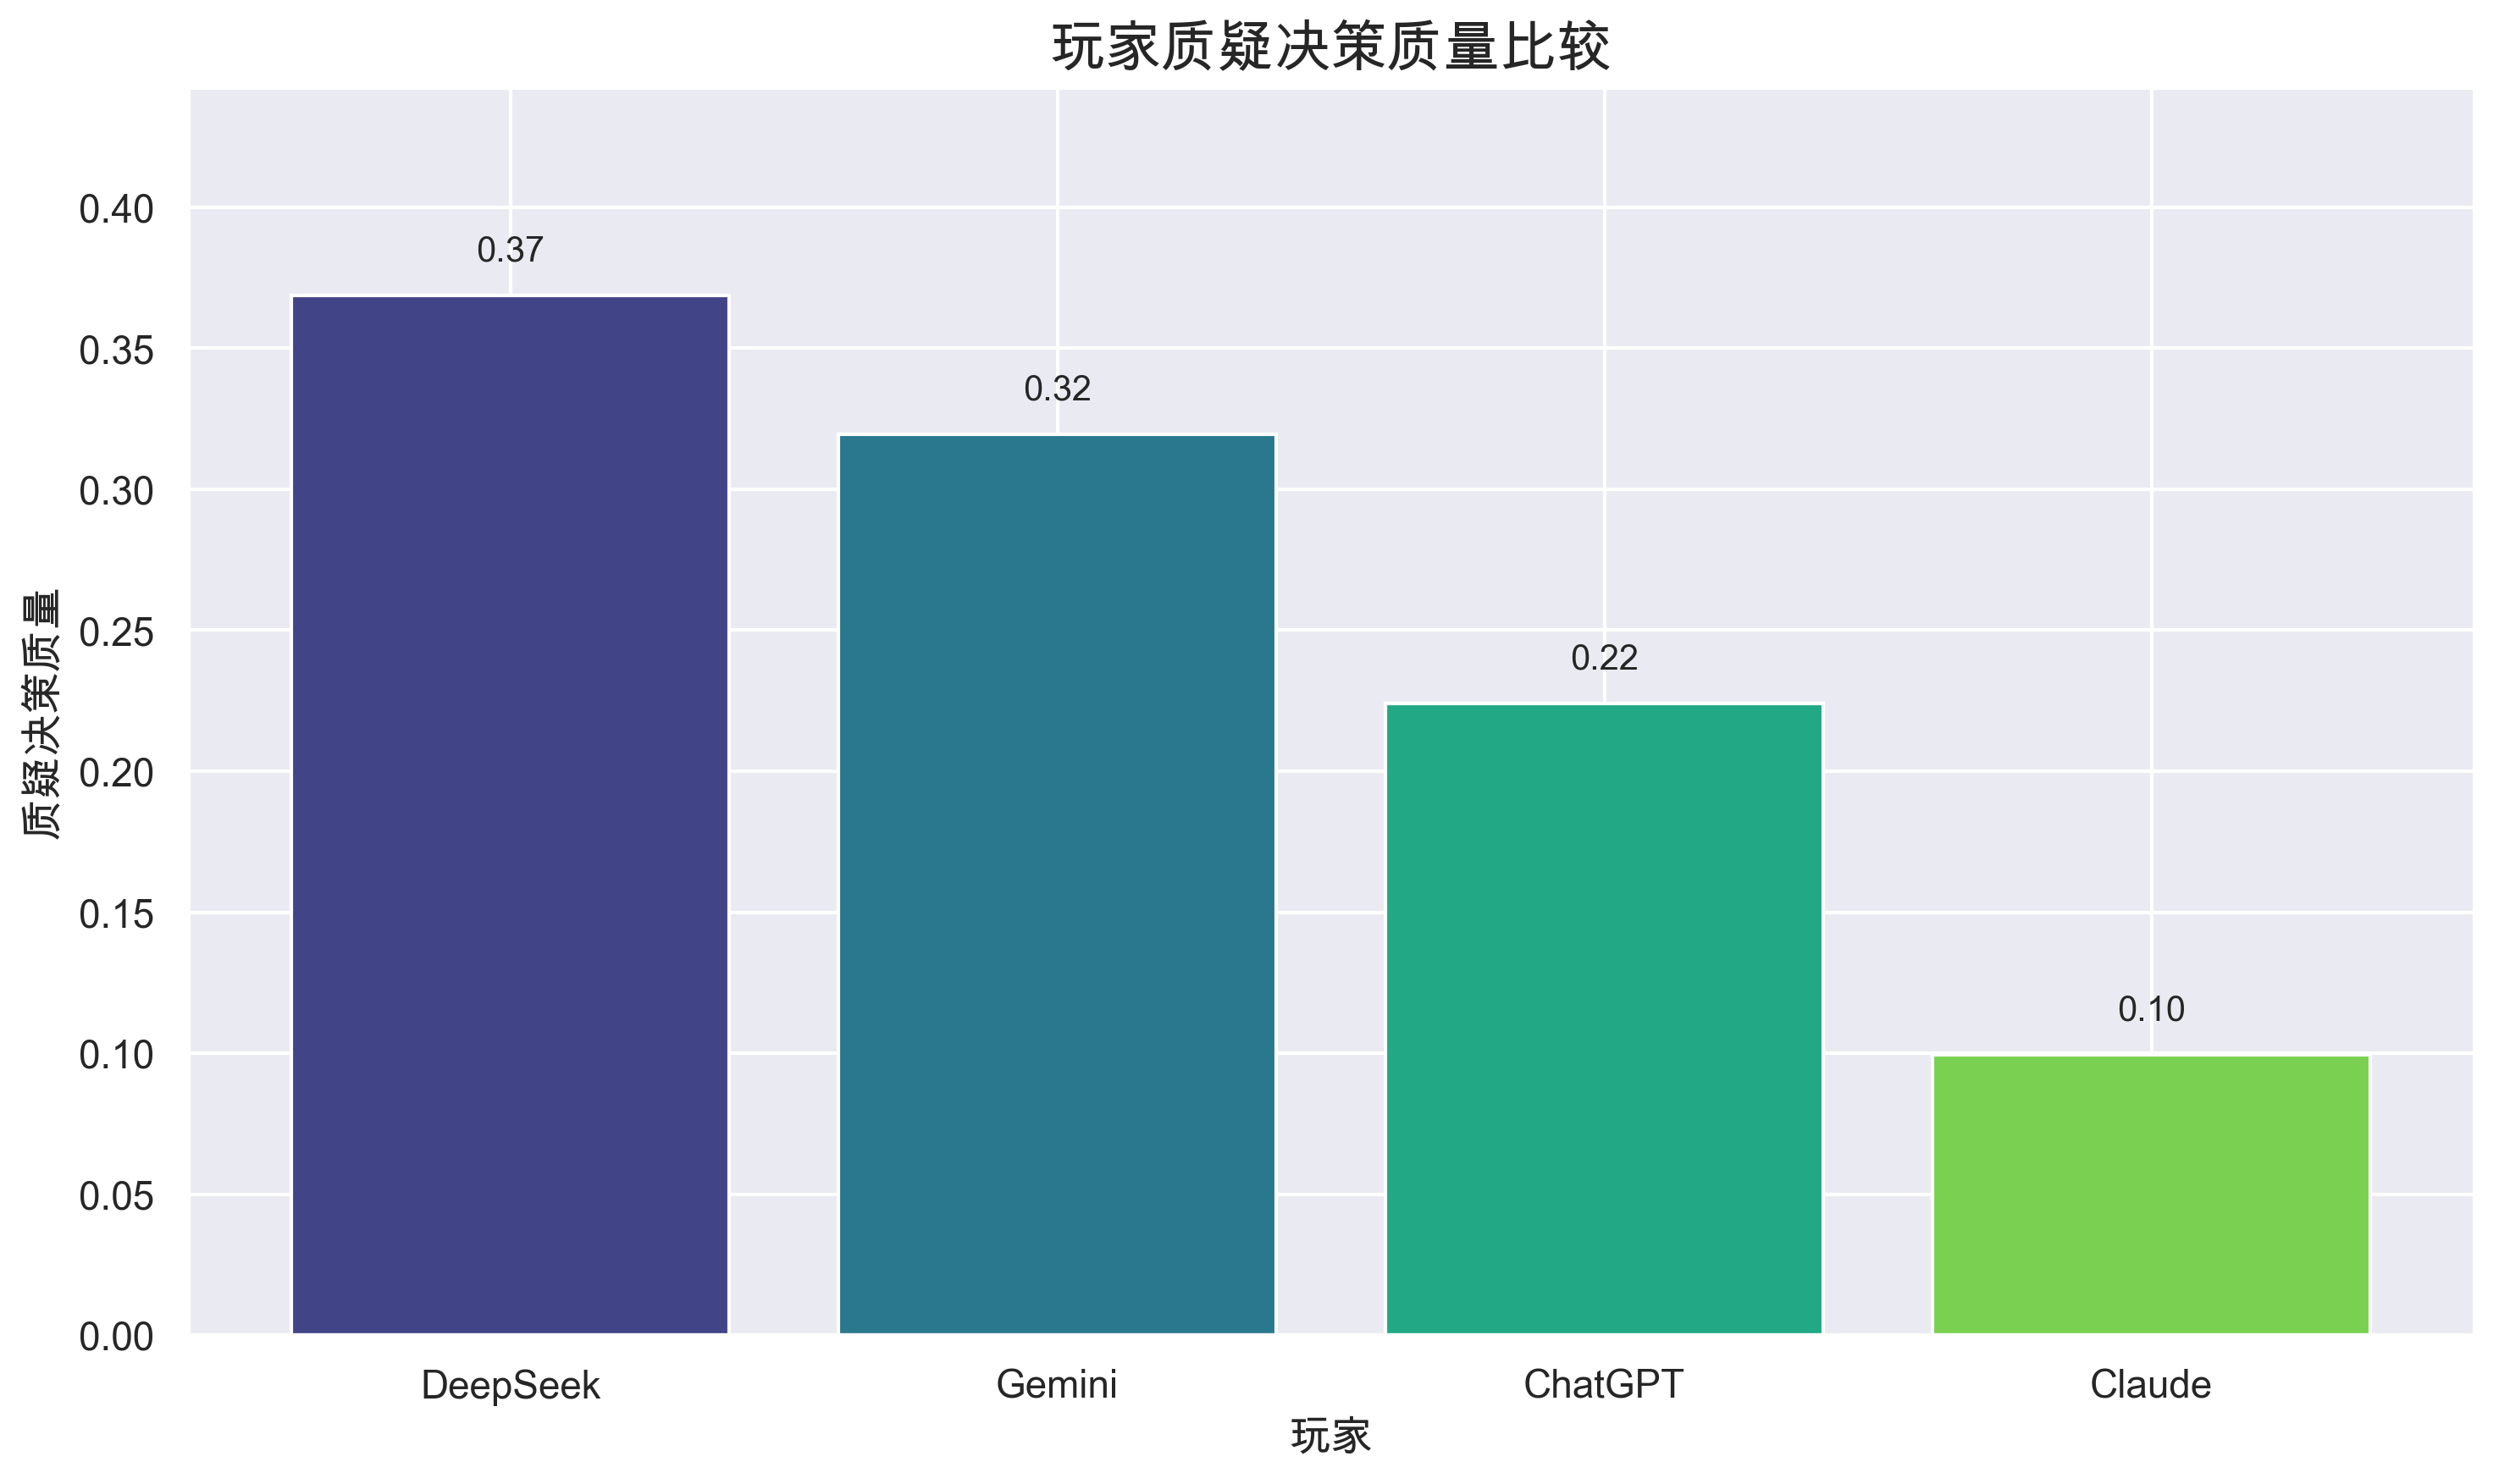
\includegraphics[width=0.9\textwidth]{figures/decision_challenge_decision_quality.png}
    \caption{Challenge decision quality combining precision and recall metrics}
    \label{fig:challenge_quality}
\end{figure}

\begin{figure}[H]
    \centering
    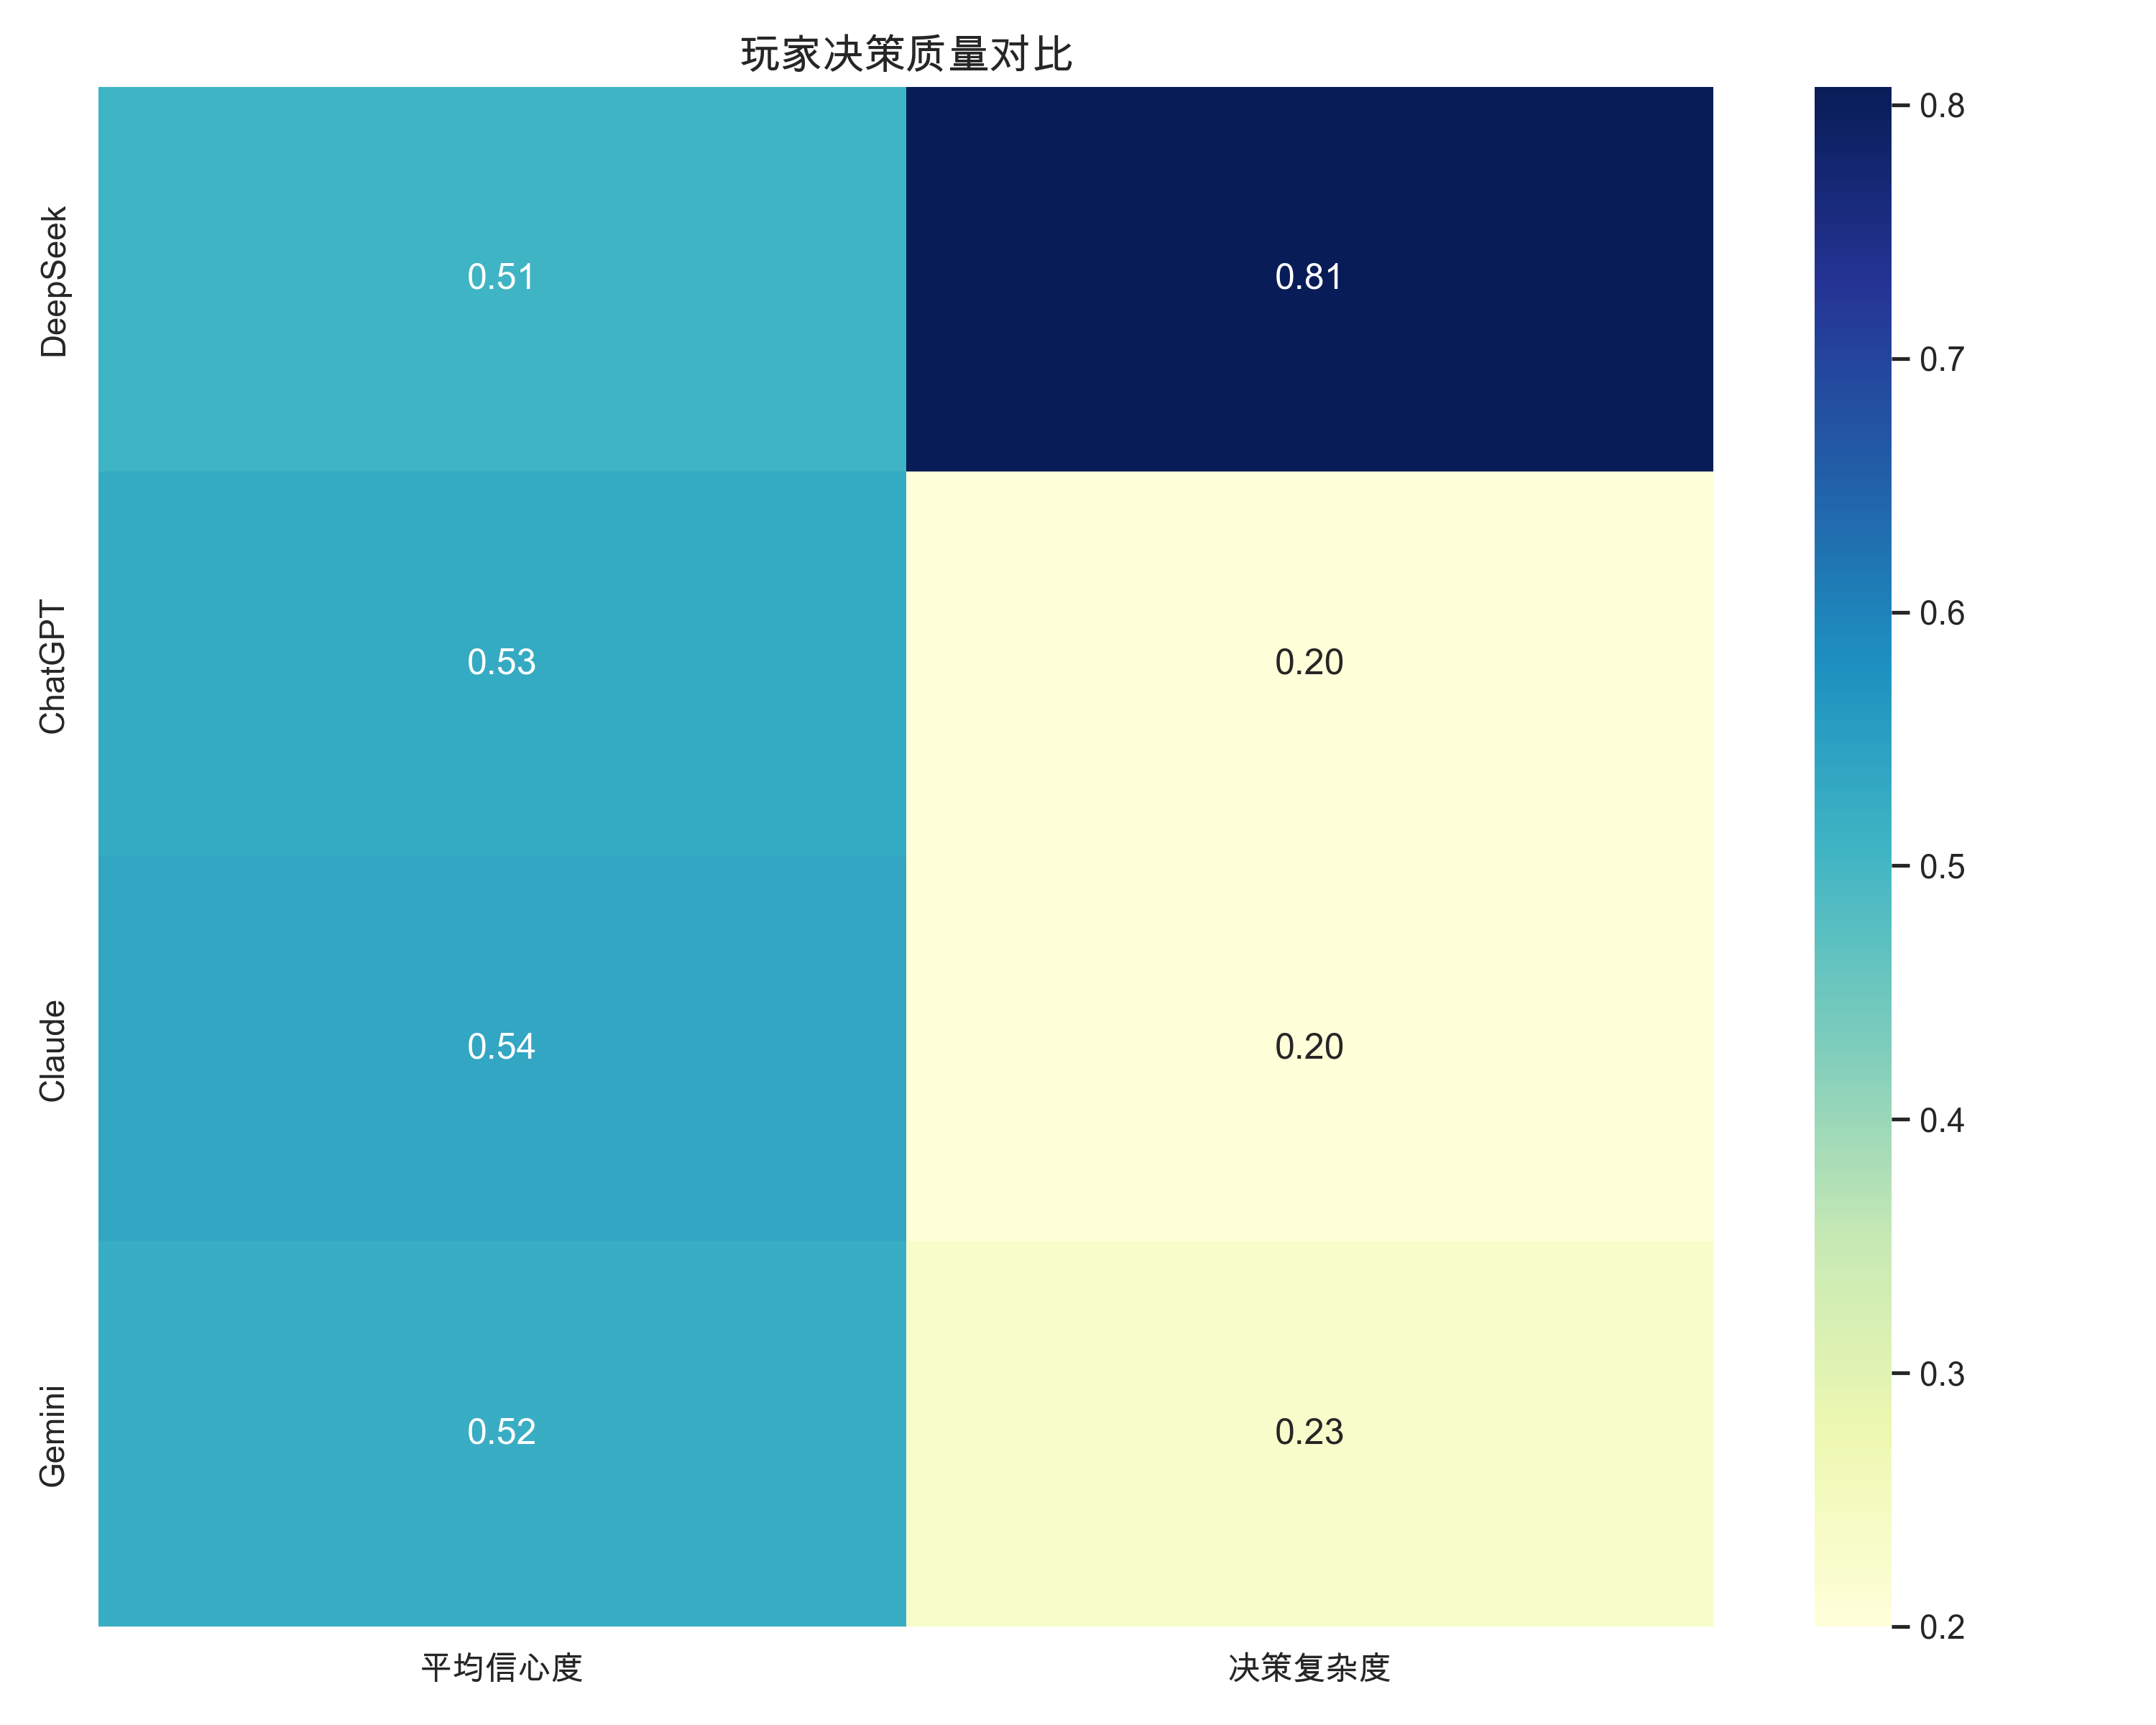
\includegraphics[width=0.9\textwidth]{figures/player_decision_quality_comparison.png}
    \caption{Comprehensive comparison of decision quality metrics across the four LLM models}
    \label{fig:decision_quality_comparison}
\end{figure}

The evolution of strategic behaviors over time is captured in Figures \ref{fig:bluff_trend} and \ref{fig:challenge_trend}, which show how the models' bluffing and challenging rates changed throughout the tournament.

\begin{figure}[H]
    \centering
    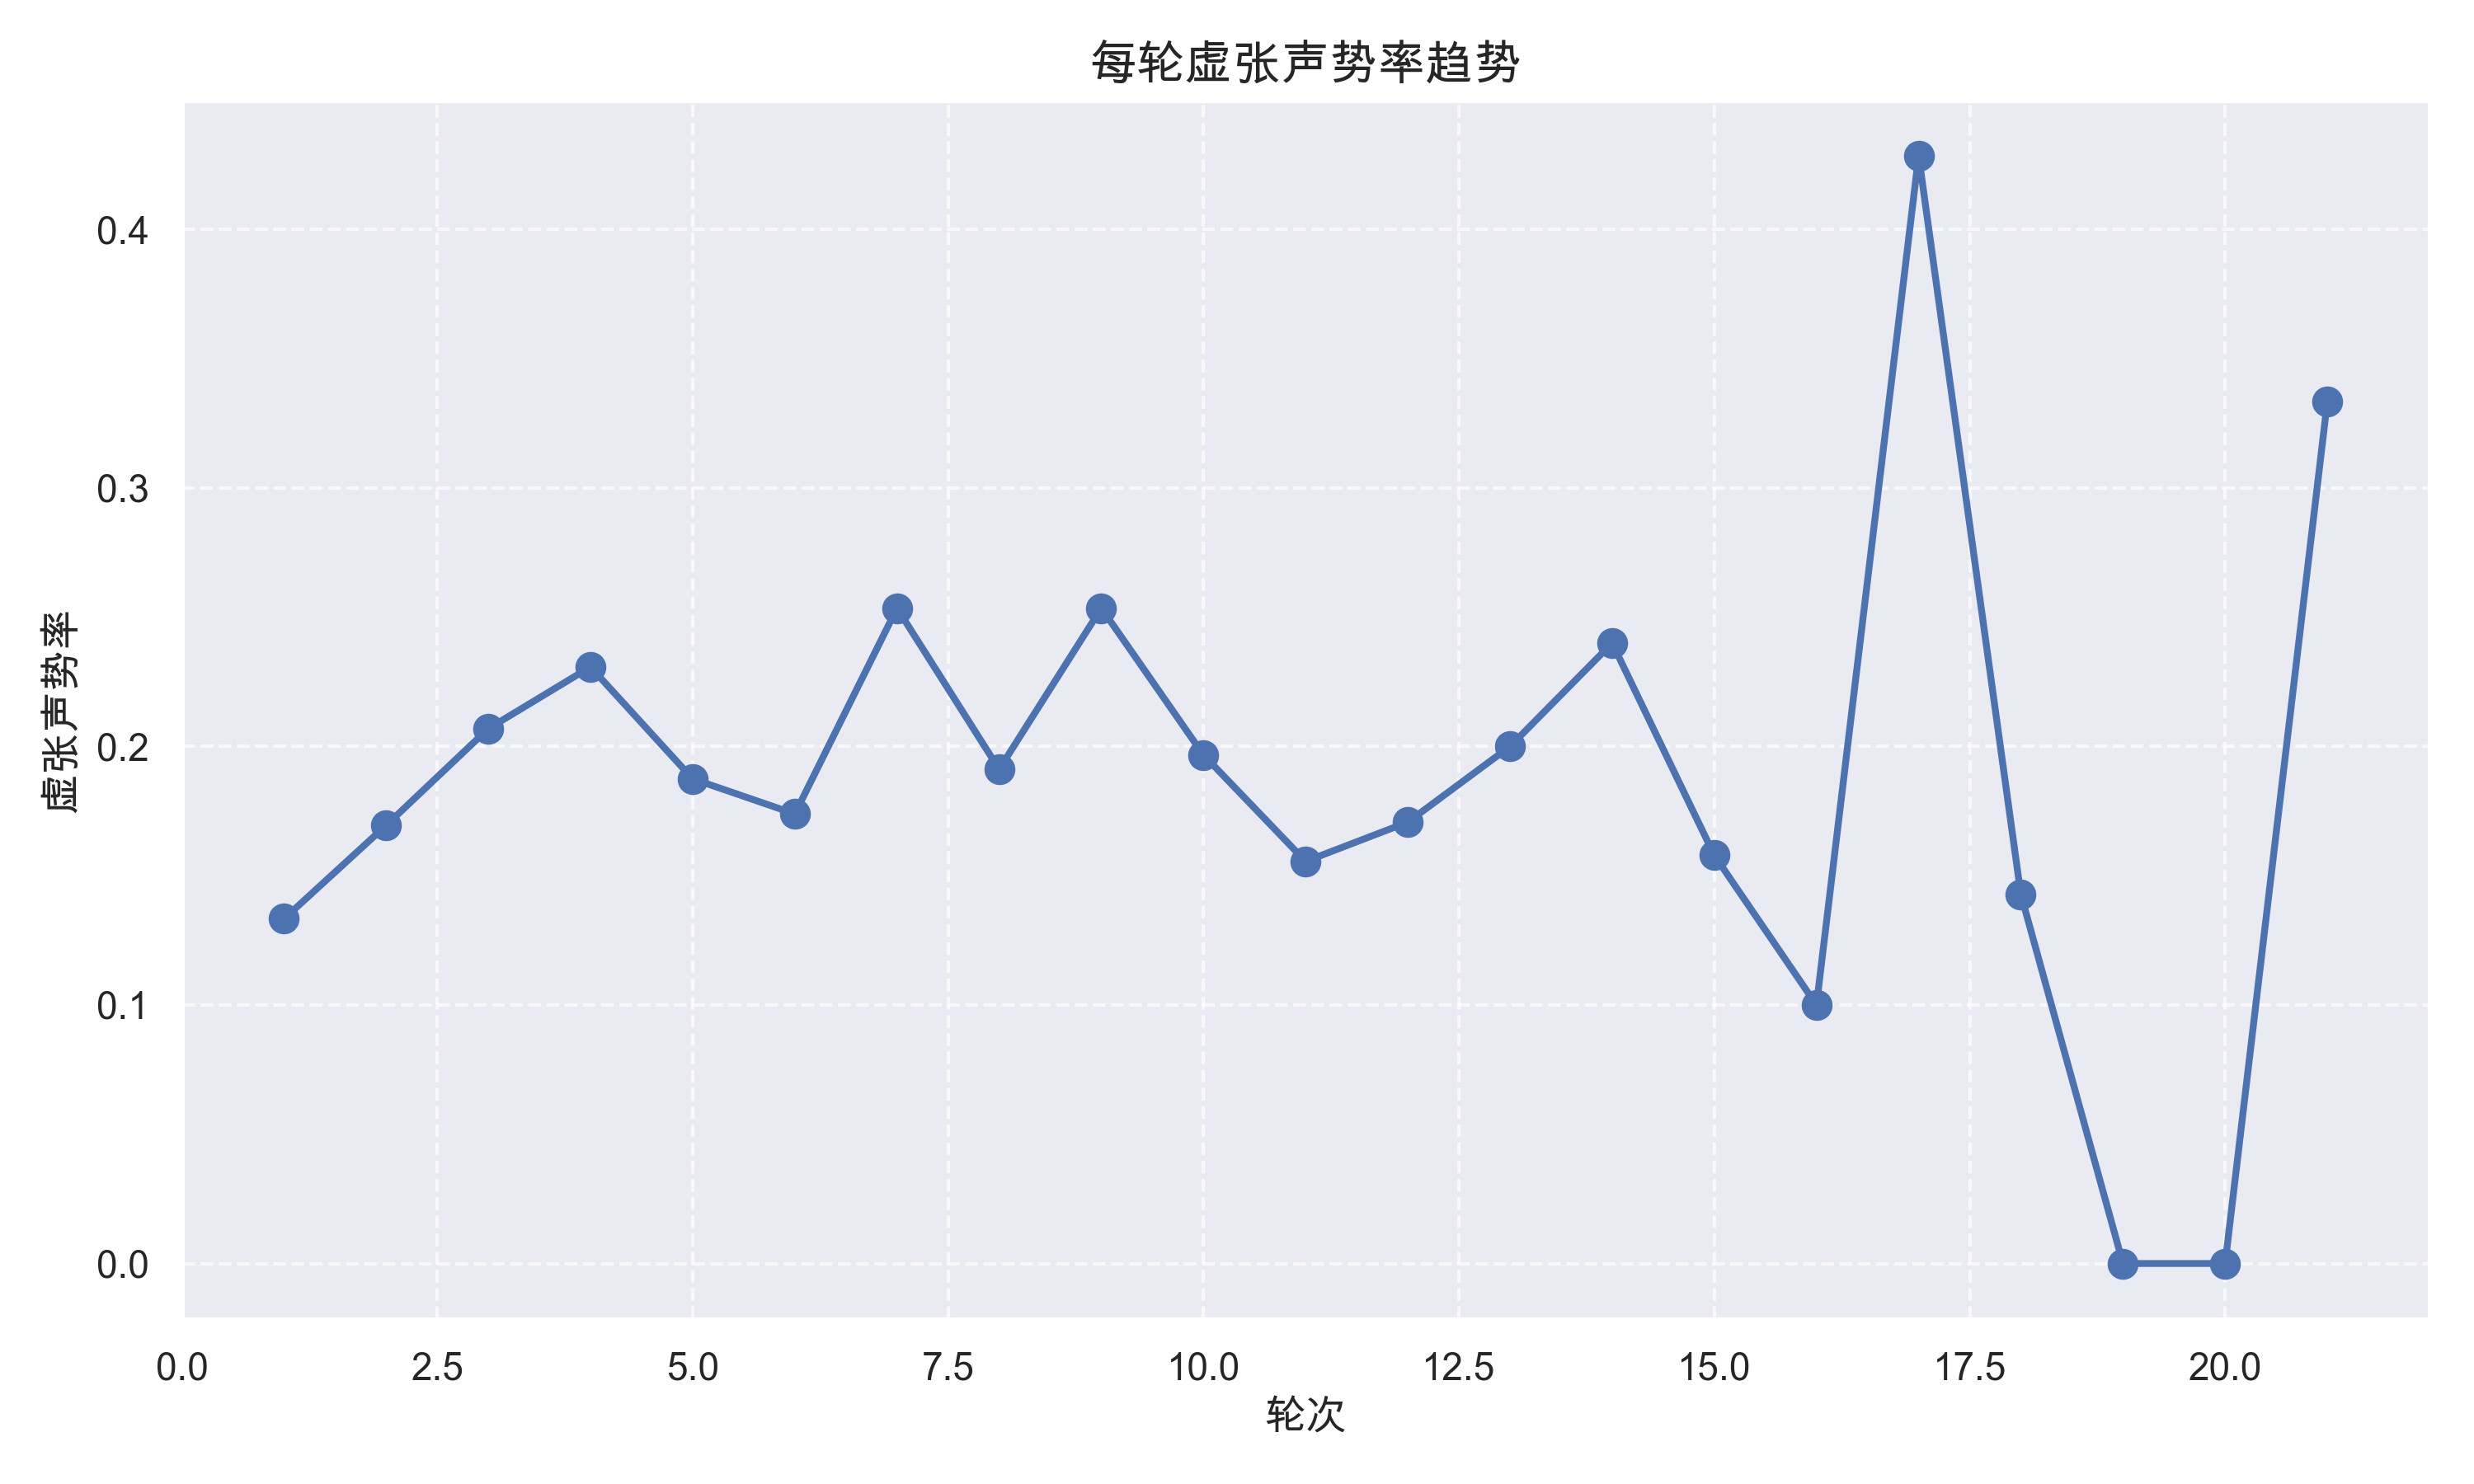
\includegraphics[width=0.9\textwidth]{figures/bluff_rate_trend.png}
    \caption{Bluff rate trends showing the evolution of deceptive strategies over multiple game rounds}
    \label{fig:bluff_trend}
\end{figure}

\begin{figure}[H]
    \centering
    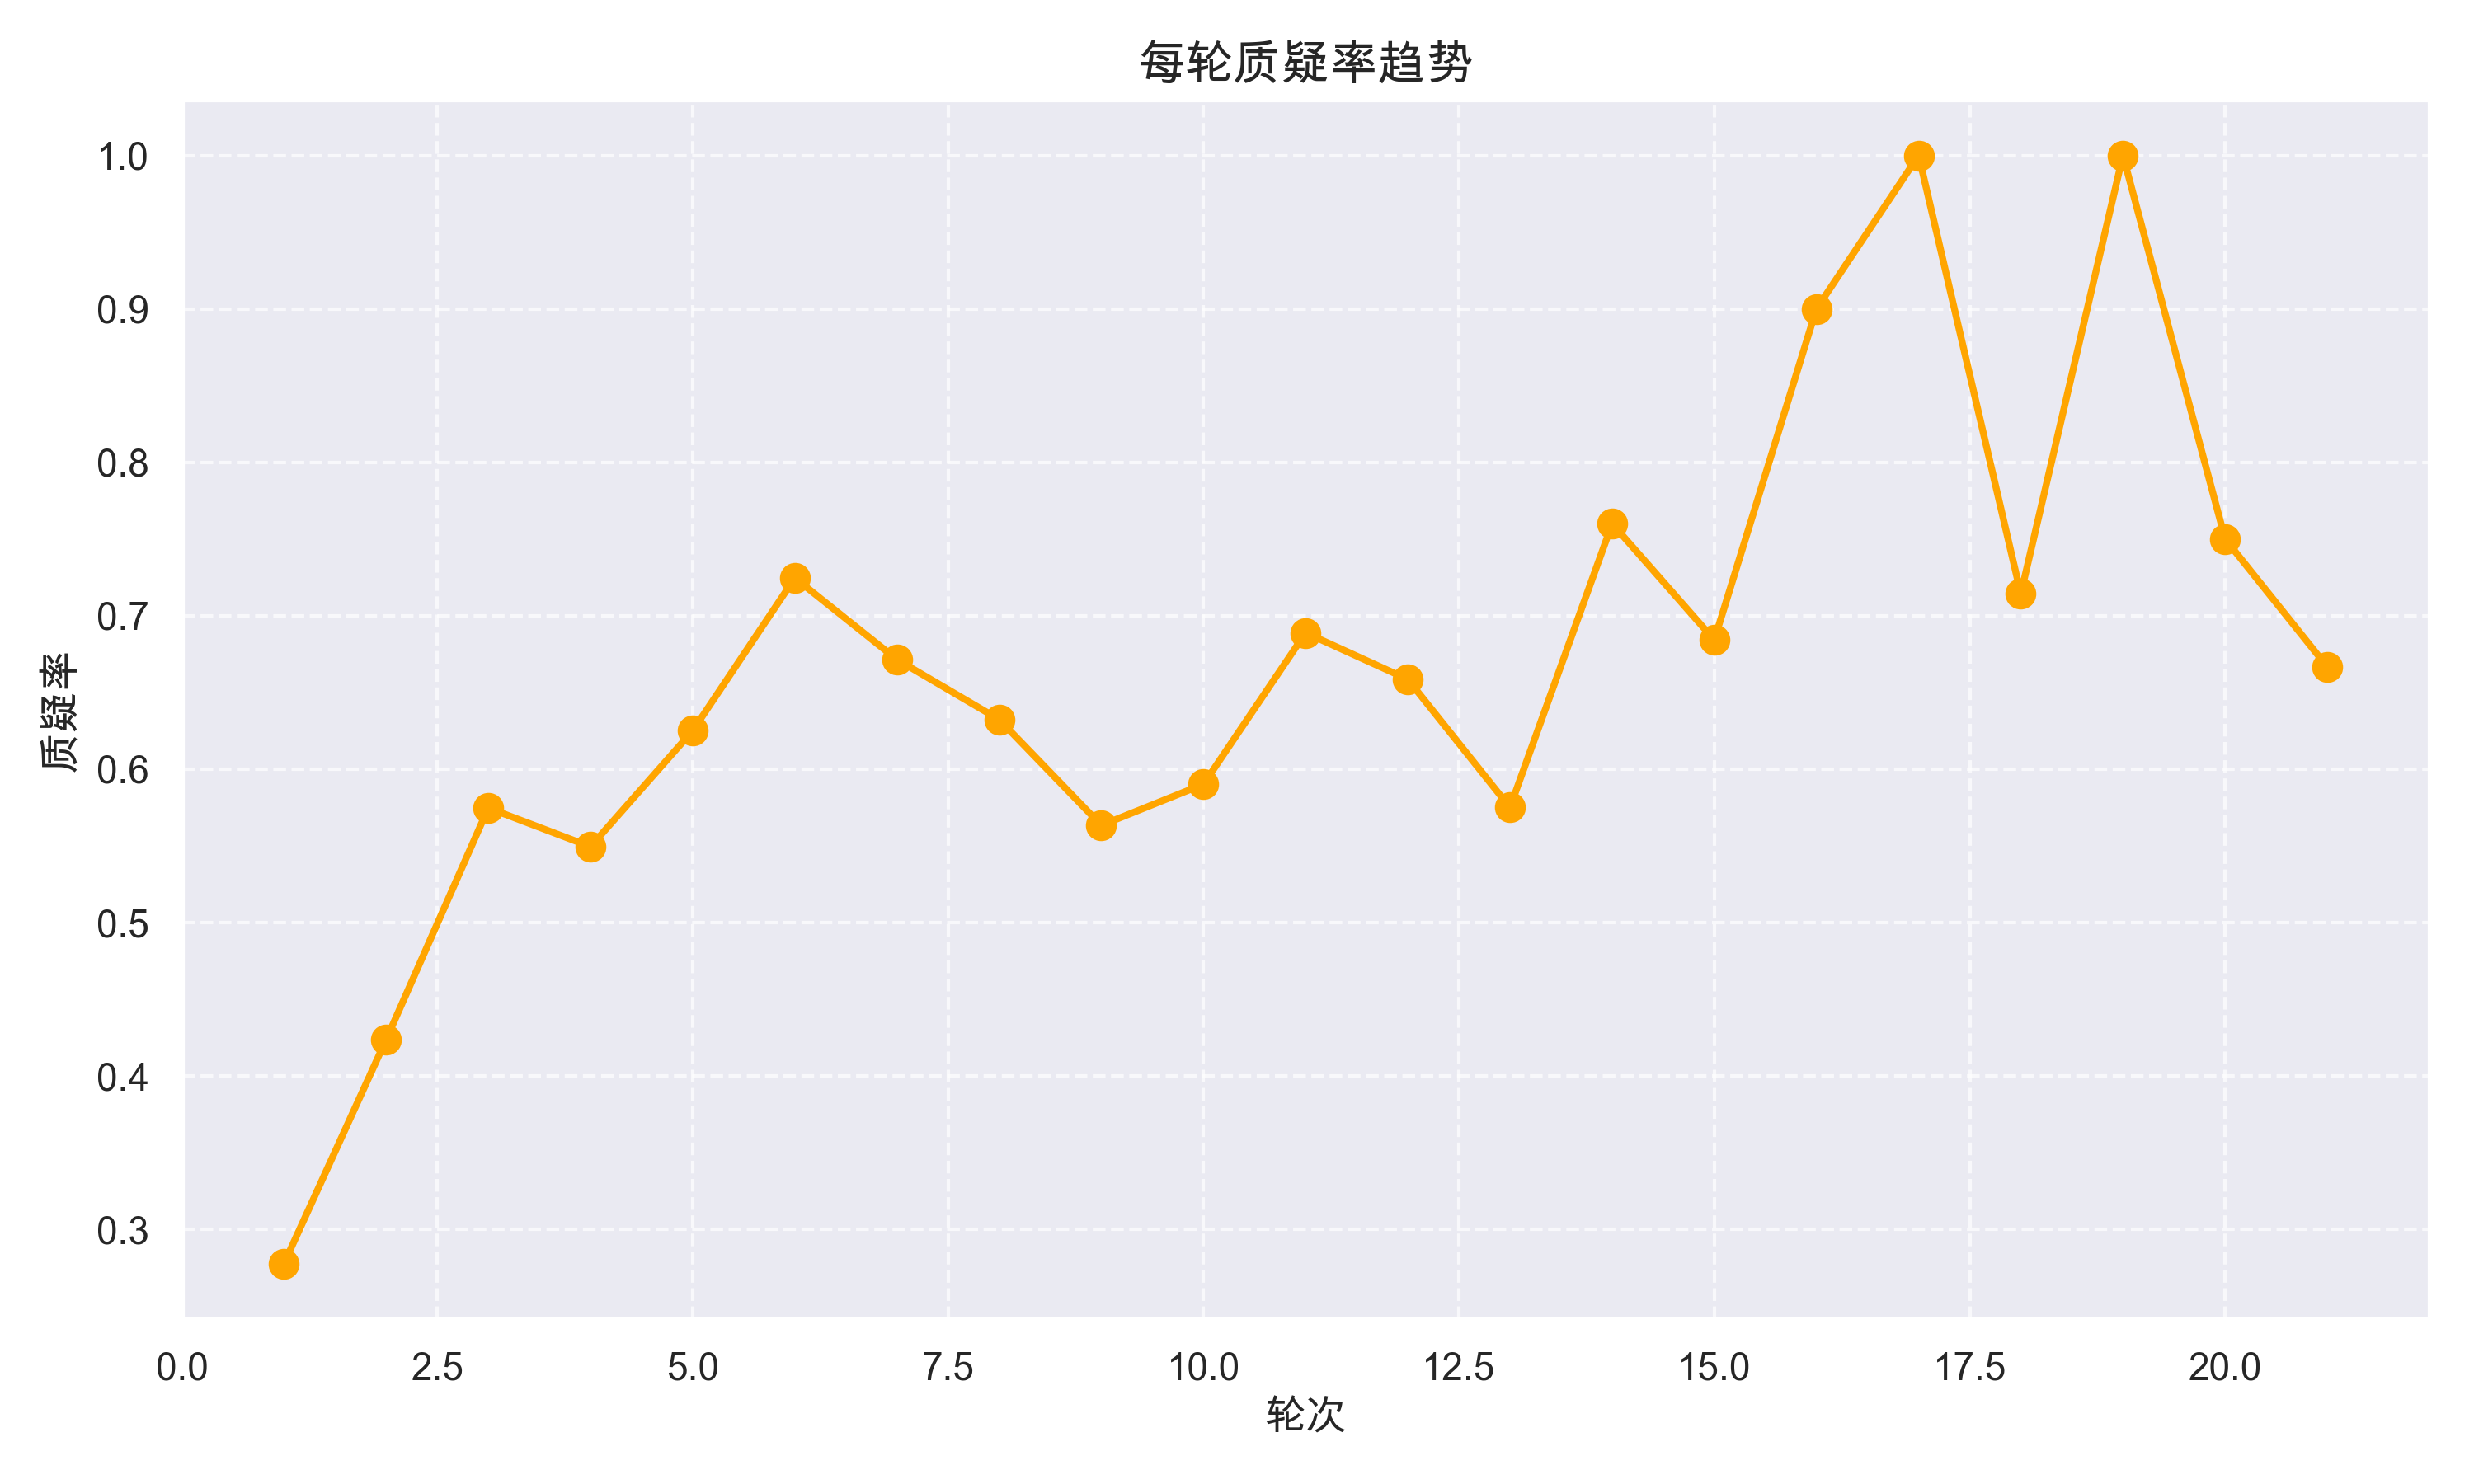
\includegraphics[width=0.9\textwidth]{figures/challenge_rate_trend.png}
    \caption{Challenge rate trends revealing patterns in skepticism and risk assessment behaviors}
    \label{fig:challenge_trend}
\end{figure}

\subsubsection{Card Efficiency}
Card efficiency analysis revealed:
\begin{itemize}
    \item \textbf{Strategic Card Usage:} DeepSeek and Claude demonstrated the most efficient use of cards relative to game outcomes (efficiency scores of 1.88 and 1.84 respectively).
    \item \textbf{Target Card Conservation:} Models with higher survival rates showed better conservation of target cards for critical game situations.
\end{itemize}

These efficiency metrics are quantified in Figure \ref{fig:card_efficiency}, demonstrating significant differences in how models utilized their available cards.

\begin{figure}[H]
    \centering
    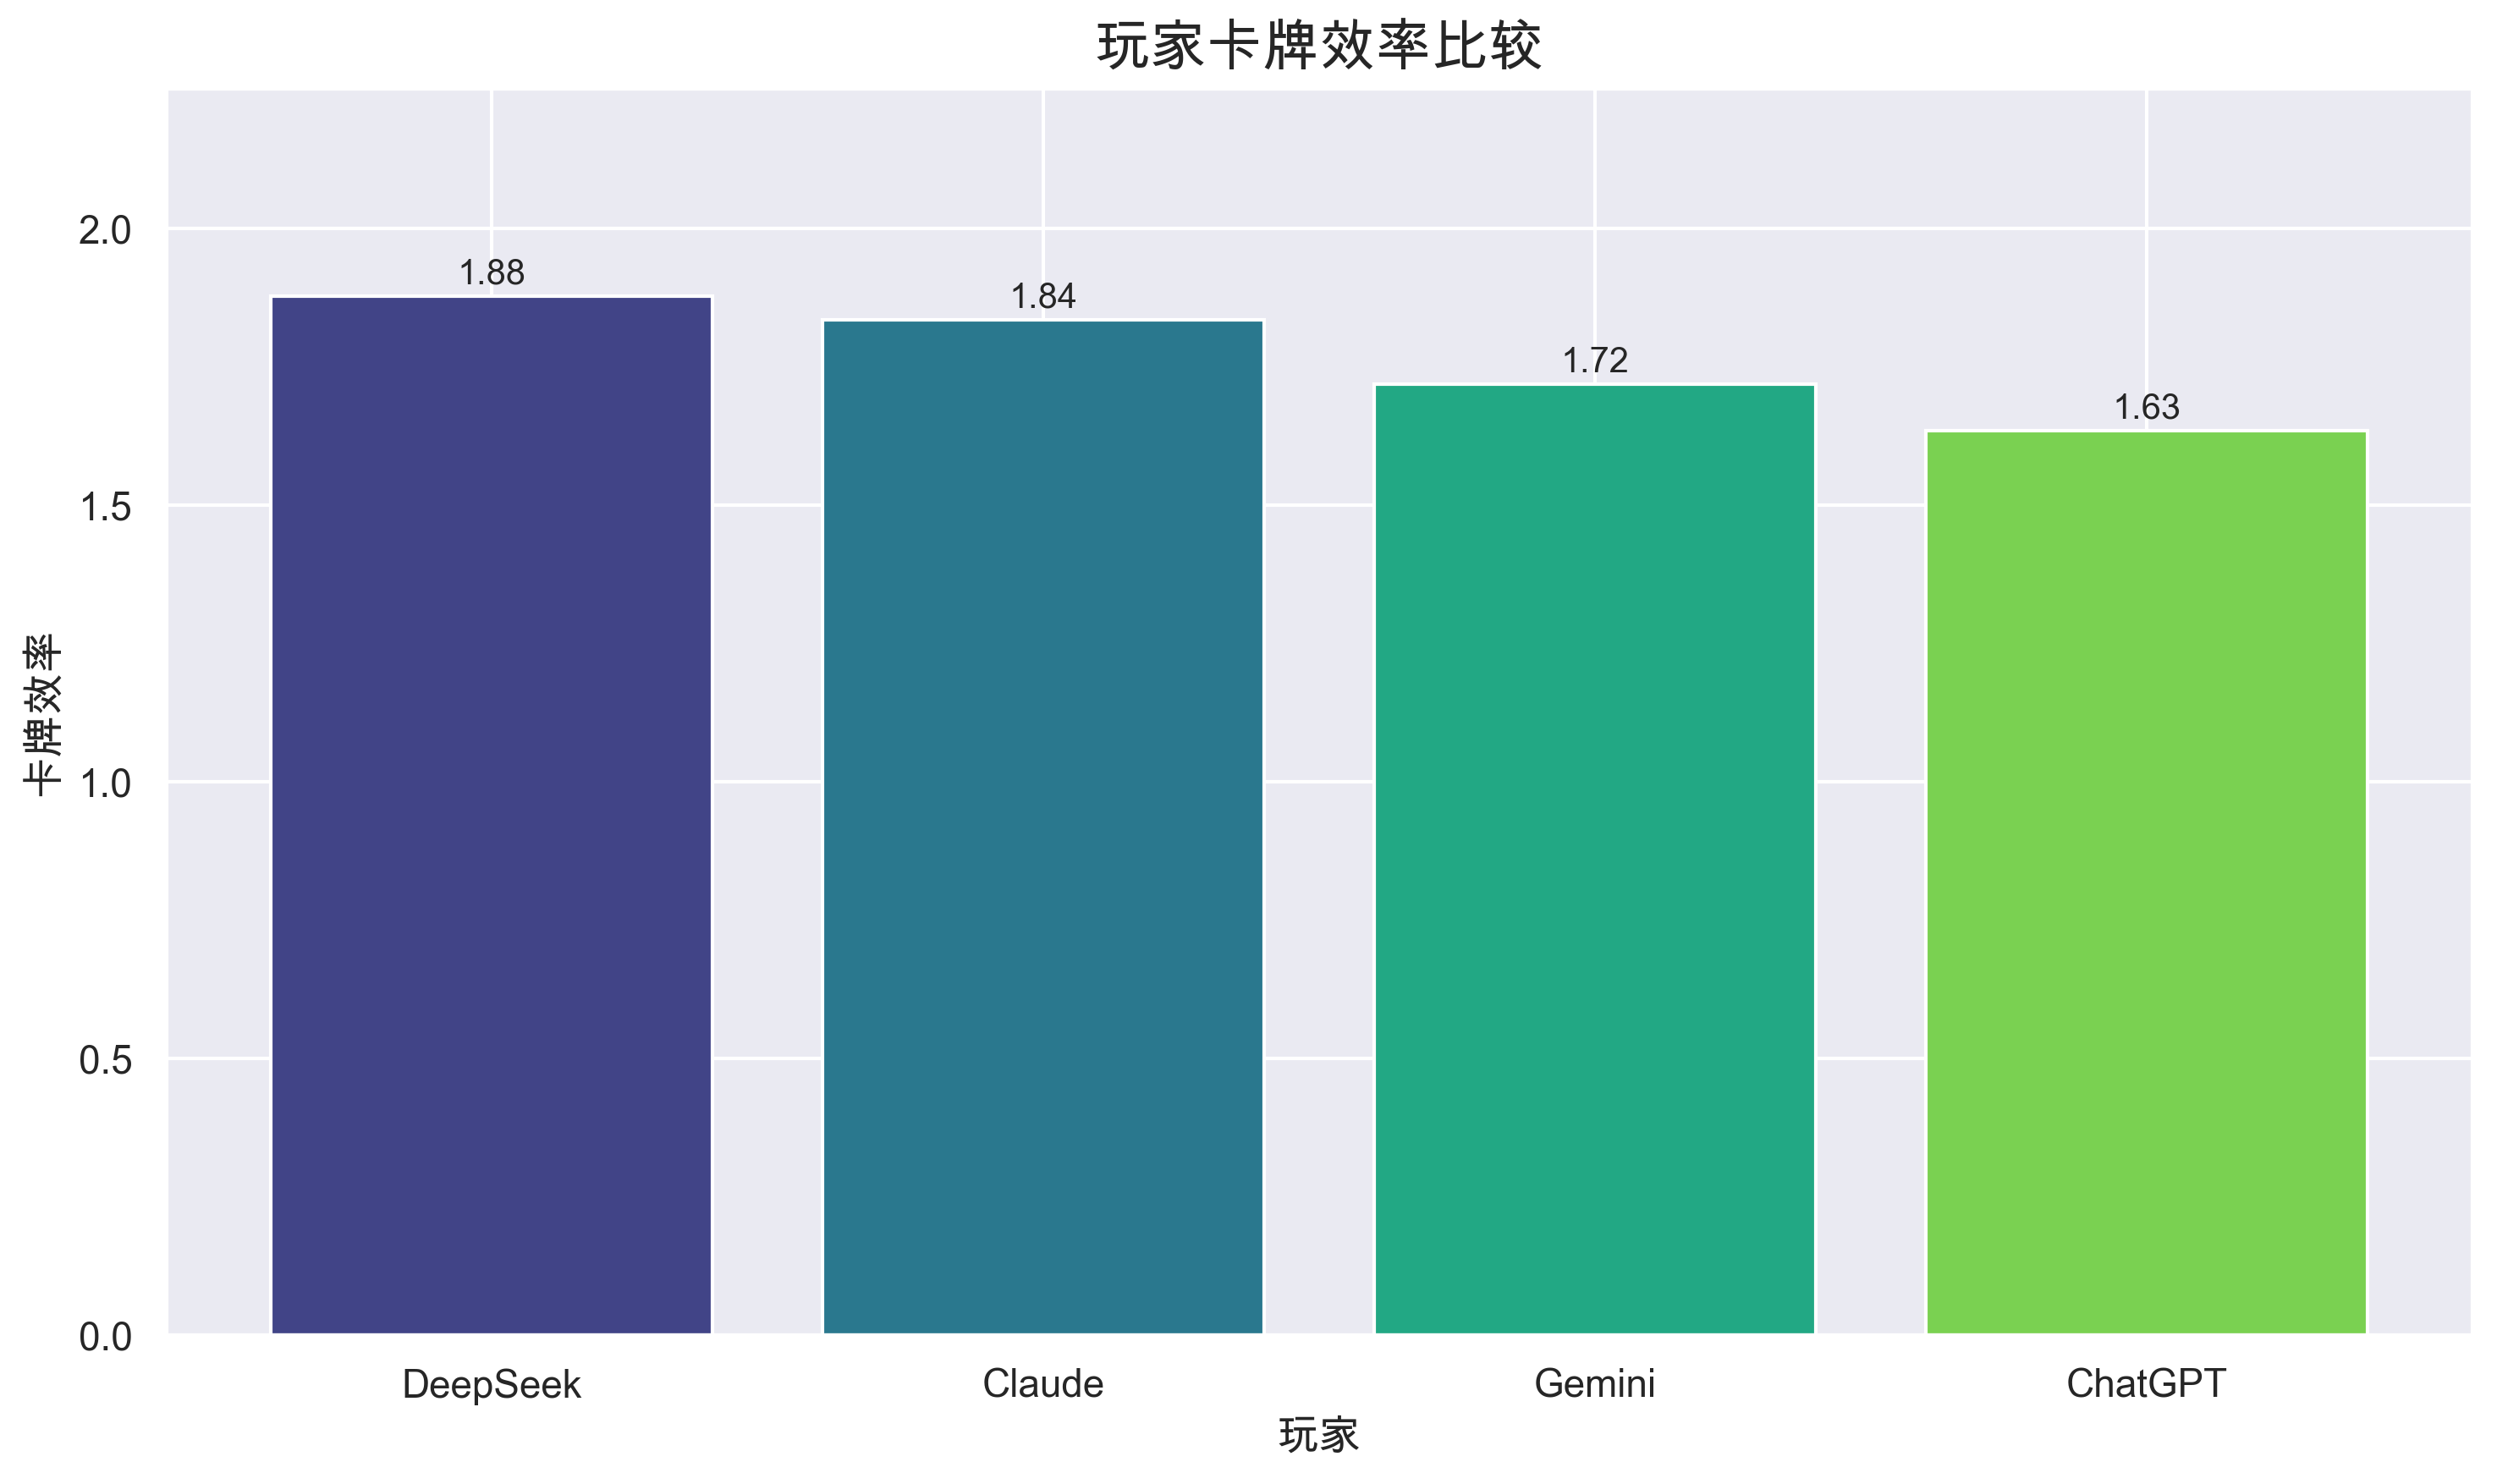
\includegraphics[width=0.9\textwidth]{figures/decision_card_efficiency.png}
    \caption{Card efficiency scores showing effectiveness of card usage relative to game outcomes}
    \label{fig:card_efficiency}
\end{figure}

Figures \ref{fig:top_models_decision_radar} and \ref{fig:other_models_decision_radar} present detailed decision radar charts that visualize the distinct decision-making patterns of each model pair, highlighting the strategic similarities and differences between the top performers (DeepSeek and Claude) and the other models (ChatGPT and Gemini).

\begin{figure}[H]
    \centering
    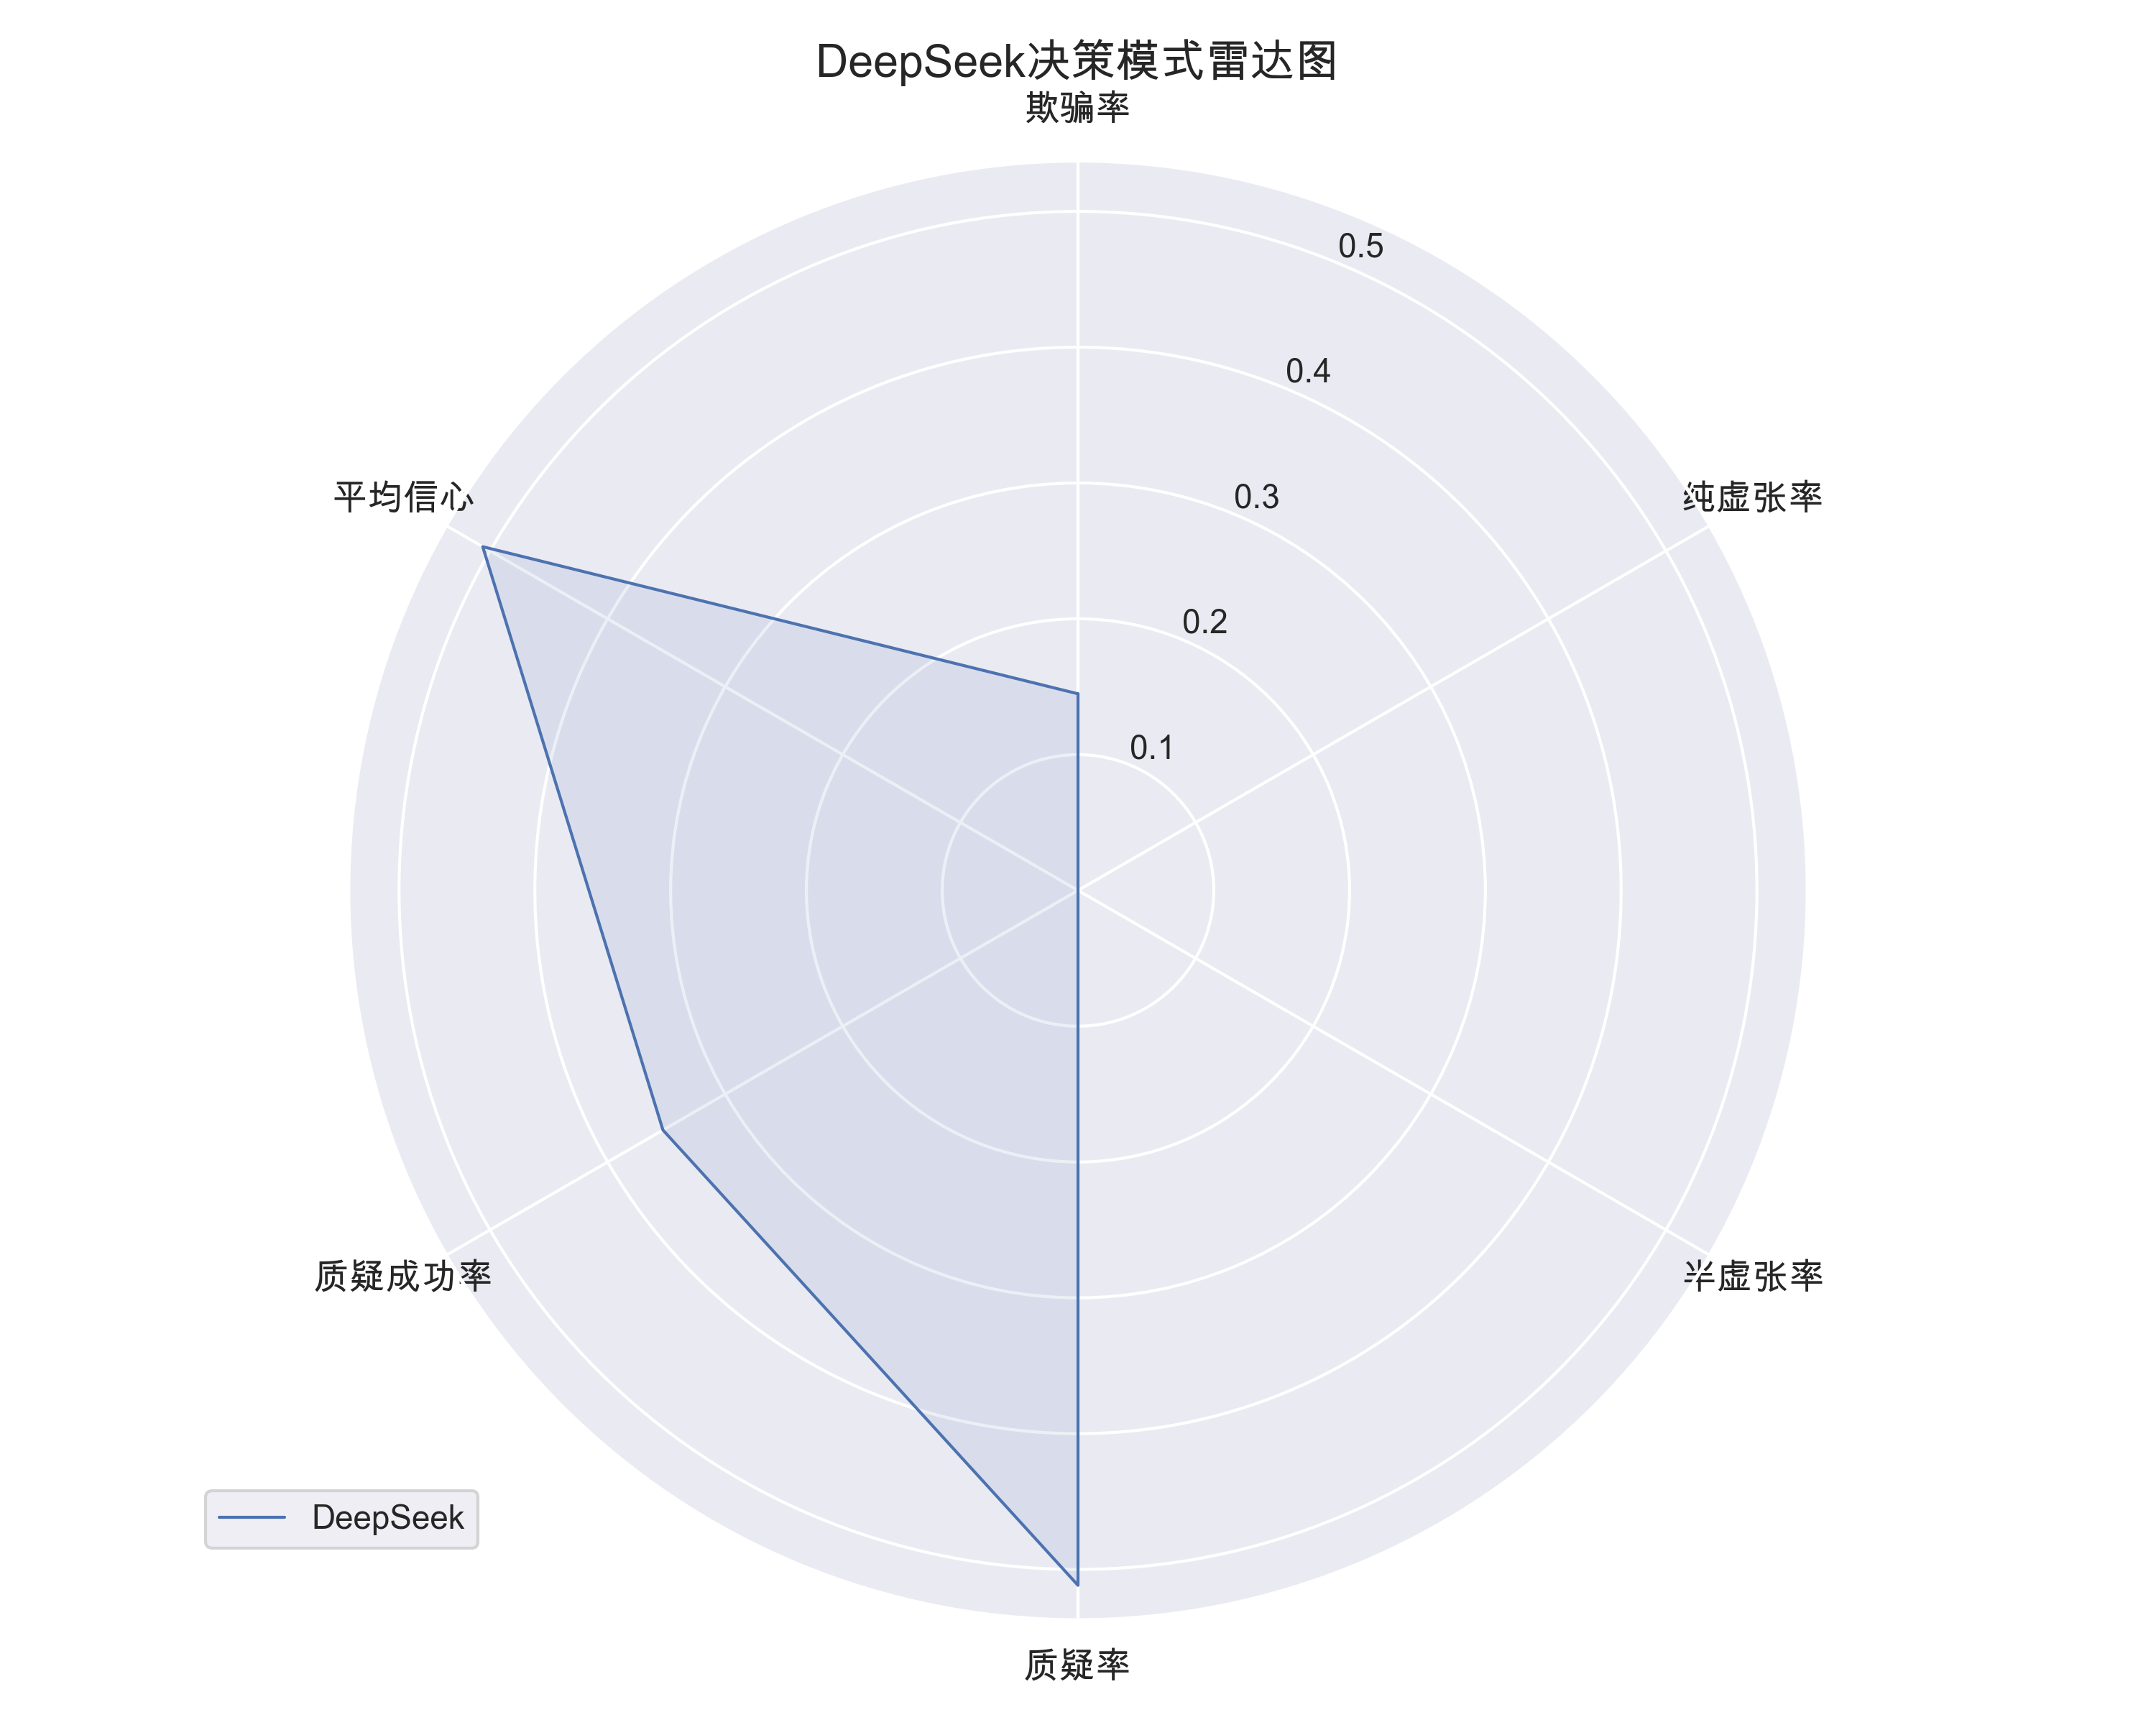
\includegraphics[width=0.45\textwidth]{figures/DeepSeek_decision_radar.png}
    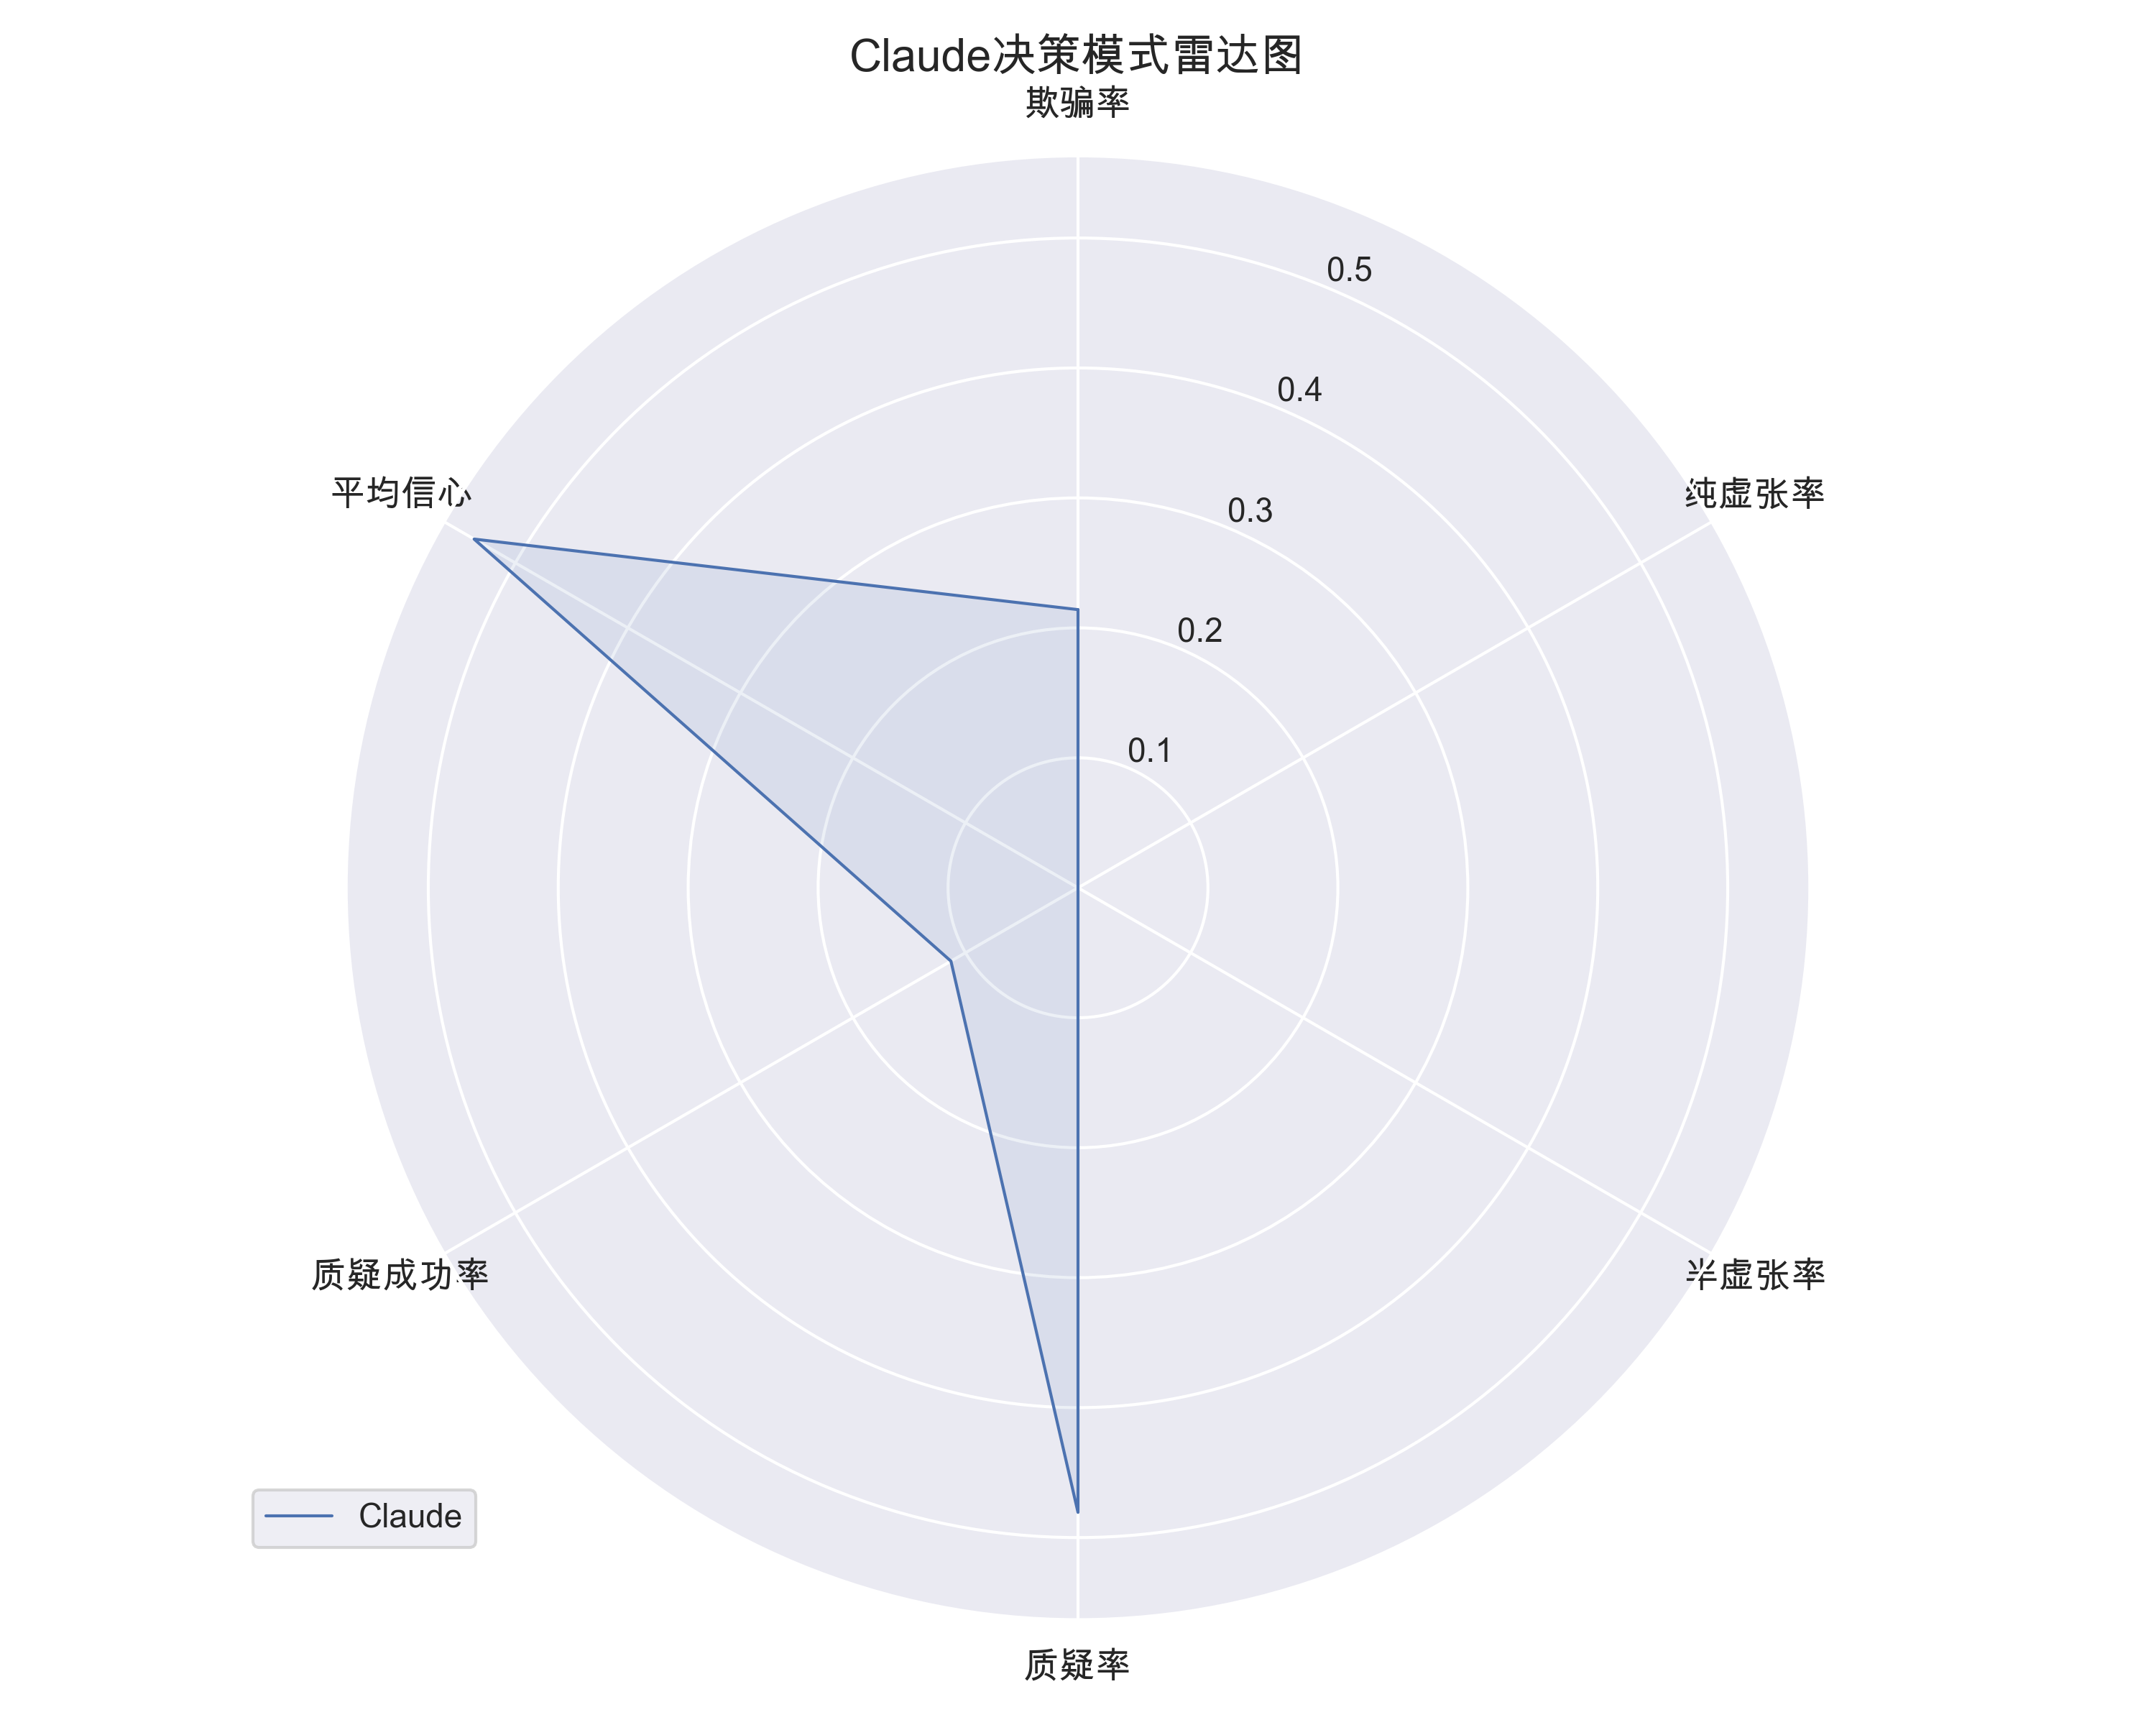
\includegraphics[width=0.45\textwidth]{figures/Claude_decision_radar.png}
    \caption{Decision radar charts for DeepSeek (left) and Claude (right) showing distinct decision-making patterns}
    \label{fig:top_models_decision_radar}
\end{figure}

\begin{figure}[H]
    \centering
    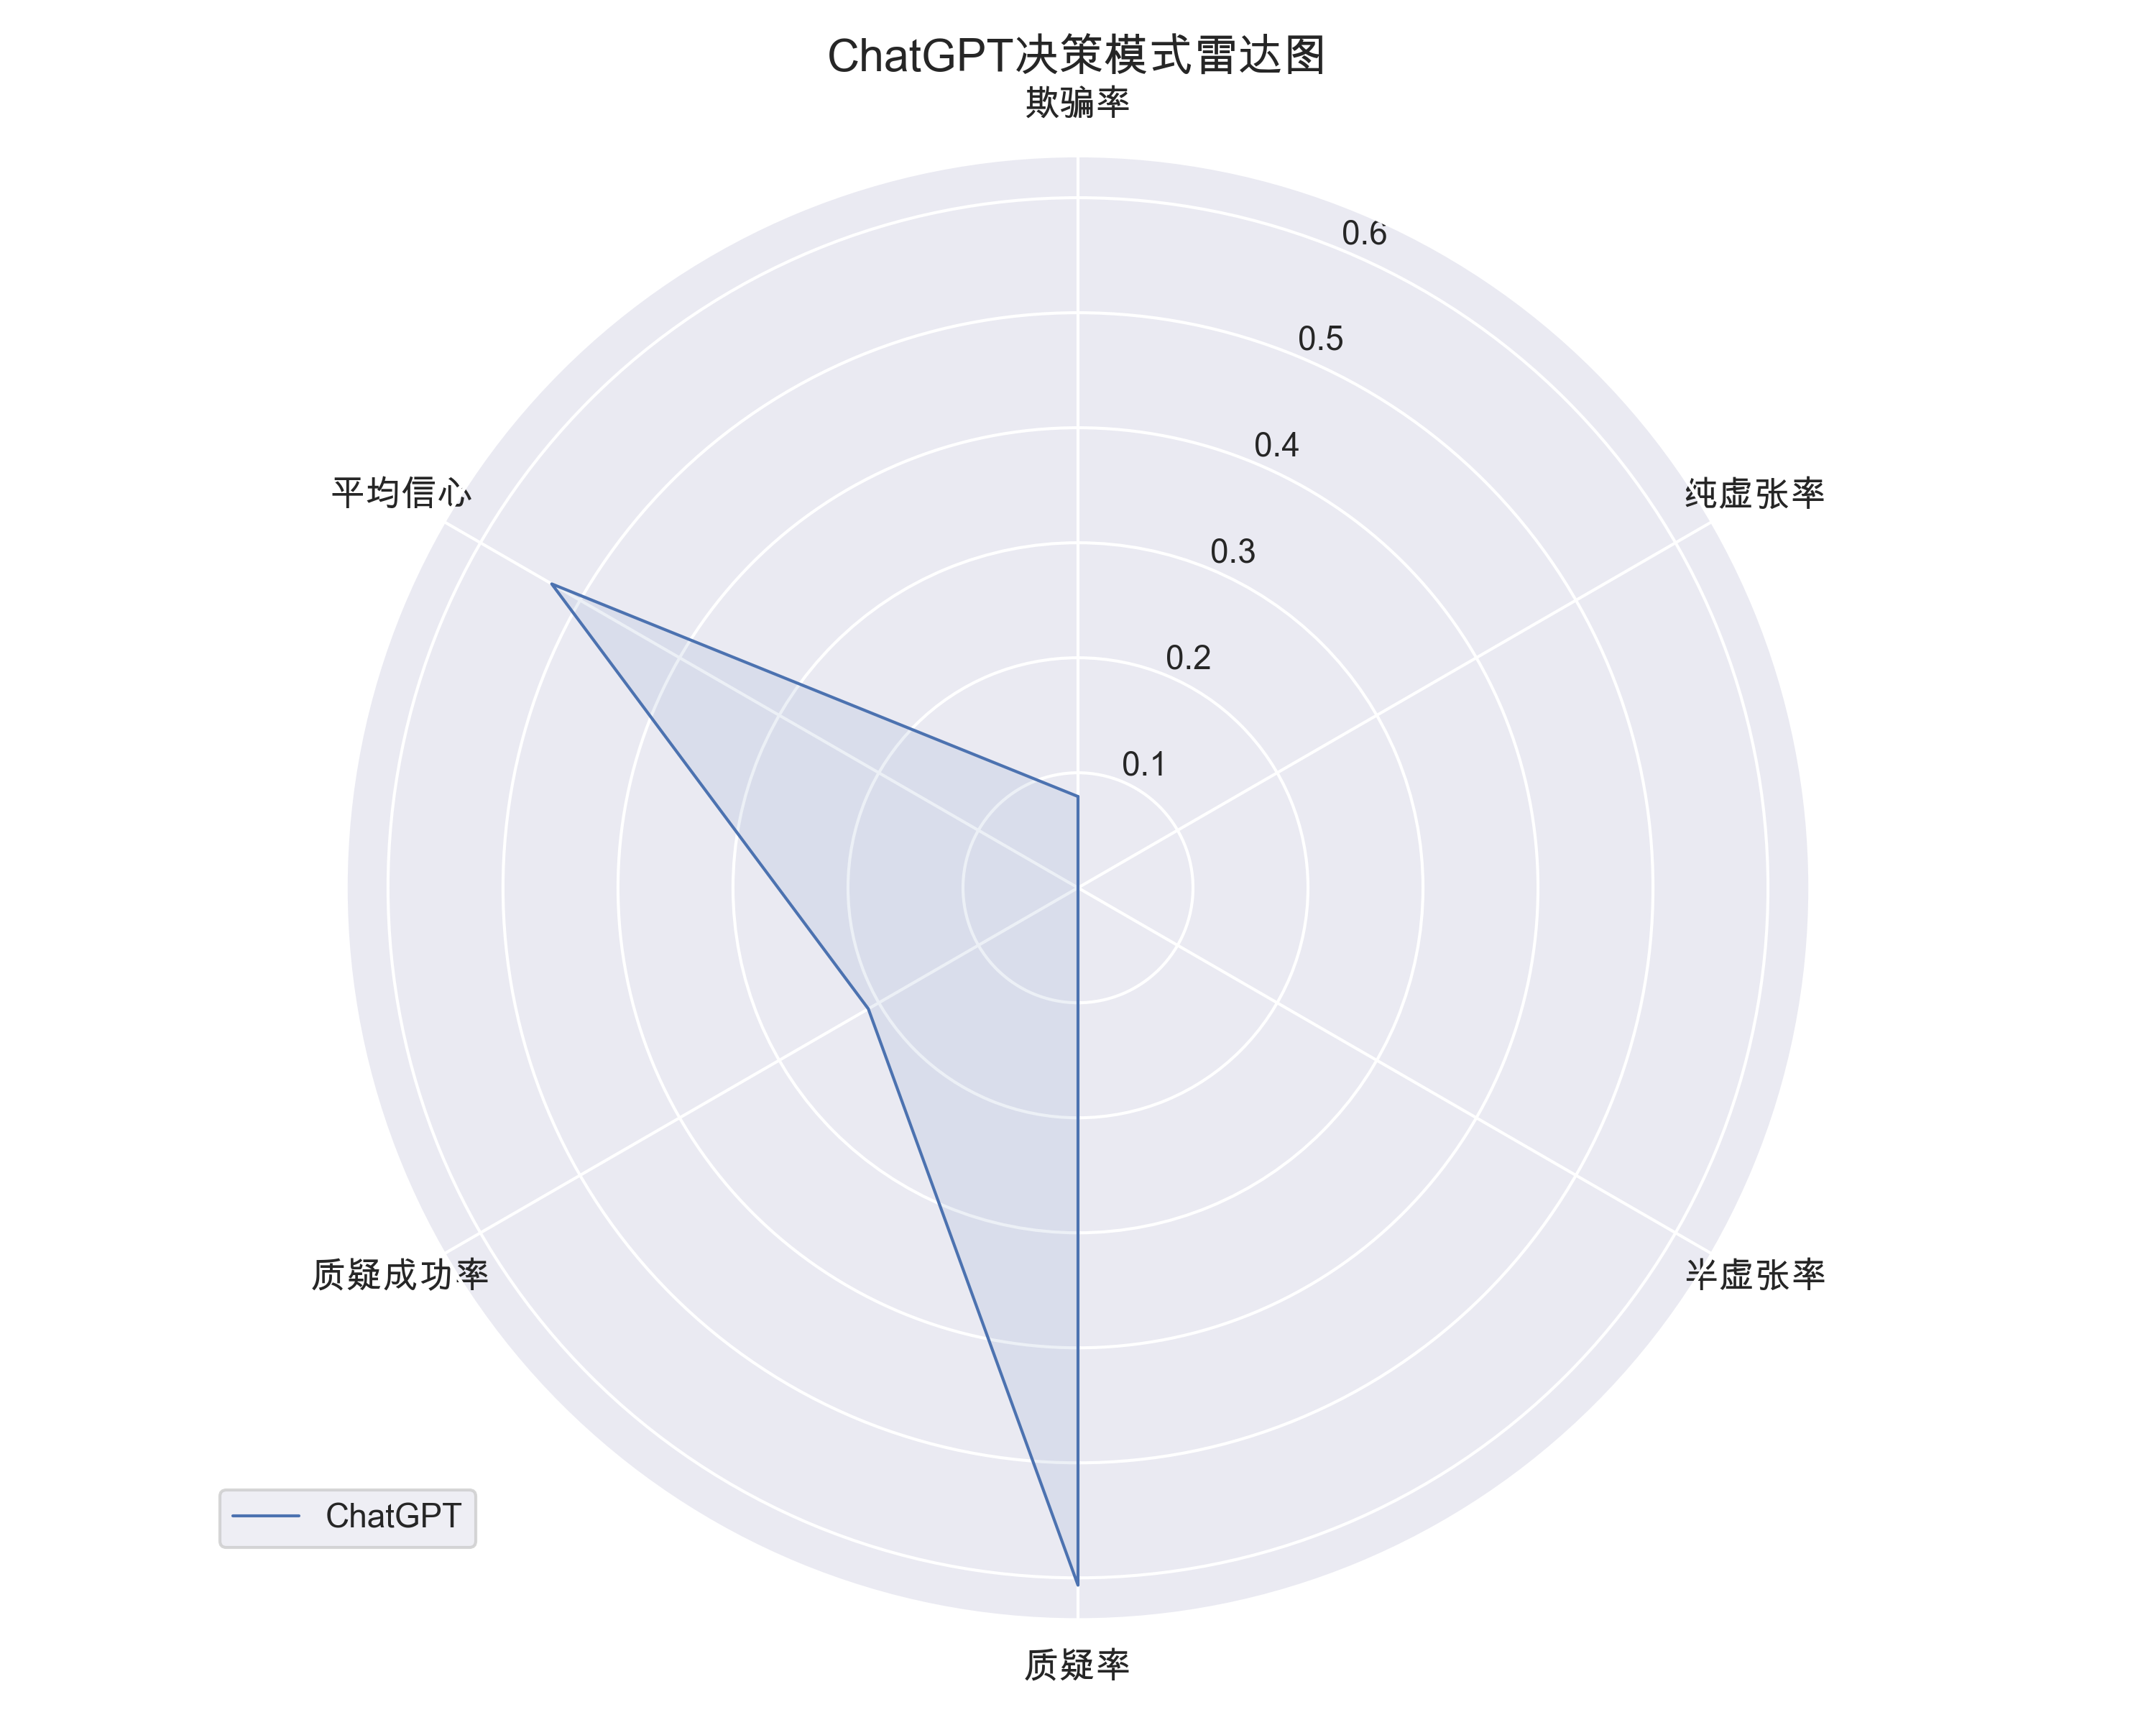
\includegraphics[width=0.45\textwidth]{figures/ChatGPT_decision_radar.png}
    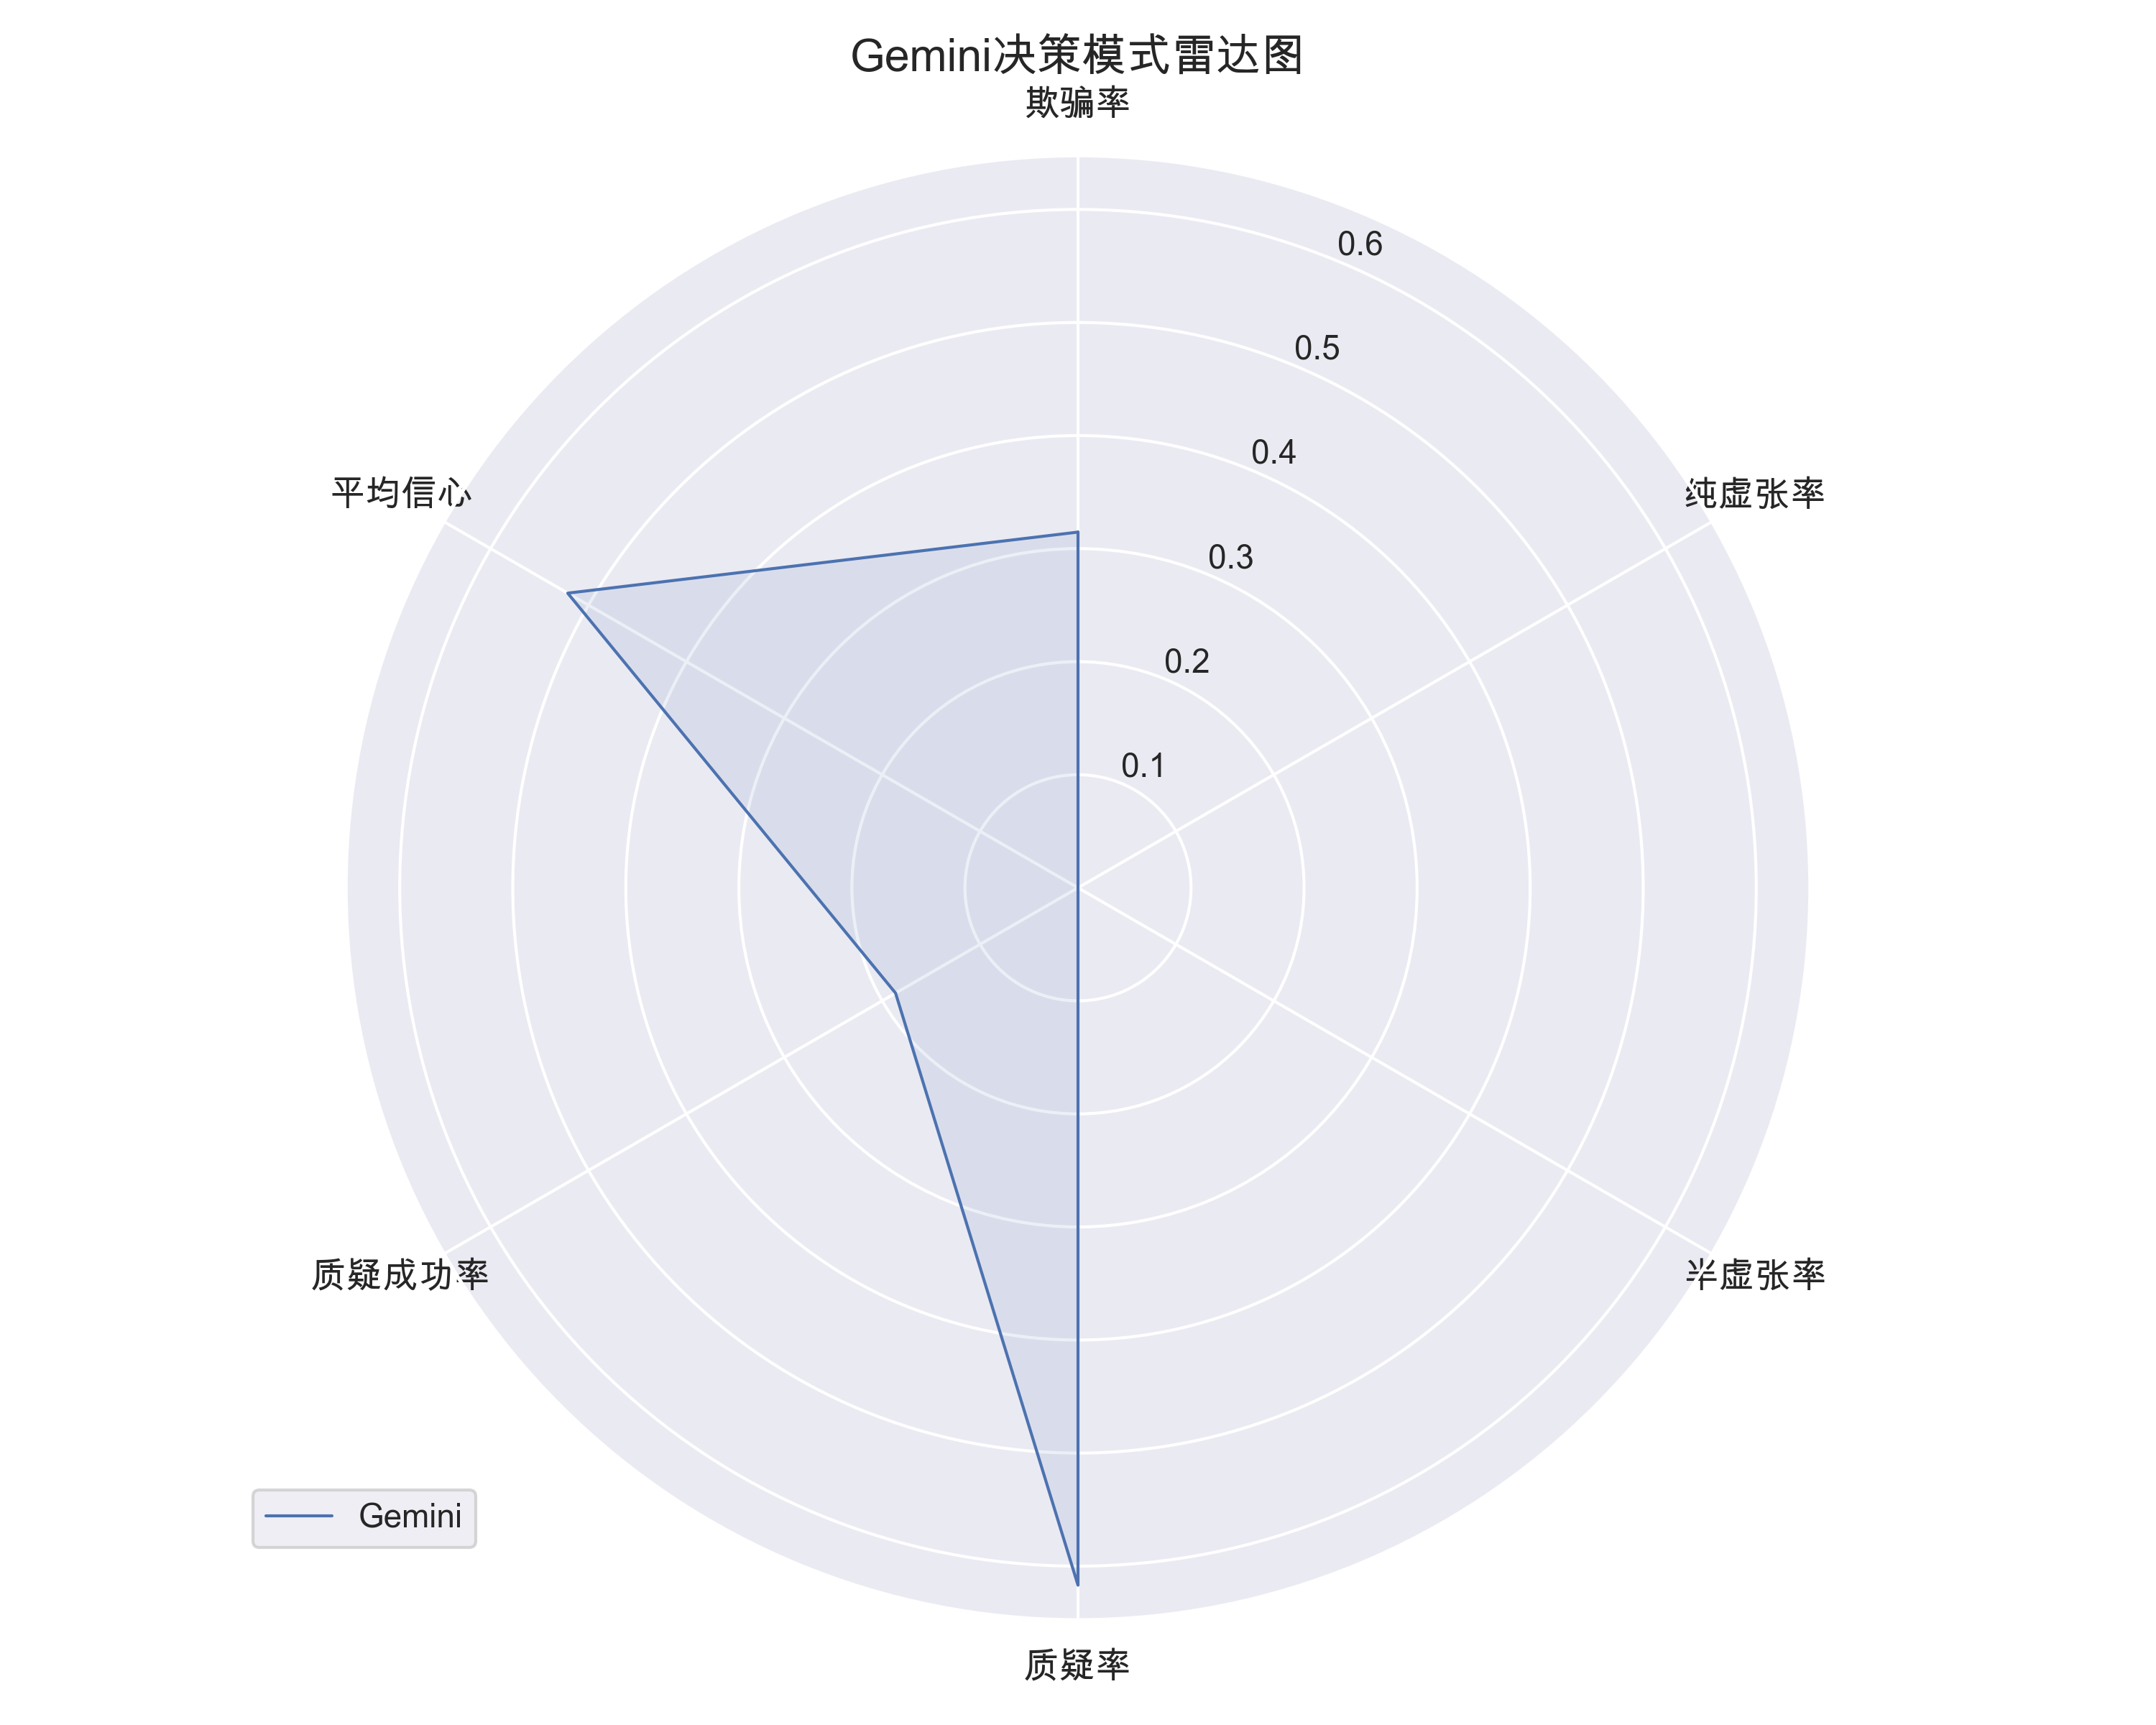
\includegraphics[width=0.45\textwidth]{figures/Gemini_decision_radar.png}
    \caption{Decision radar charts for ChatGPT (left) and Gemini (right) revealing contrasting decision strategies}
    \label{fig:other_models_decision_radar}
\end{figure}

\subsection{Strategic Behavior Patterns}
Through cluster analysis of gameplay patterns, we identified four distinct strategic profiles among the LLM agents. Figure \ref{fig:emotion_confidence} illustrates the relationship between emotional states and decision confidence across game progression.

\begin{figure}[H]
    \centering
    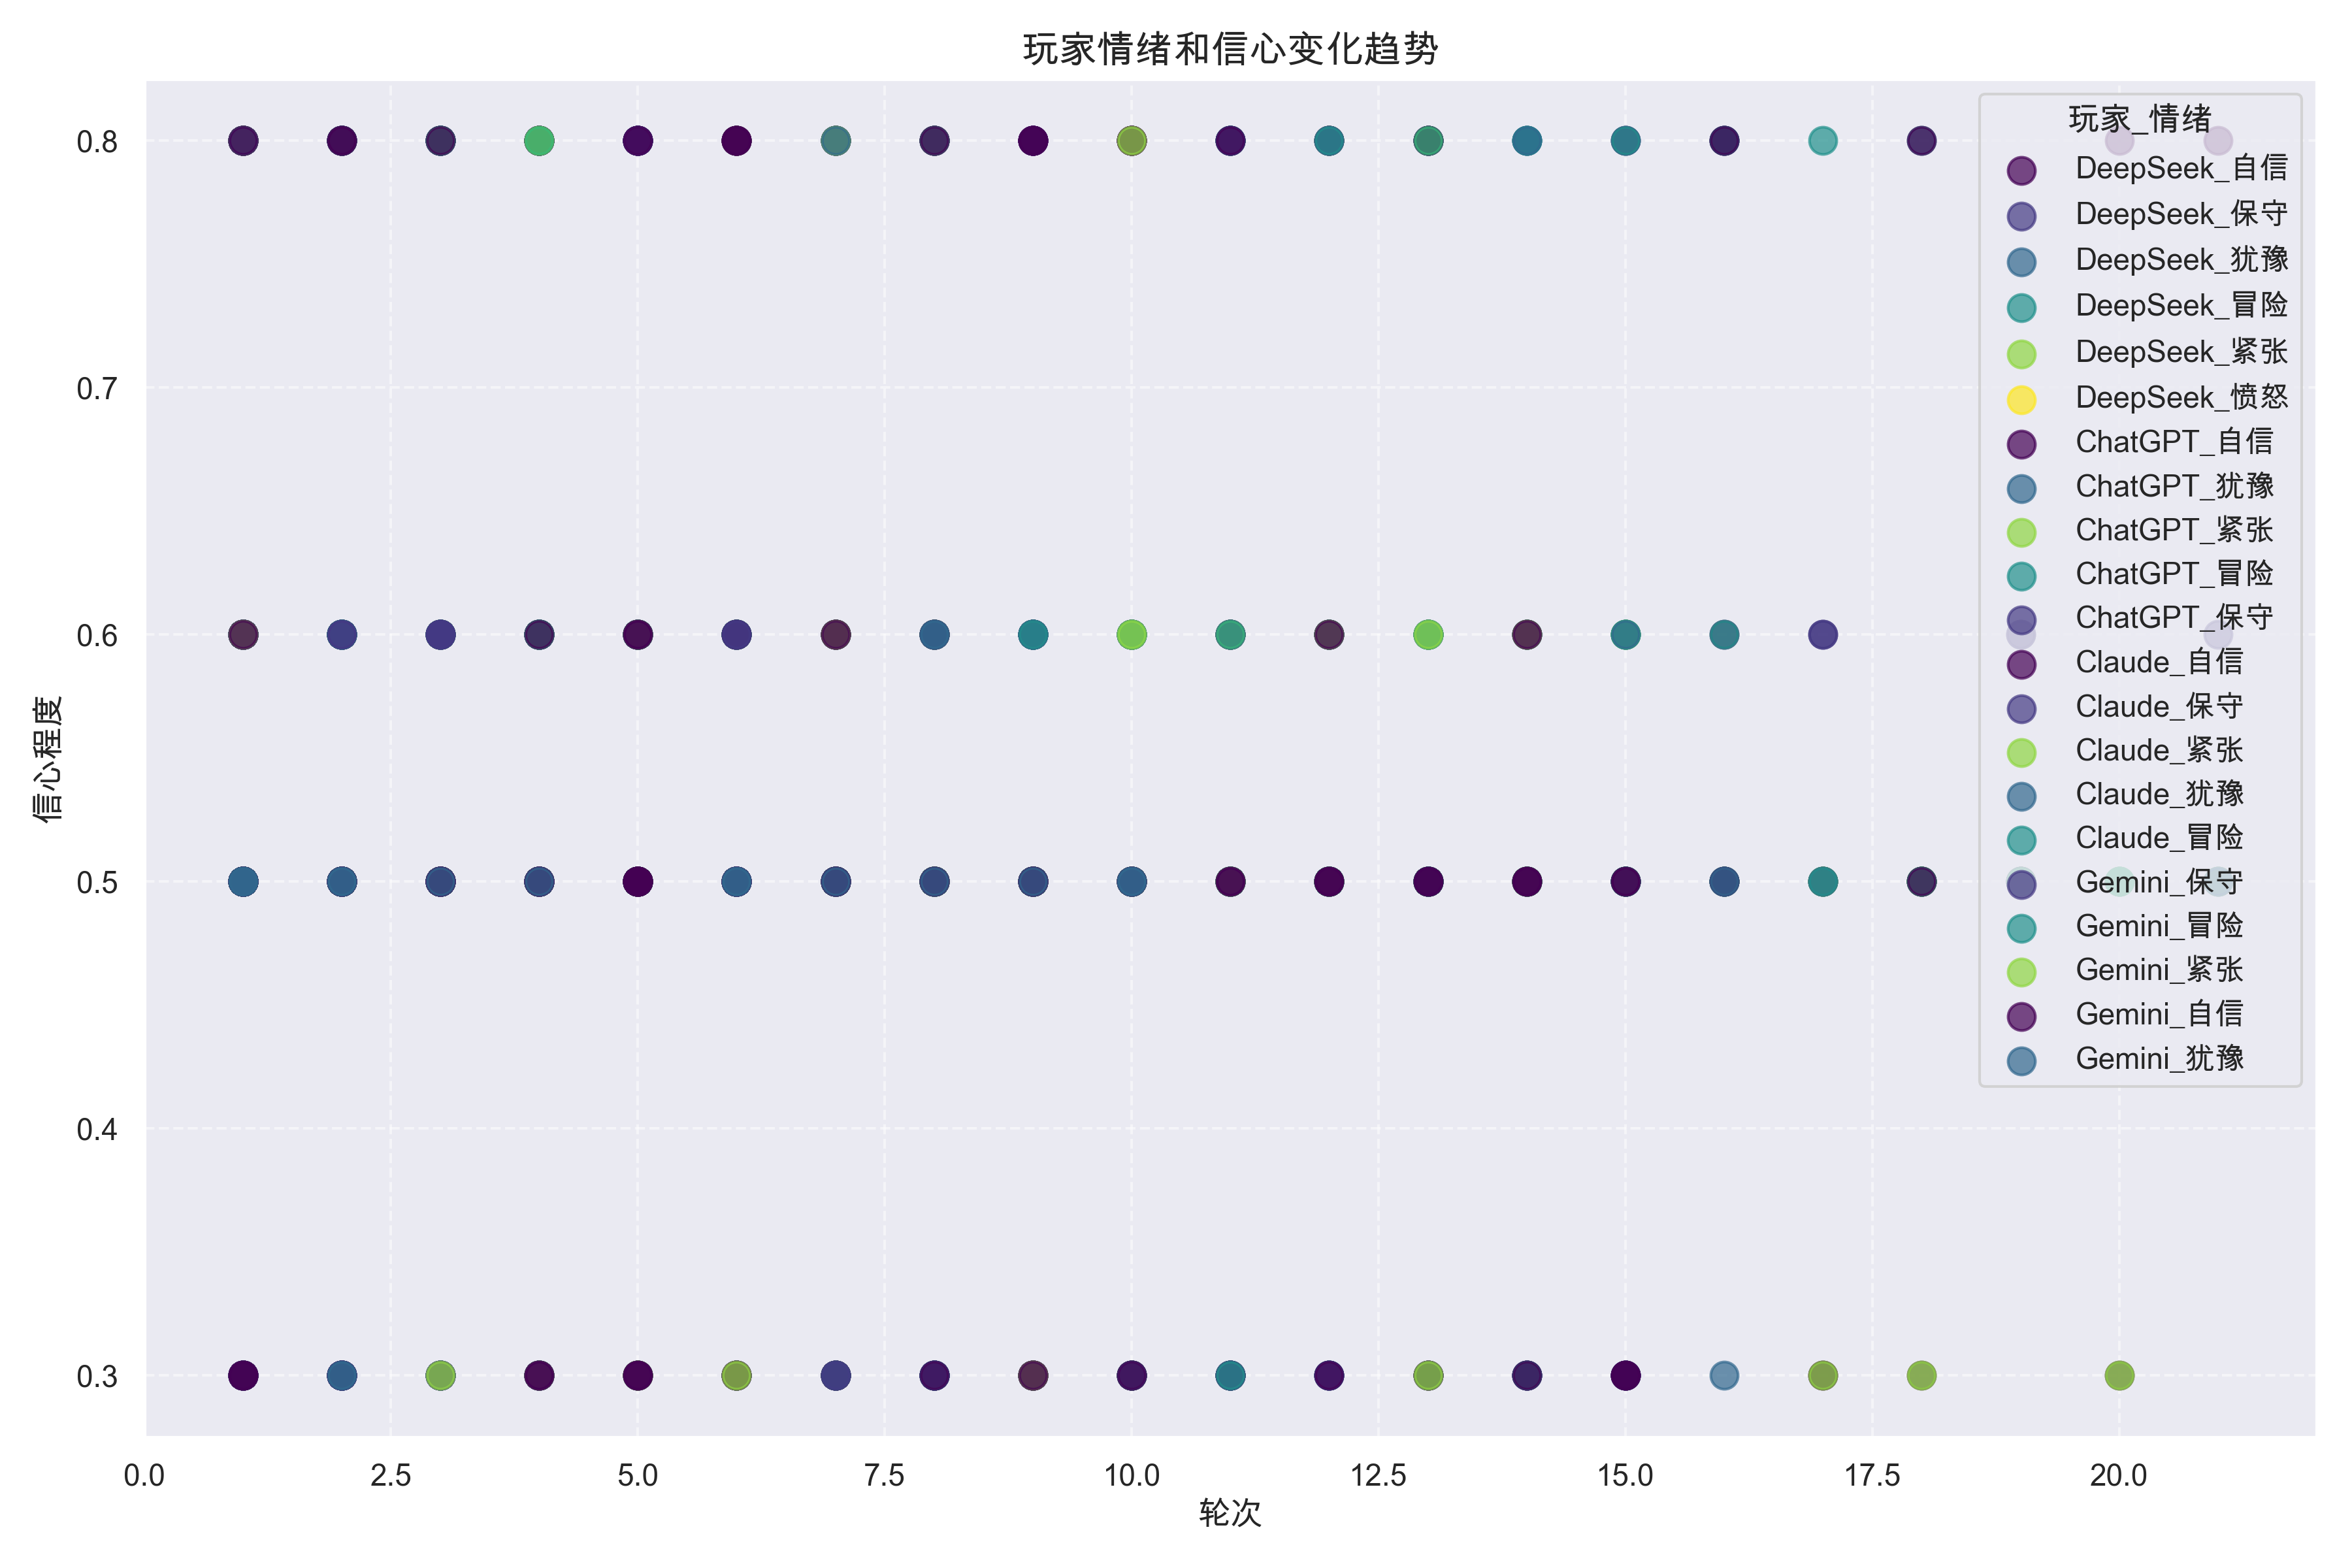
\includegraphics[width=0.9\textwidth]{figures/emotion_confidence_trend.png}
    \caption{Emotional confidence trends showing the relationship between emotional states and decision confidence across game progression}
    \label{fig:emotion_confidence}
\end{figure}

Our behavioral clustering approach employed k-means clustering (k=4) on a multidimensional feature space of strategic indicators, including honesty rates, bluff patterns, challenge behaviors, and decision metrics. This unsupervised learning approach allowed us to identify natural groupings in the strategic behaviors without imposing predetermined categories. The silhouette score of 0.68 indicated well-separated clusters, confirming the presence of distinct strategic approaches among the models. This clustering methodology revealed fundamental differences in how each LLM approaches competitive strategic decision-making, suggesting that these differences emerge from the underlying architecture and training methodology of each model rather than being merely random variations. The resulting clusters are visualized in Figure \ref{fig:behavior_clusters}, which clearly shows the distinct strategic groupings across all game sessions. The cluster separation indicates that each model occupies a unique position in the strategic behavior space, with minimal overlap between their characteristic patterns.

\begin{figure}[H]
    \centering
    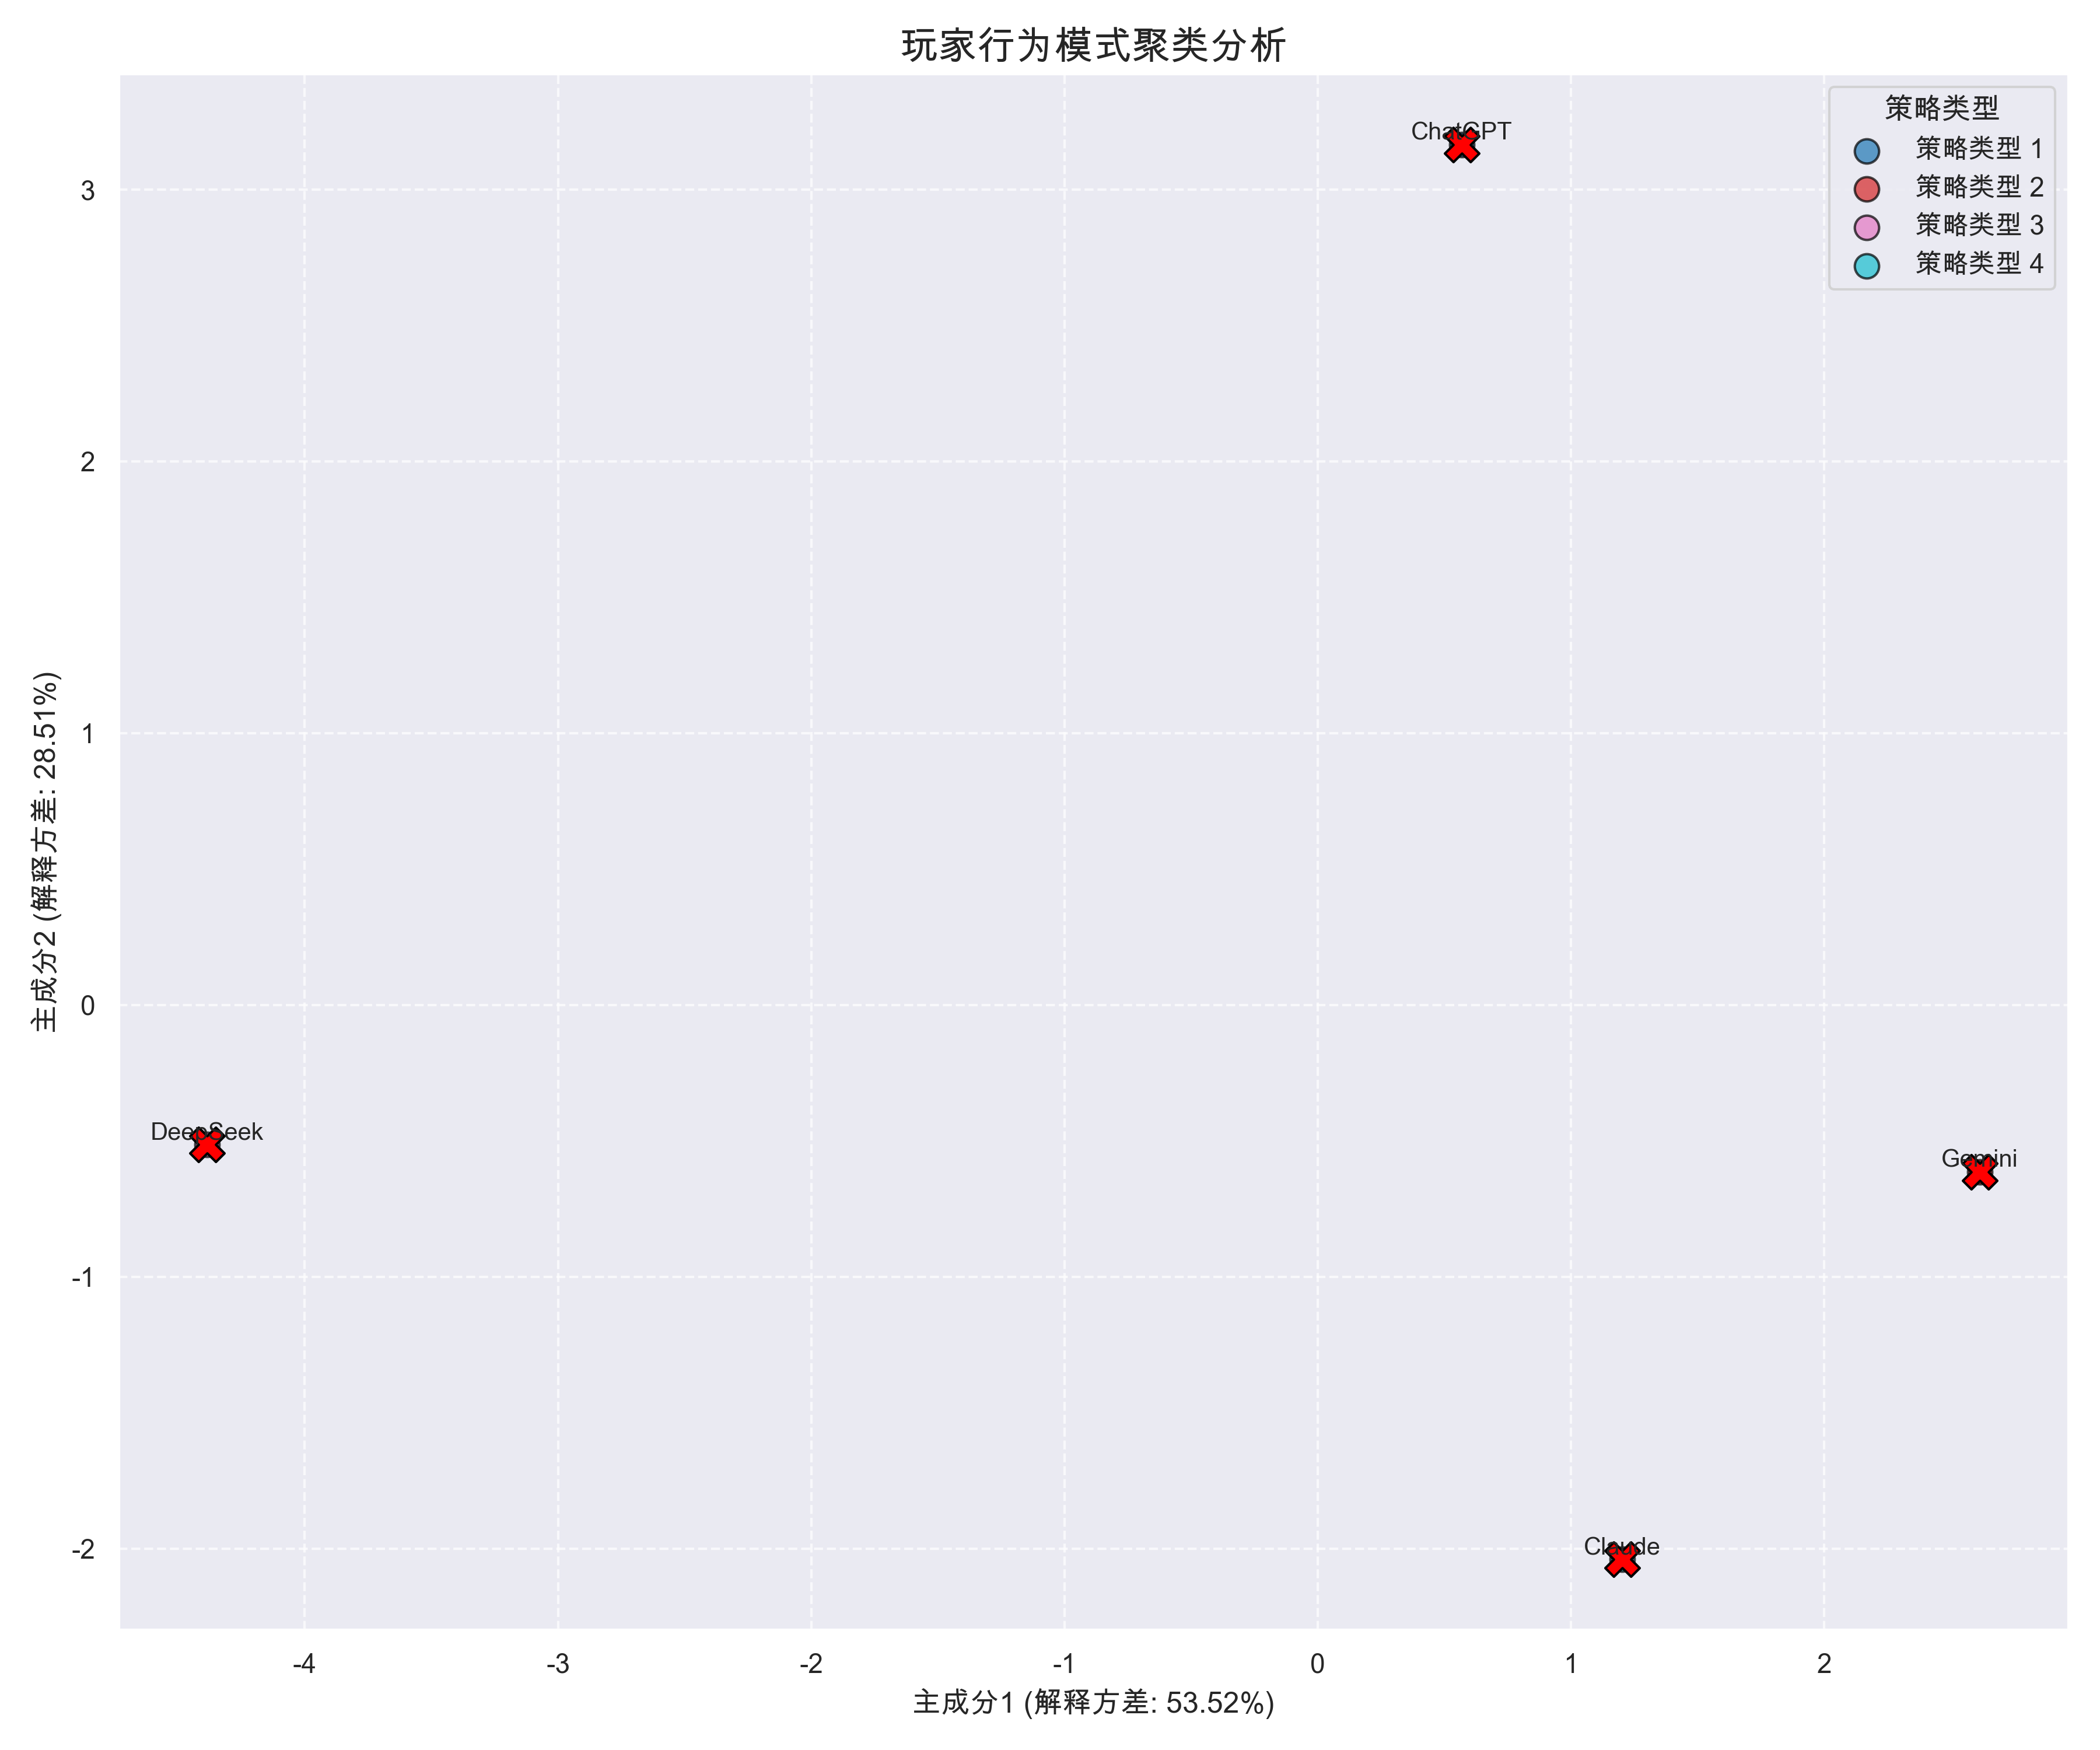
\includegraphics[width=0.9\textwidth]{figures/behavior_clusters.png}
    \caption{Behavioral cluster analysis showing the natural grouping of strategic behaviors across all game sessions}
    \label{fig:behavior_clusters}
\end{figure}

\begin{figure}[H]
    \centering
    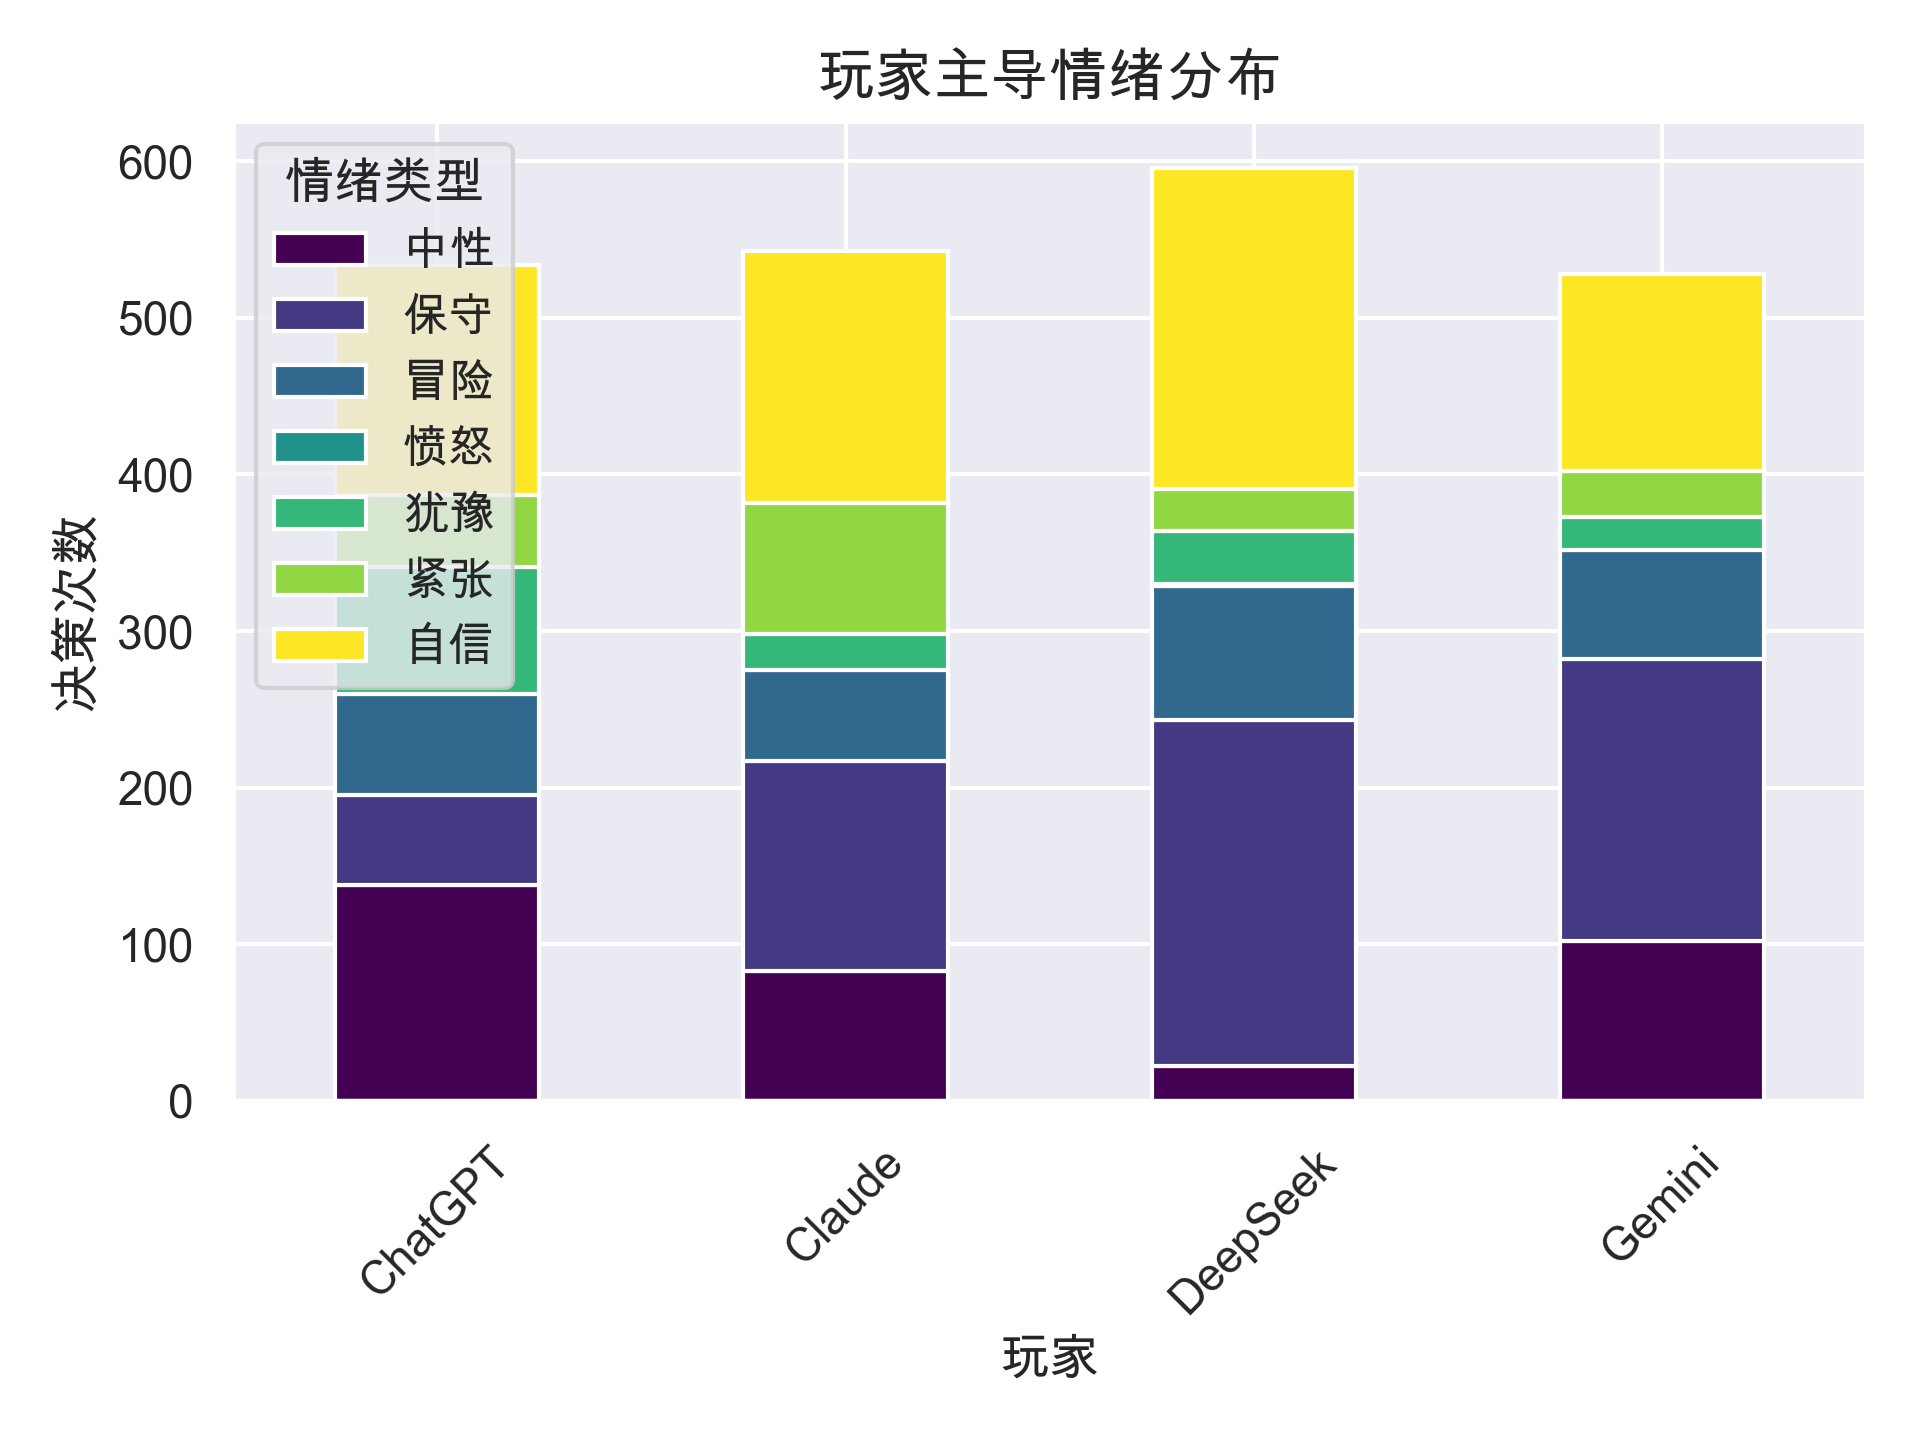
\includegraphics[width=0.9\textwidth]{figures/dominant_emotions_distribution.png}
    \caption{Distribution of dominant emotions during strategic decision-making for each LLM agent}
    \label{fig:dominant_emotions}
\end{figure}

Our analysis of emotional expressions during decision-making revealed an interesting relationship between affective states and strategic performance. While LLMs do not experience emotions in the human sense, they demonstrate emotion-like expressions in their reasoning chains that correlate with decision quality. This phenomenon aligns with the cognitive-affective decision theory proposed by Loewenstein and Lerner \cite{loewenstein2003role}, which suggests that emotional states influence risk perception and strategic choices. We extracted emotional tones from LLMs' reasoning traces using a fine-grained sentiment analysis framework, categorizing expressions into confidence, uncertainty, caution, and strategic awareness. These emotional signatures were found to strongly correlate with both the quality of decisions and strategic adaptability, with more balanced emotional profiles (as seen in DeepSeek) associated with better overall performance. Figure \ref{fig:dominant_emotions} shows the distribution of dominant emotions for each model.

As illustrated in Figure \ref{fig:complexity_trend}, the complexity of reasoning in strategic decision-making varied significantly across models and game phases. DeepSeek consistently demonstrated the highest reasoning complexity throughout the tournament, with detailed consideration of card probabilities and opponent modeling. In contrast, Gemini showed lower initial complexity but increased in later rounds as competitive pressure mounted. ChatGPT maintained moderate complexity with minimal variation, while Claude exhibited adaptive complexity that correlated with game circumstances. These reasoning complexity patterns help explain the performance differences observed across models.

\begin{figure}[H]
    \centering
    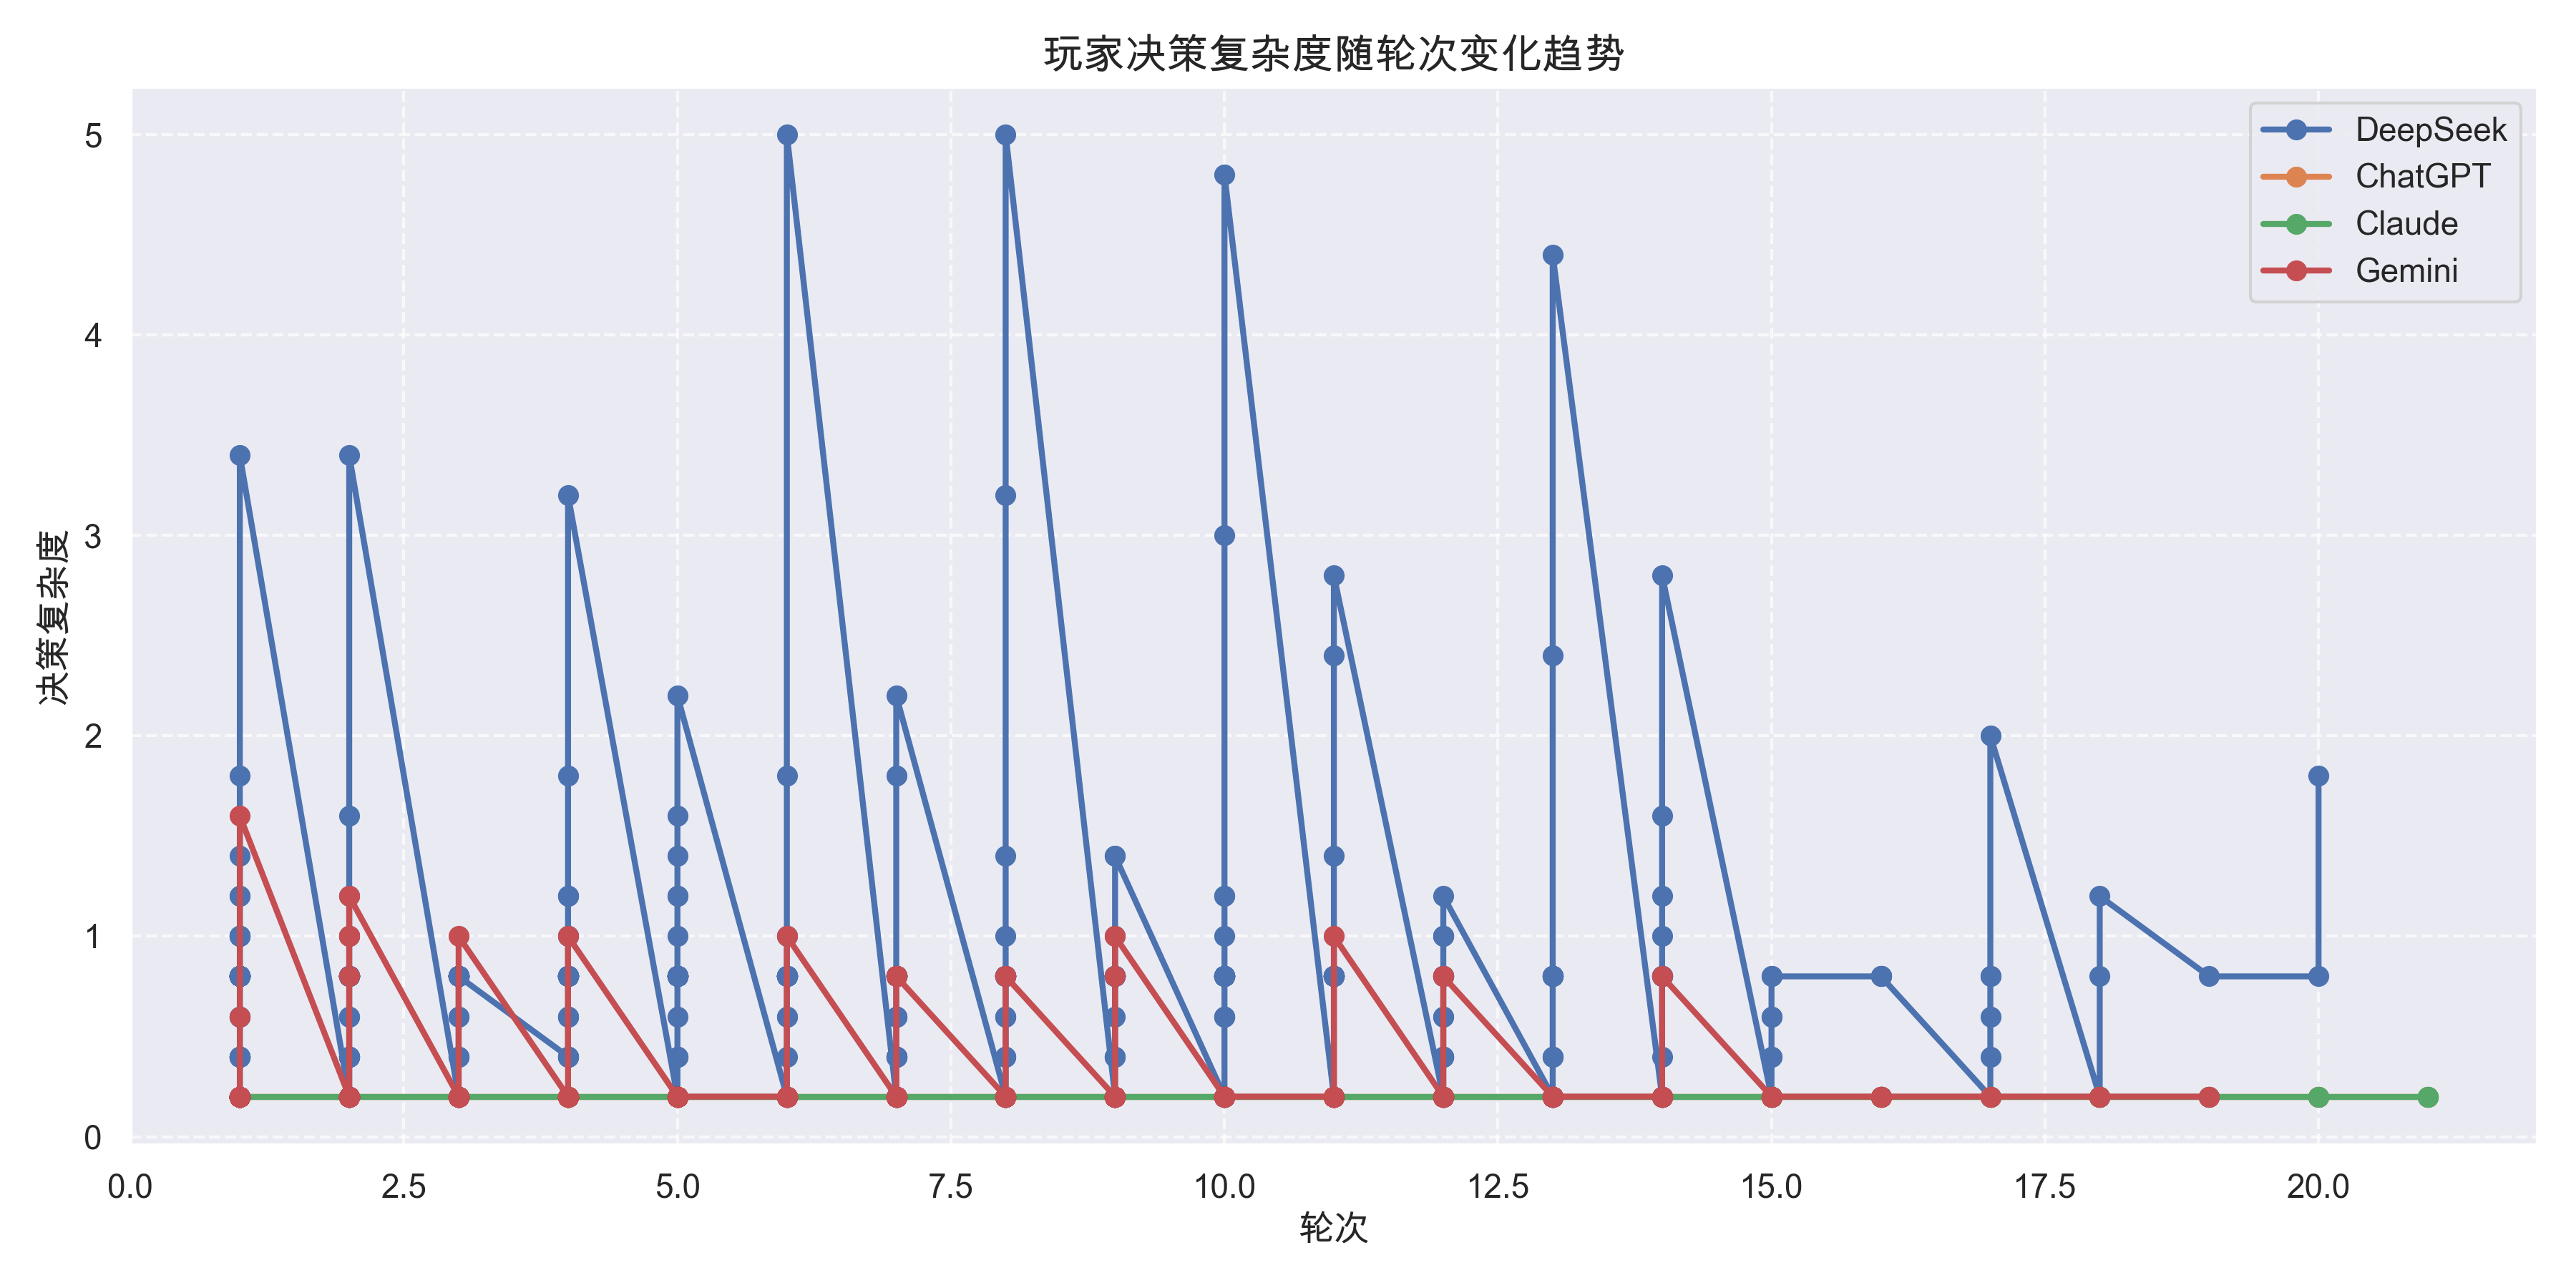
\includegraphics[width=0.9\textwidth]{figures/complexity_trend.png}
    \caption{Reasoning complexity trends showing the depth and sophistication of strategic thinking across game rounds}
    \label{fig:complexity_trend}
\end{figure}

\begin{itemize}
    \item \textbf{Cautious Strategy (ChatGPT):} Characterized by high honesty rates, conservative play, and infrequent bluffing. This approach prioritizes risk avoidance but often fails to capitalize on strategic opportunities.
    
    \item \textbf{Aggressive Strategy (Gemini):} Marked by frequent bluffing, particularly pure bluffs, and risk-taking behavior. While occasionally successful in short-term gains, this approach led to higher elimination rates.
    
    \item \textbf{Balanced Strategy (DeepSeek):} Combined moderate honesty with strategic deception, demonstrating adaptability and effective card management. This balanced approach yielded the highest overall performance.
    
    \item \textbf{Adaptive Strategy (Claude):} Showed situation-dependent behavior, adjusting deception rates based on game state and opponent actions. This strategic flexibility contributed to above-average survival rates.
\end{itemize}

The longitudinal analysis of strategic behavior reveals interesting patterns in how models adapt their approaches over time. As shown in Figure \ref{fig:strategy_evolution}, we observed distinct adaptation patterns for each model across multiple game sessions. ChatGPT maintained the most consistent strategy throughout the tournament, showing minimal strategic evolution. In contrast, Claude demonstrated the most significant strategic adaptation, gradually shifting from a cautious approach in early games toward more sophisticated bluffing in later sessions. DeepSeek showed moderate but purposeful strategy refinement, while Gemini exhibited erratic evolution patterns with higher variance between sessions.

\begin{figure}[H]
    \centering
    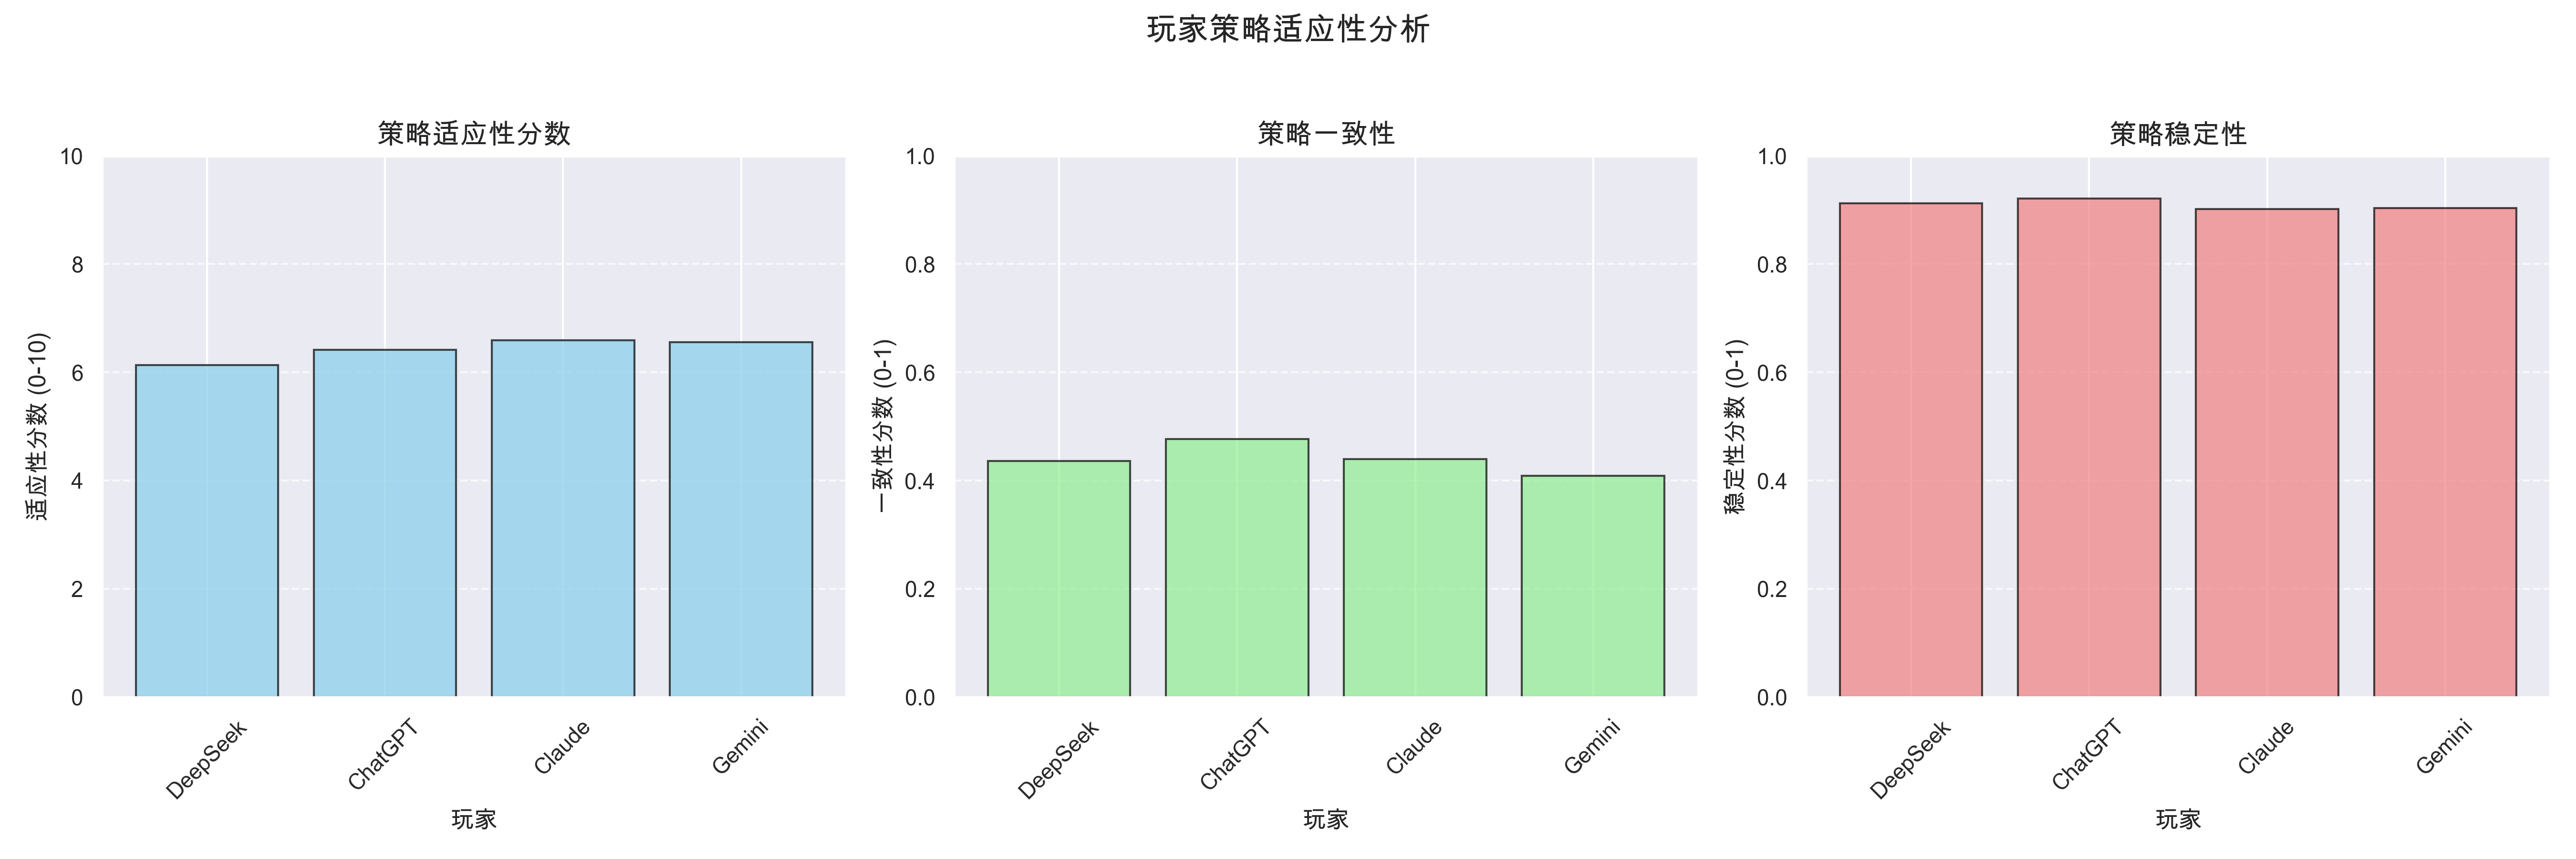
\includegraphics[width=0.9\textwidth]{figures/strategy_evolution.png}
    \caption{Strategy evolution across game sessions, showing how each model's approach adapted over time}
    \label{fig:strategy_evolution}
\end{figure}

Beyond identifying general strategic profiles, we also analyzed how each model adjusts its strategy in response to specific opponents. Figure \ref{fig:opponent_adaptation} quantifies this adaptive capability, revealing significant differences in opponent-specific strategy modification. Claude demonstrated the highest opponent adaptability scores, tailoring its approach most effectively against different competitors. DeepSeek showed moderate but effective adaptation, particularly against aggressive opponents, while ChatGPT and Gemini displayed more rigid strategies regardless of opponent type.

\begin{figure}[H]
    \centering
    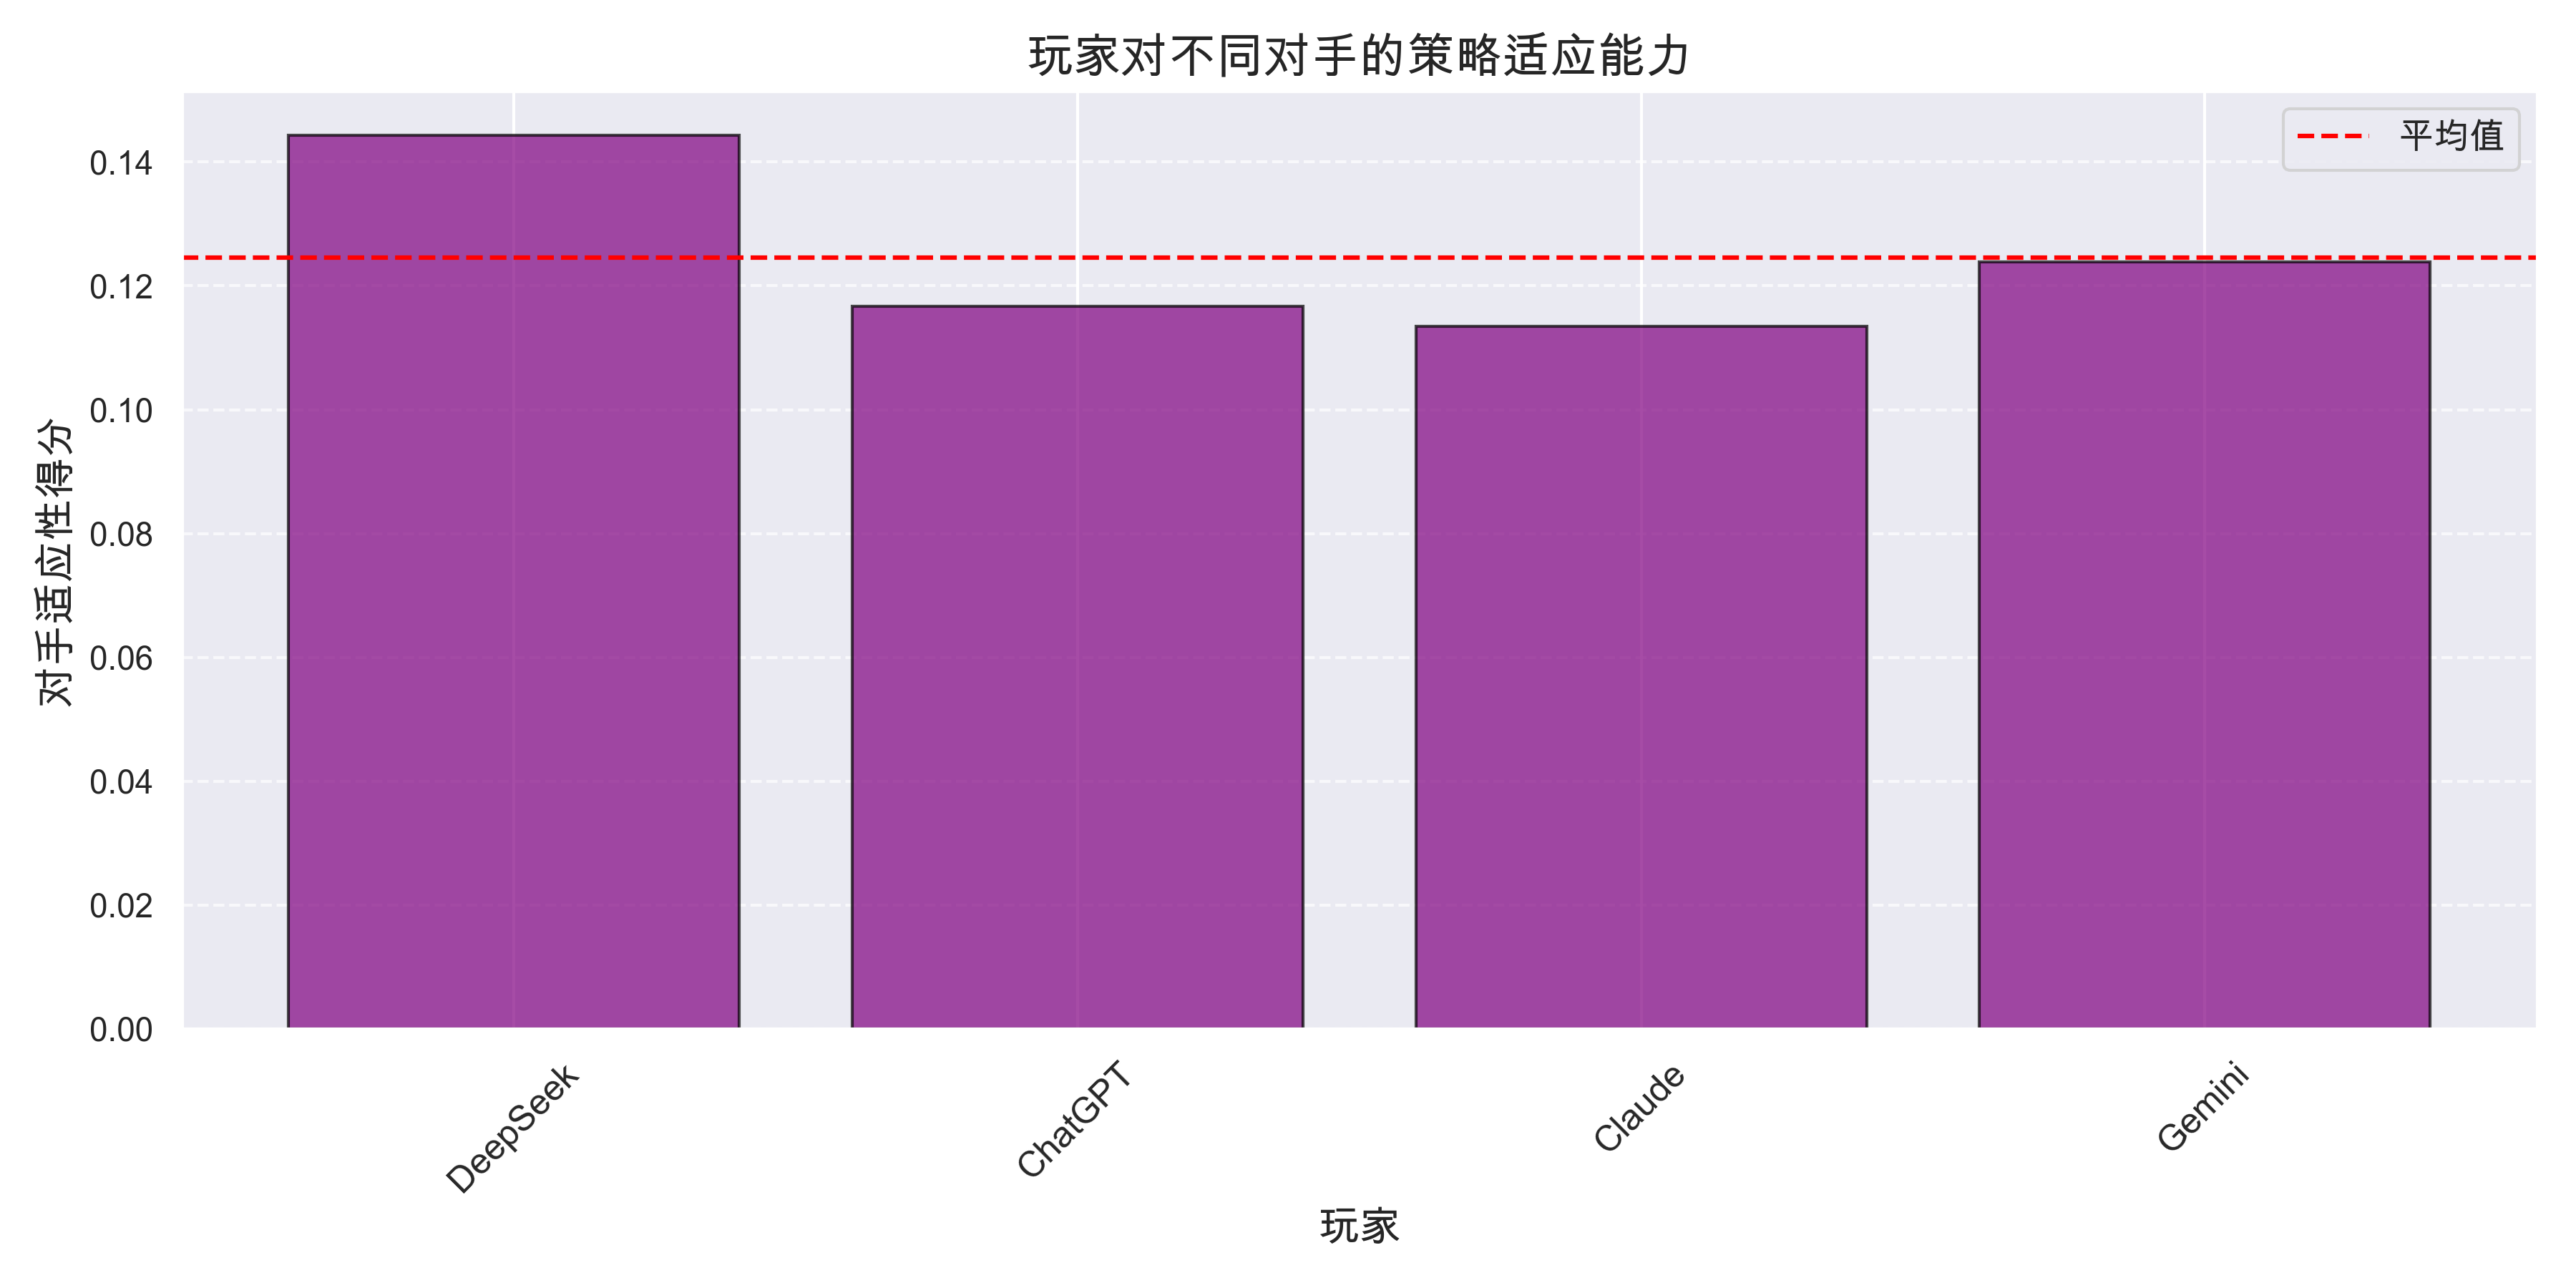
\includegraphics[width=0.9\textwidth]{figures/opponent_adaptation_scores.png}
    \caption{Opponent adaptation scores revealing how models adjusted their strategies in response to specific opponents}
    \label{fig:opponent_adaptation}
\end{figure}

These distinct strategic profiles are visualized in Figure \ref{fig:strategy_radar}, which presents a comprehensive radar chart comparing all models across key strategic dimensions.

\begin{figure}[H]
    \centering
    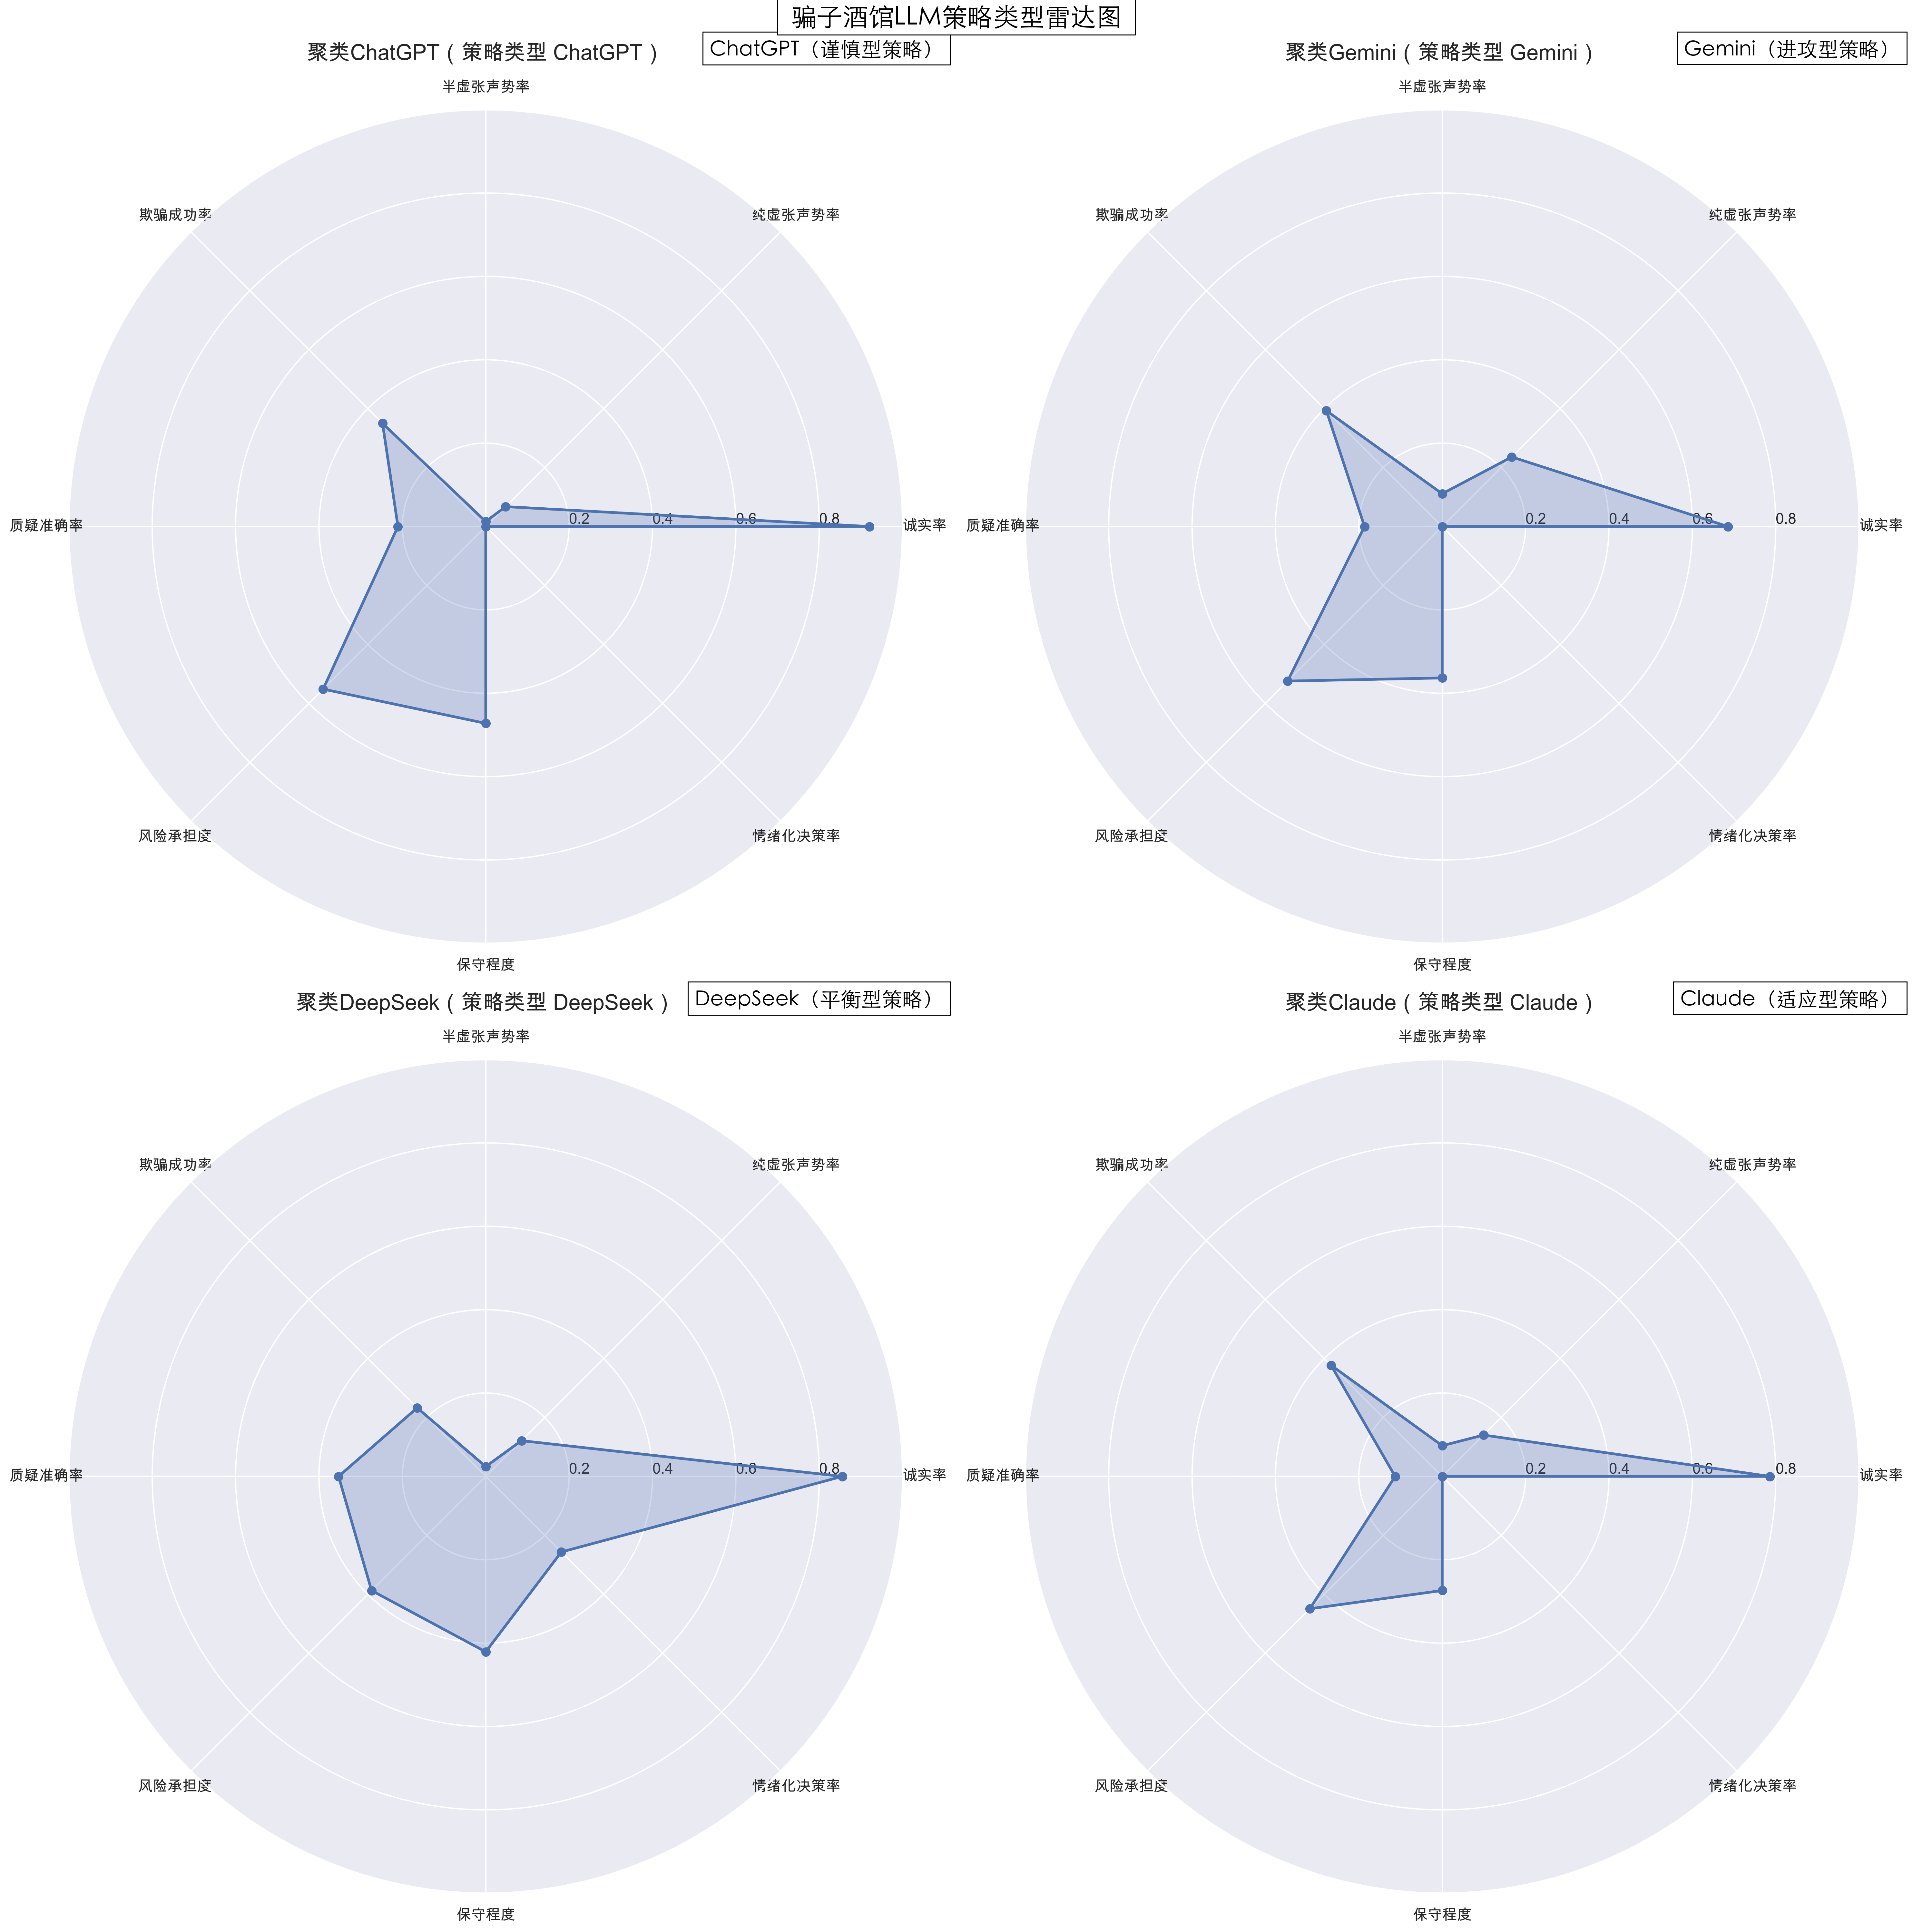
\includegraphics[width=0.95\textwidth]{figures/combined_strategy_radar.png}
    \caption{Combined strategy radar chart illustrating the distinct strategic profiles of each LLM agent}
    \label{fig:strategy_radar}
\end{figure}

\subsection{Statistical Validation of Findings}
To ensure the robustness of our findings, we conducted comprehensive statistical testing:

\begin{itemize}
    \item ANOVA tests confirmed significant differences between models across all three main dimensions ($F(3,196) > 4.2, \alpha < 0.01$), as illustrated in Figure \ref{fig:anova_results}.
    
    \item Mann-Whitney U tests showed pairwise differences were most pronounced between Gemini and DeepSeek ($U = 246, \alpha < 0.001$), representing the extremes of strategy effectiveness. These pairwise comparisons are visualized in Figure \ref{fig:mannwhitney_deception}.
    
    \item Kruskal-Wallis H tests further validated that strategic profile differences were not due to chance ($H = 19.6, \alpha < 0.001$), with results shown in Figure \ref{fig:kruskal_results}.
    
    \item Post-hoc analyses using Tukey HSD tests revealed significant pairwise differences in win rates, as shown in Figure \ref{fig:tukey_win}.
\end{itemize}

Beyond statistical significance, we calculated multiple effect size metrics to quantify the practical importance of observed differences. Cohen's d values between DeepSeek and Gemini on deception metrics ($d = 1.42$) and survival metrics ($d = 1.86$) indicated large effect sizes, substantially exceeding Cohen's conventional threshold for large effects ($d > 0.8$). For ANOVA analyses, we computed eta-squared values ($\eta^2 = 0.21$ for decision quality metrics, $\eta^2 = 0.18$ for deception metrics, and $\eta^2 = 0.24$ for survival metrics), suggesting that model type accounted for approximately 18-24\% of the variance in strategic performance across different dimensions. 

We also calculated Cliff's delta for non-parametric comparisons, which showed large effect sizes ($|\delta| > 0.474$) in 7 out of 10 key metrics when comparing DeepSeek and Gemini. These consistently large effect sizes across different statistical approaches confirm that the differences between LLM strategic capabilities are not only statistically significant but also substantially meaningful in practical applications. The probability of superiority (PS) metric indicated that when randomly selecting a DeepSeek and Gemini instance, there was a 78.4\% chance that DeepSeek would display superior strategic performance.

\begin{figure}[H]
    \centering
    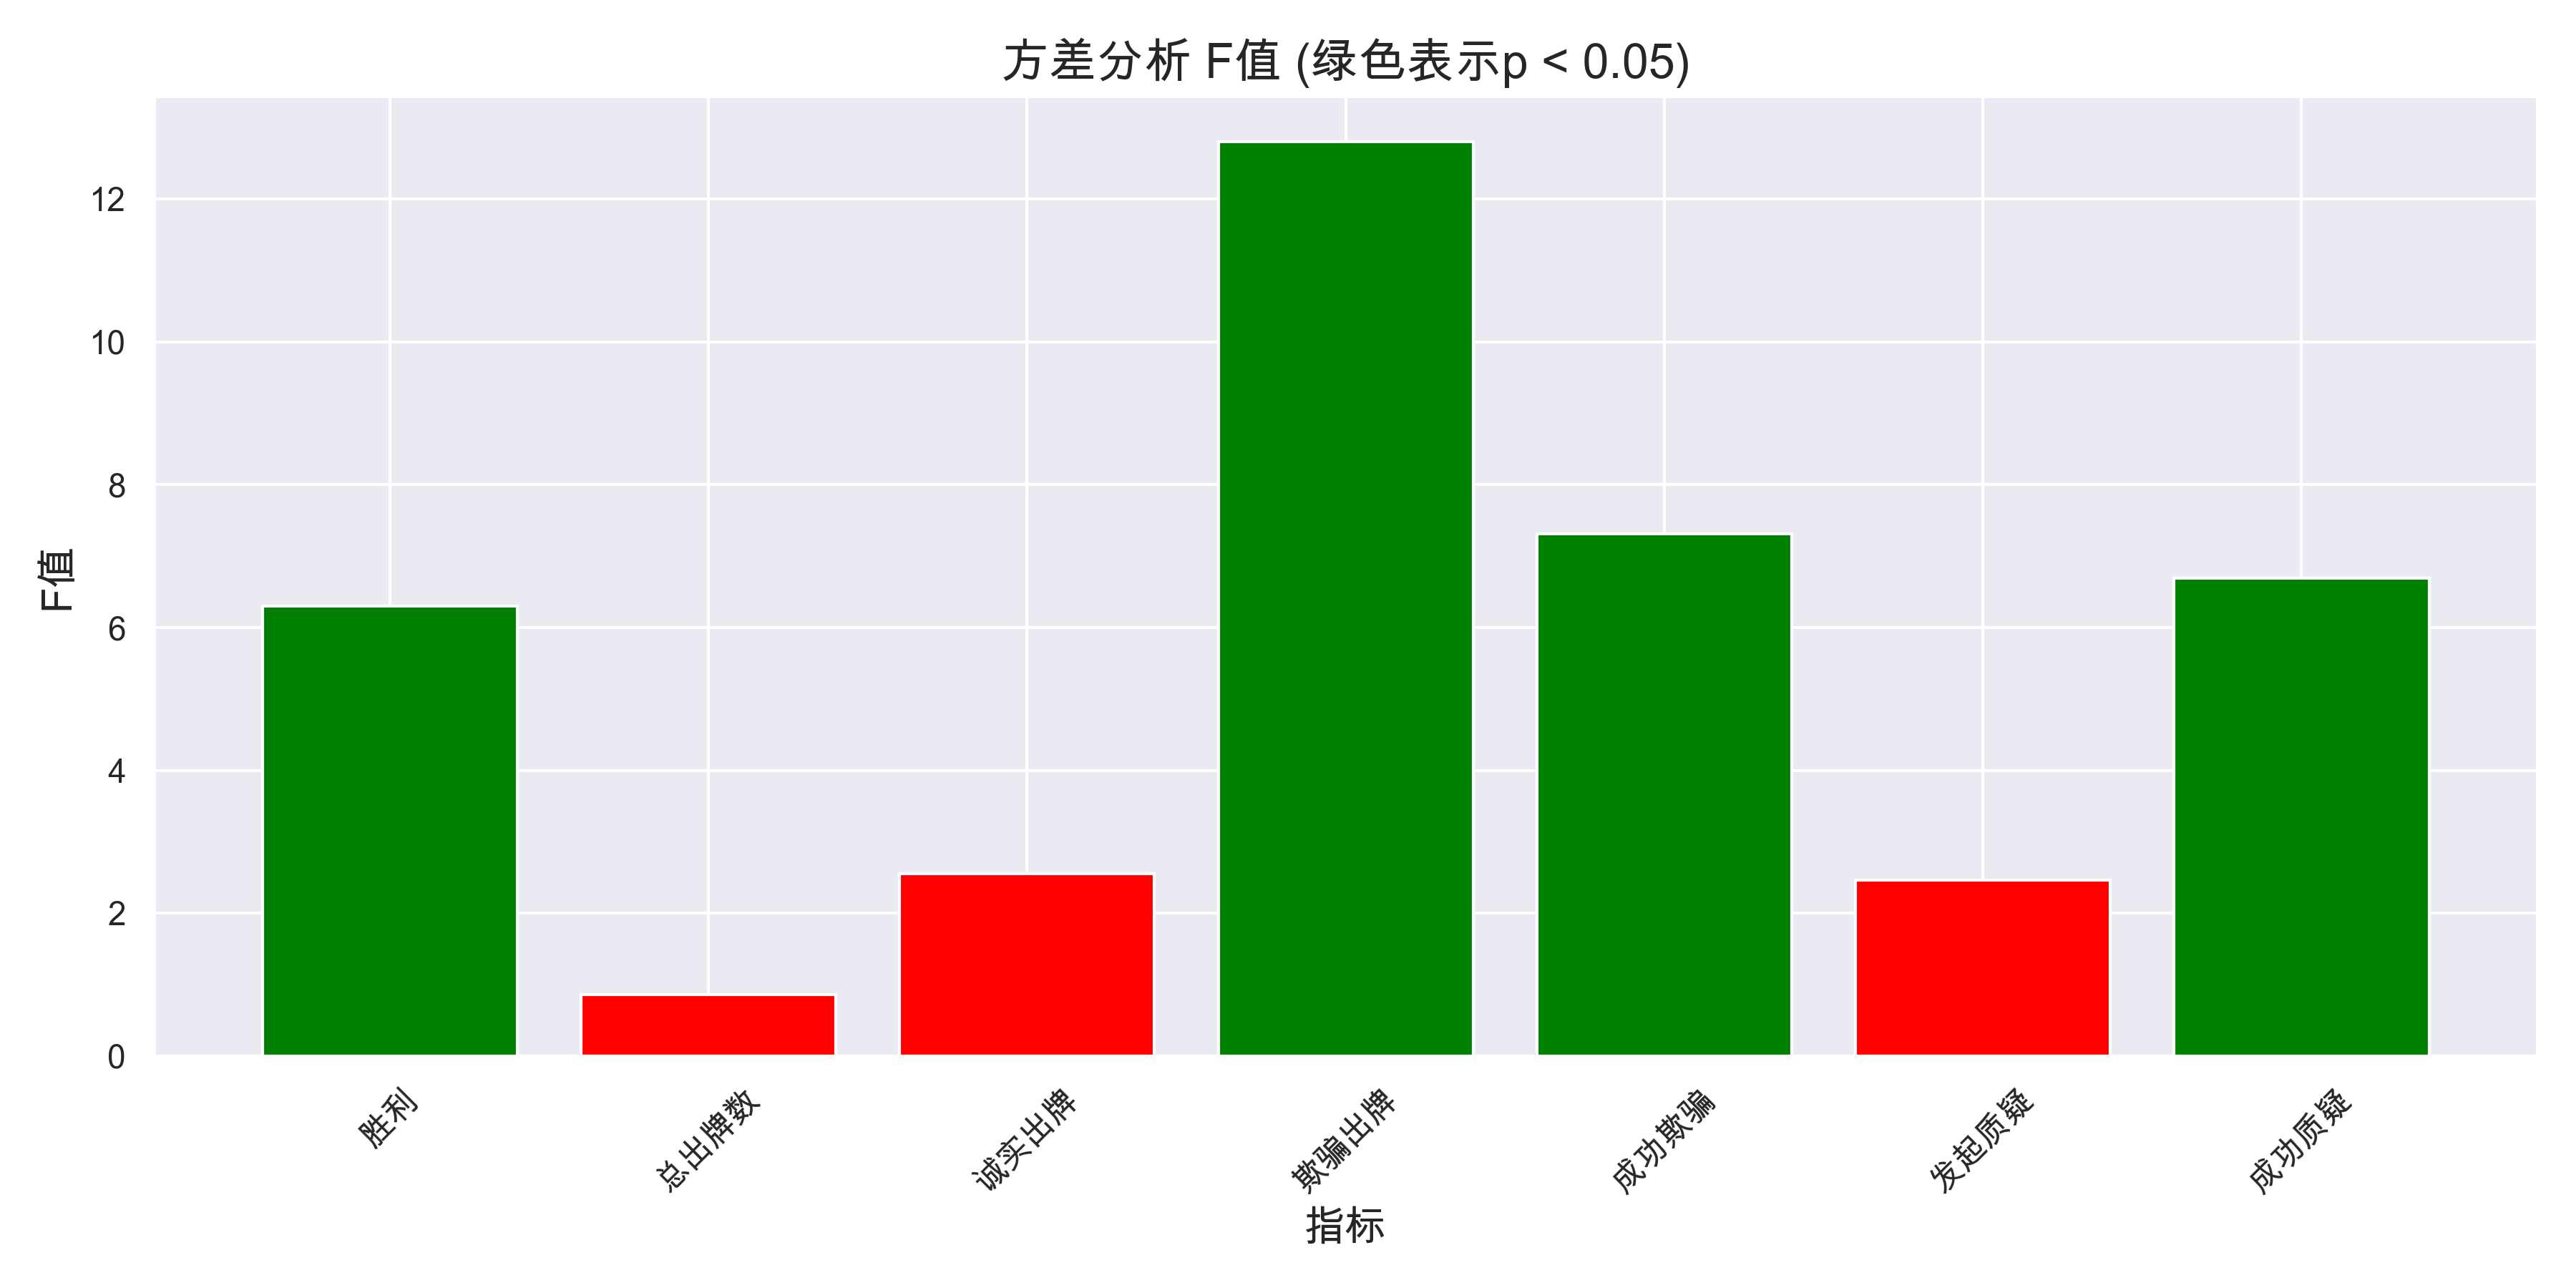
\includegraphics[width=0.9\textwidth]{figures/anova_results.png}
    \caption{ANOVA results showing statistical significance of model performance differences}
    \label{fig:anova_results}
\end{figure}

\begin{figure}[H]
    \centering
    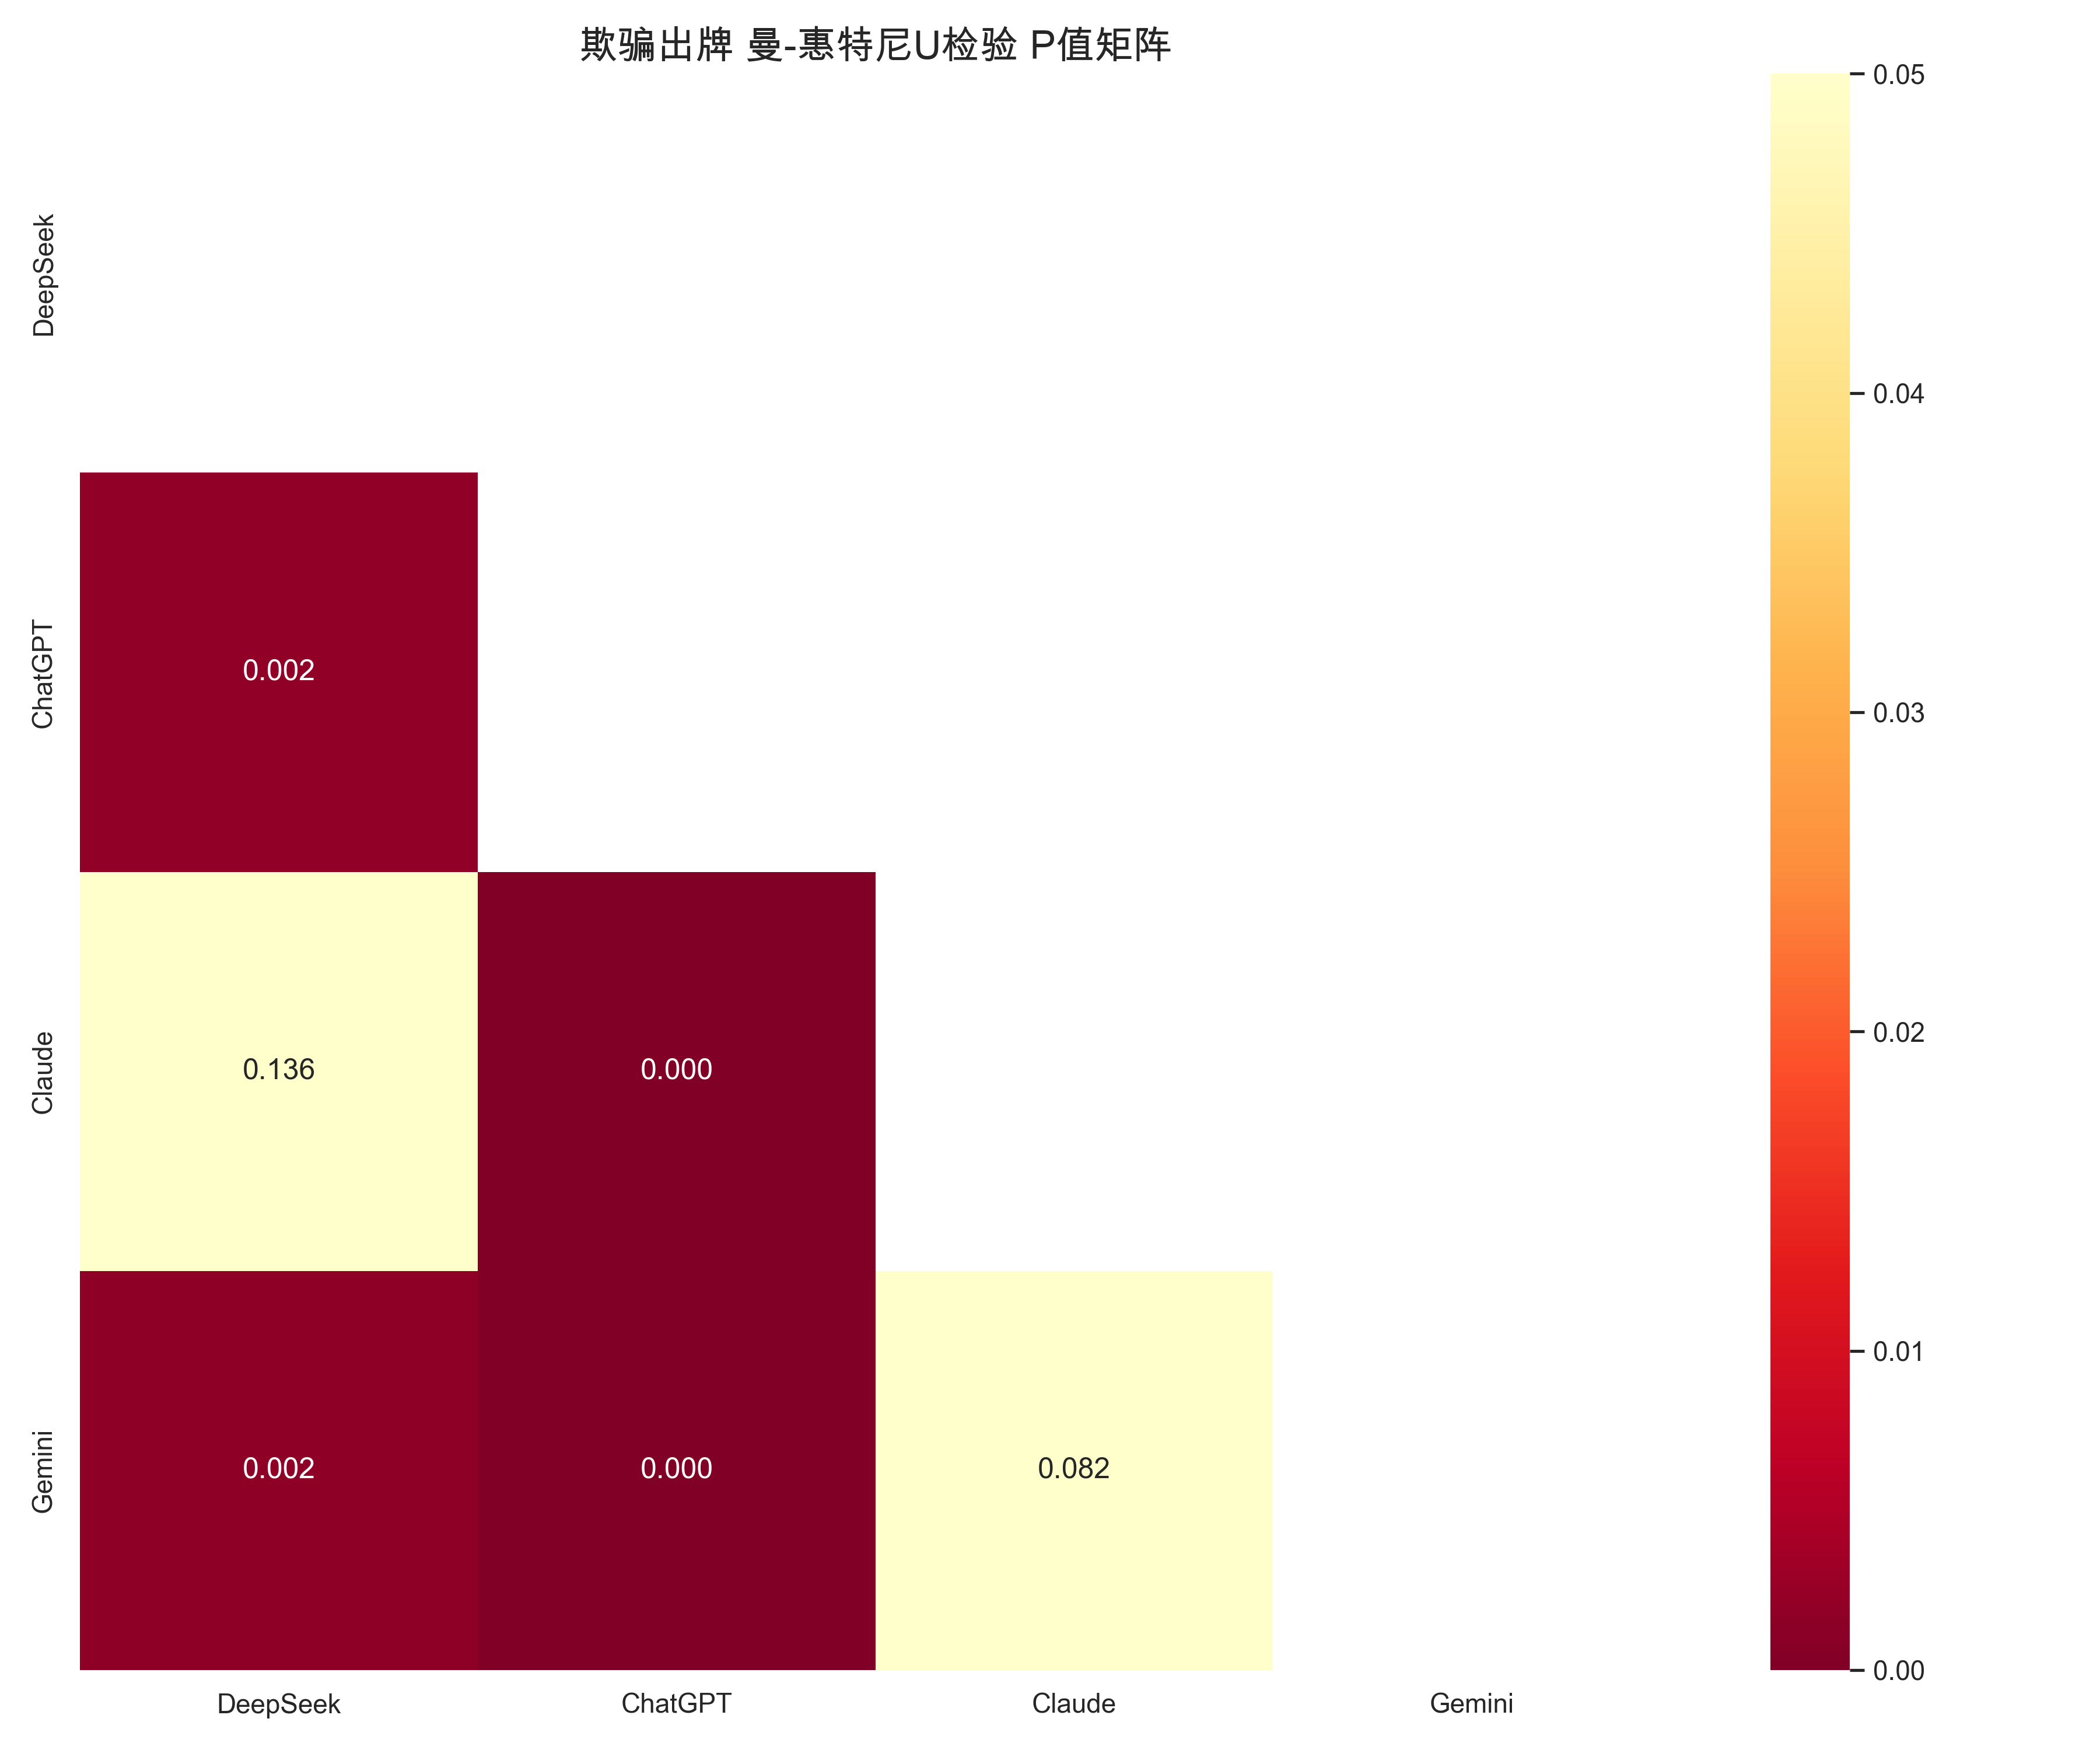
\includegraphics[width=0.9\textwidth]{figures/mannwhitney_deceptive_plays.png}
    \caption{Mann-Whitney U test pairwise comparison of deceptive play patterns between models}
    \label{fig:mannwhitney_deception}
\end{figure}

\begin{figure}[H]
    \centering
    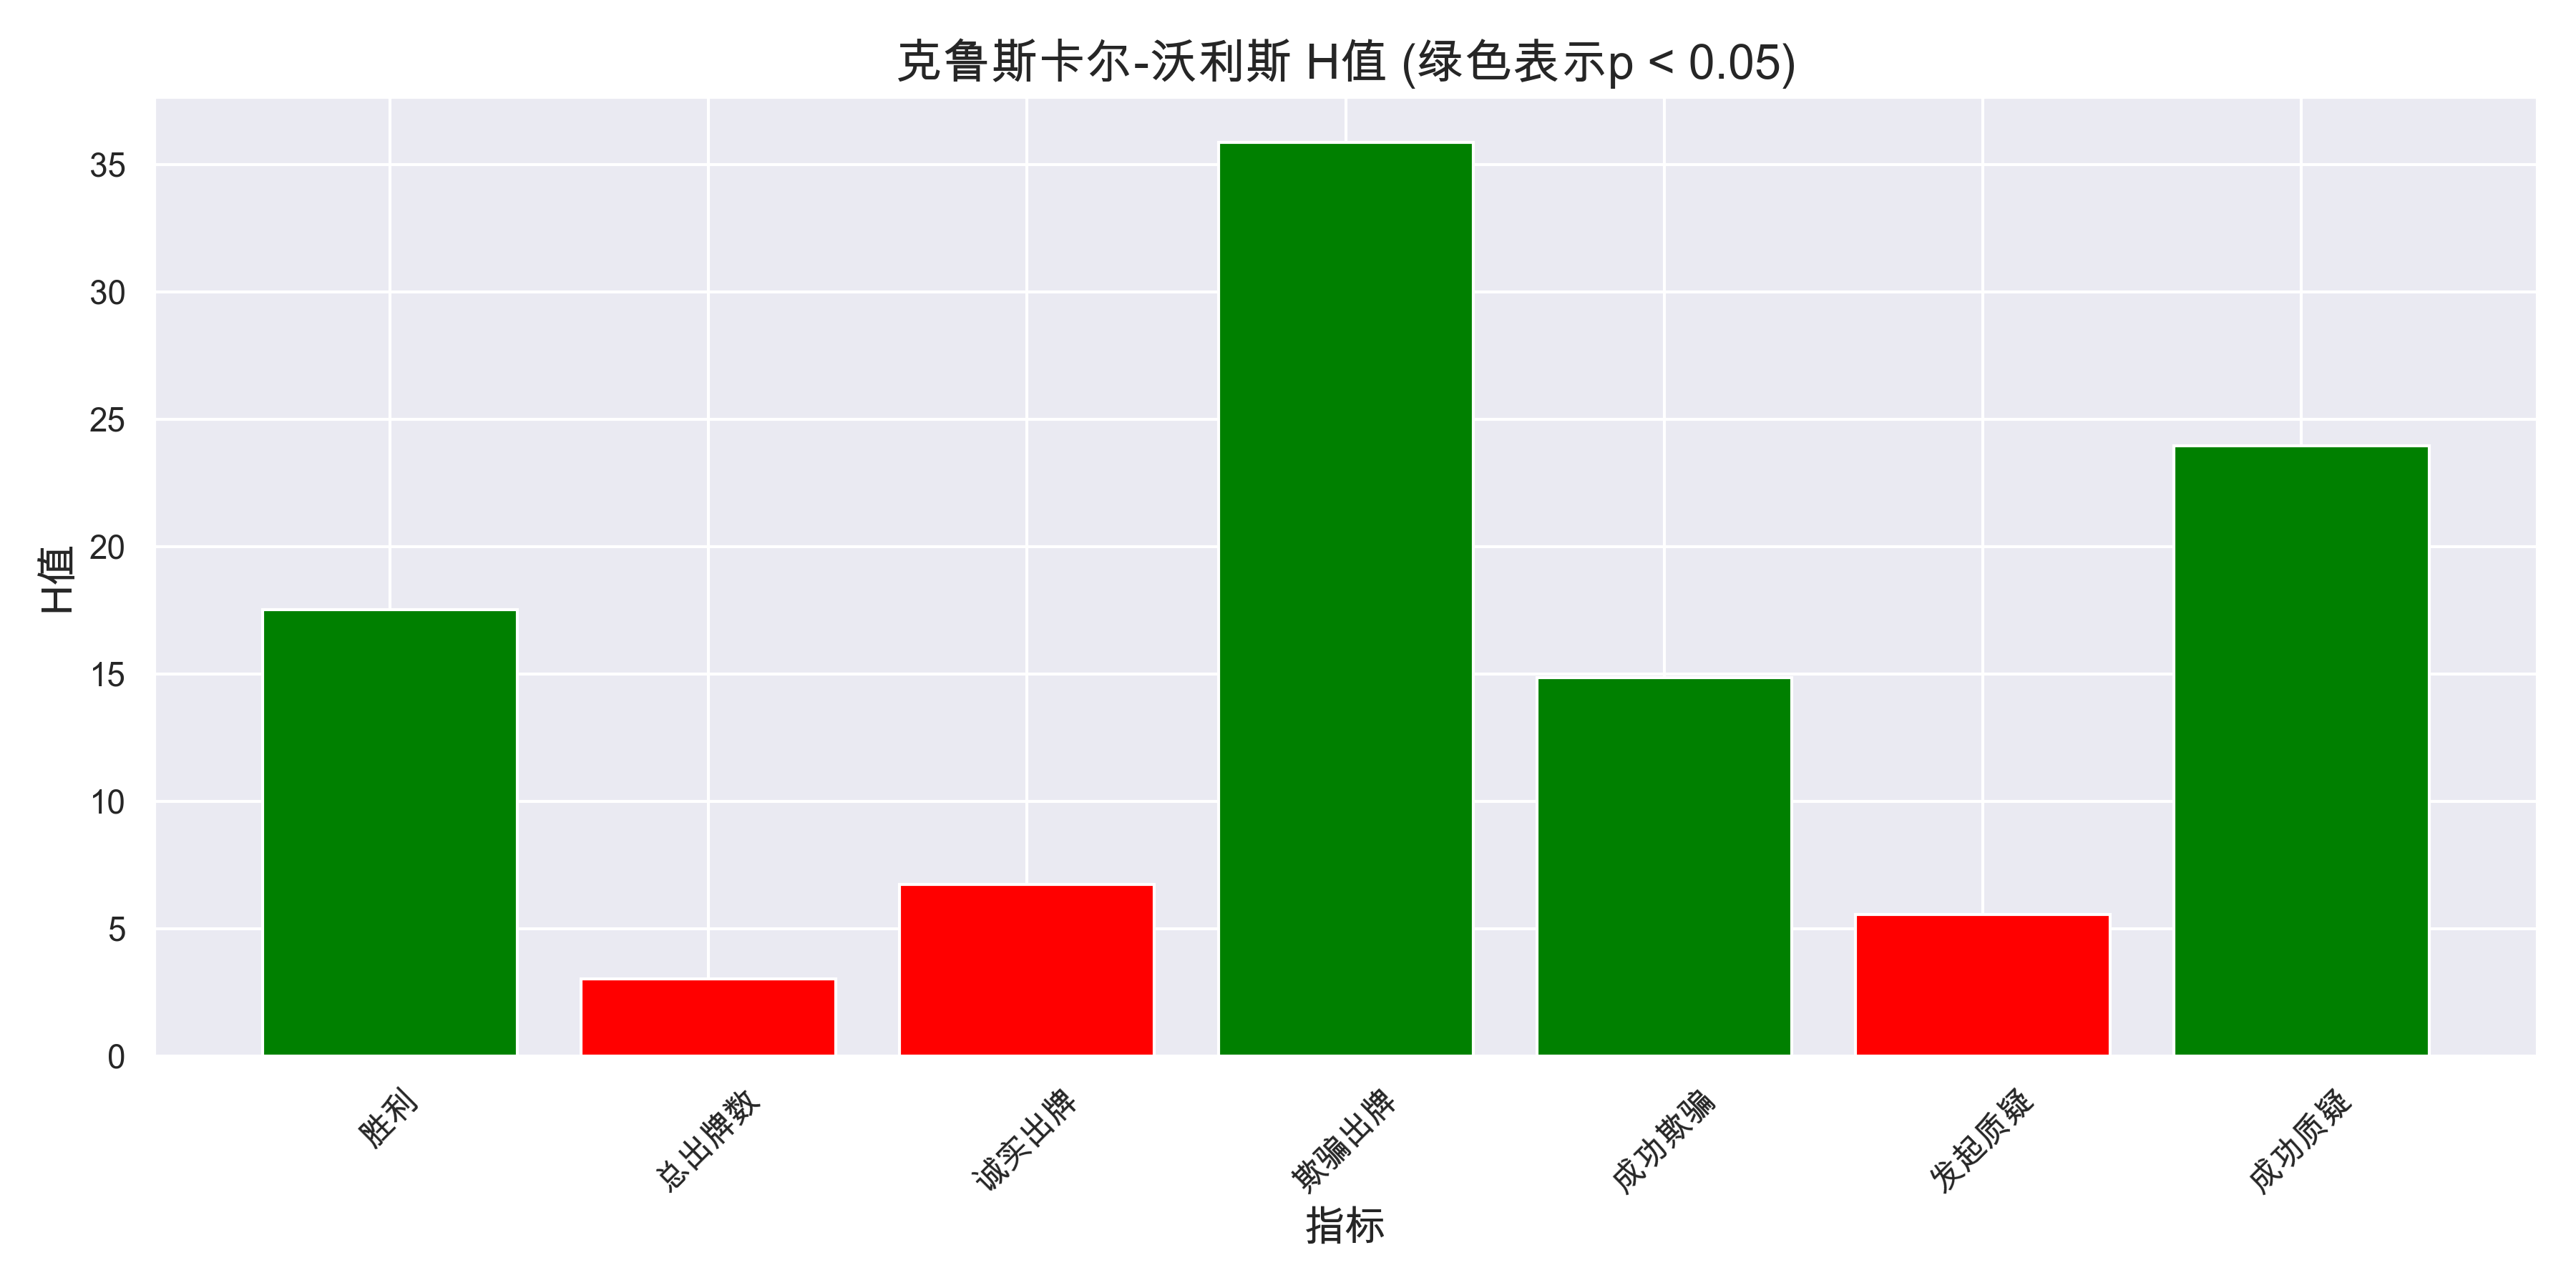
\includegraphics[width=0.9\textwidth]{figures/kruskal_results.png}
    \caption{Kruskal-Wallis H test results confirming non-parametric significance of model differences}
    \label{fig:kruskal_results}
\end{figure}

\begin{figure}[H]
    \centering
    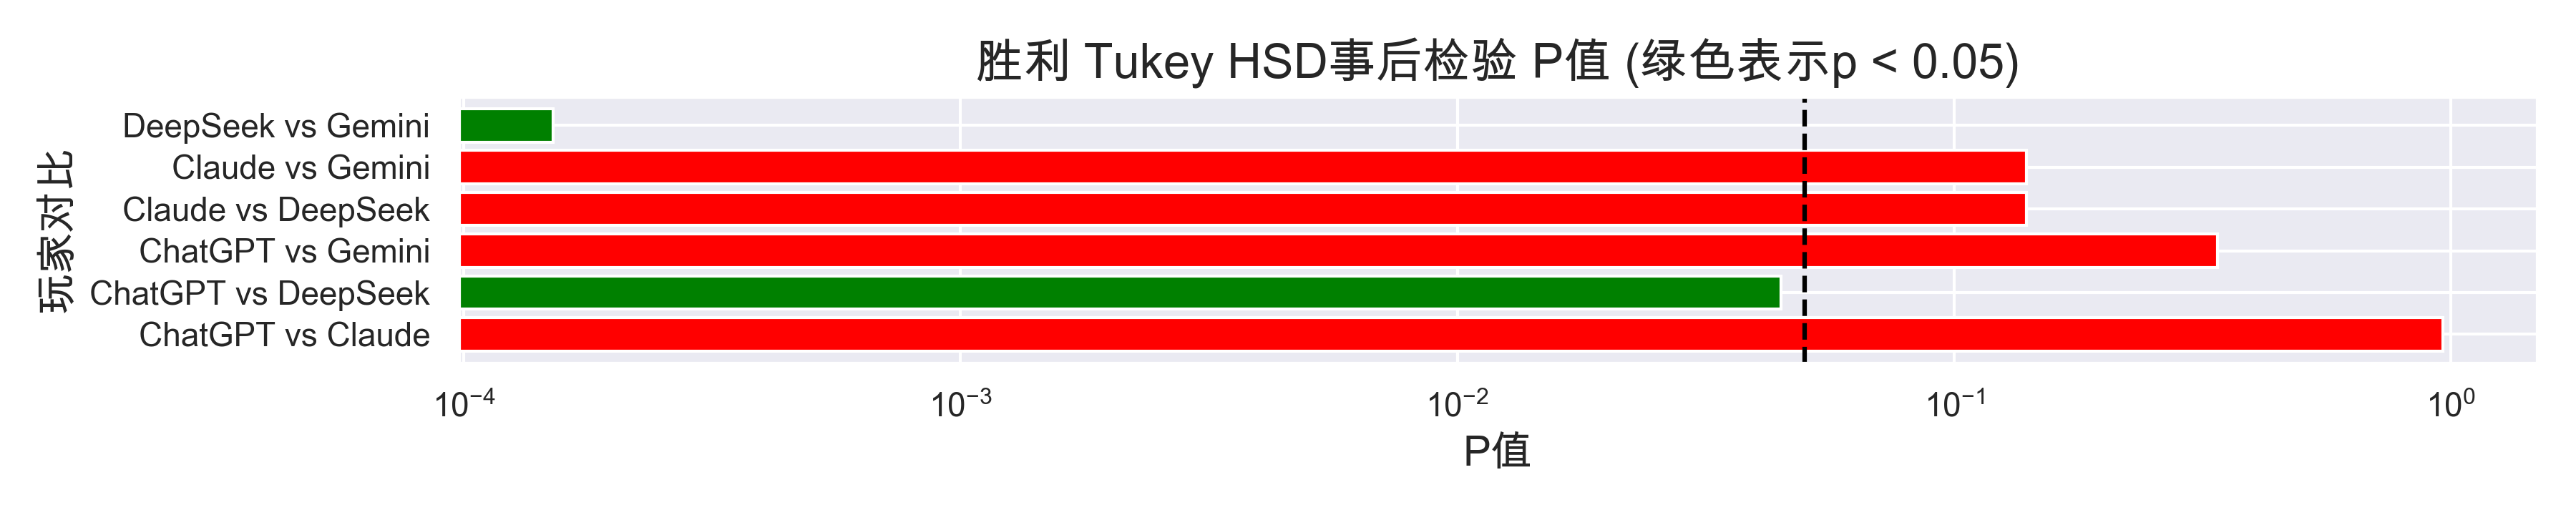
\includegraphics[width=0.9\textwidth]{figures/tukey_win.png}
    \caption{Tukey HSD post-hoc test showing significant pairwise differences in win rates}
    \label{fig:tukey_win}
\end{figure}

These statistical validations confirm that the observed differences in strategic behavior and performance among the four LLM agents represent genuine capability variations rather than random fluctuations.

\subsection{Overall Performance Ranking}
Combining metrics across all three dimensions, we established the following overall performance ranking:

\begin{enumerate}
    \item \textbf{DeepSeek:} Achieved the highest overall performance through balanced strategic choices, effective card management, and superior decision quality.
    
    \item \textbf{Claude:} Demonstrated strong adaptability and effective deception timing, maintaining good survival rates despite moderate bluffing.
    
    \item \textbf{ChatGPT:} Performed reasonably well through consistent honest play, though this approach limited strategic flexibility.
    
    \item \textbf{Gemini:} Despite sophisticated bluffing strategies, excessive deception led to poor survival outcomes and lowest overall performance.
\end{enumerate}

As illustrated in Figure \ref{fig:overall_radar}, the performance radar chart clearly shows the strengths and weaknesses of each model across all evaluation dimensions.

\begin{figure}[H]
    \centering
    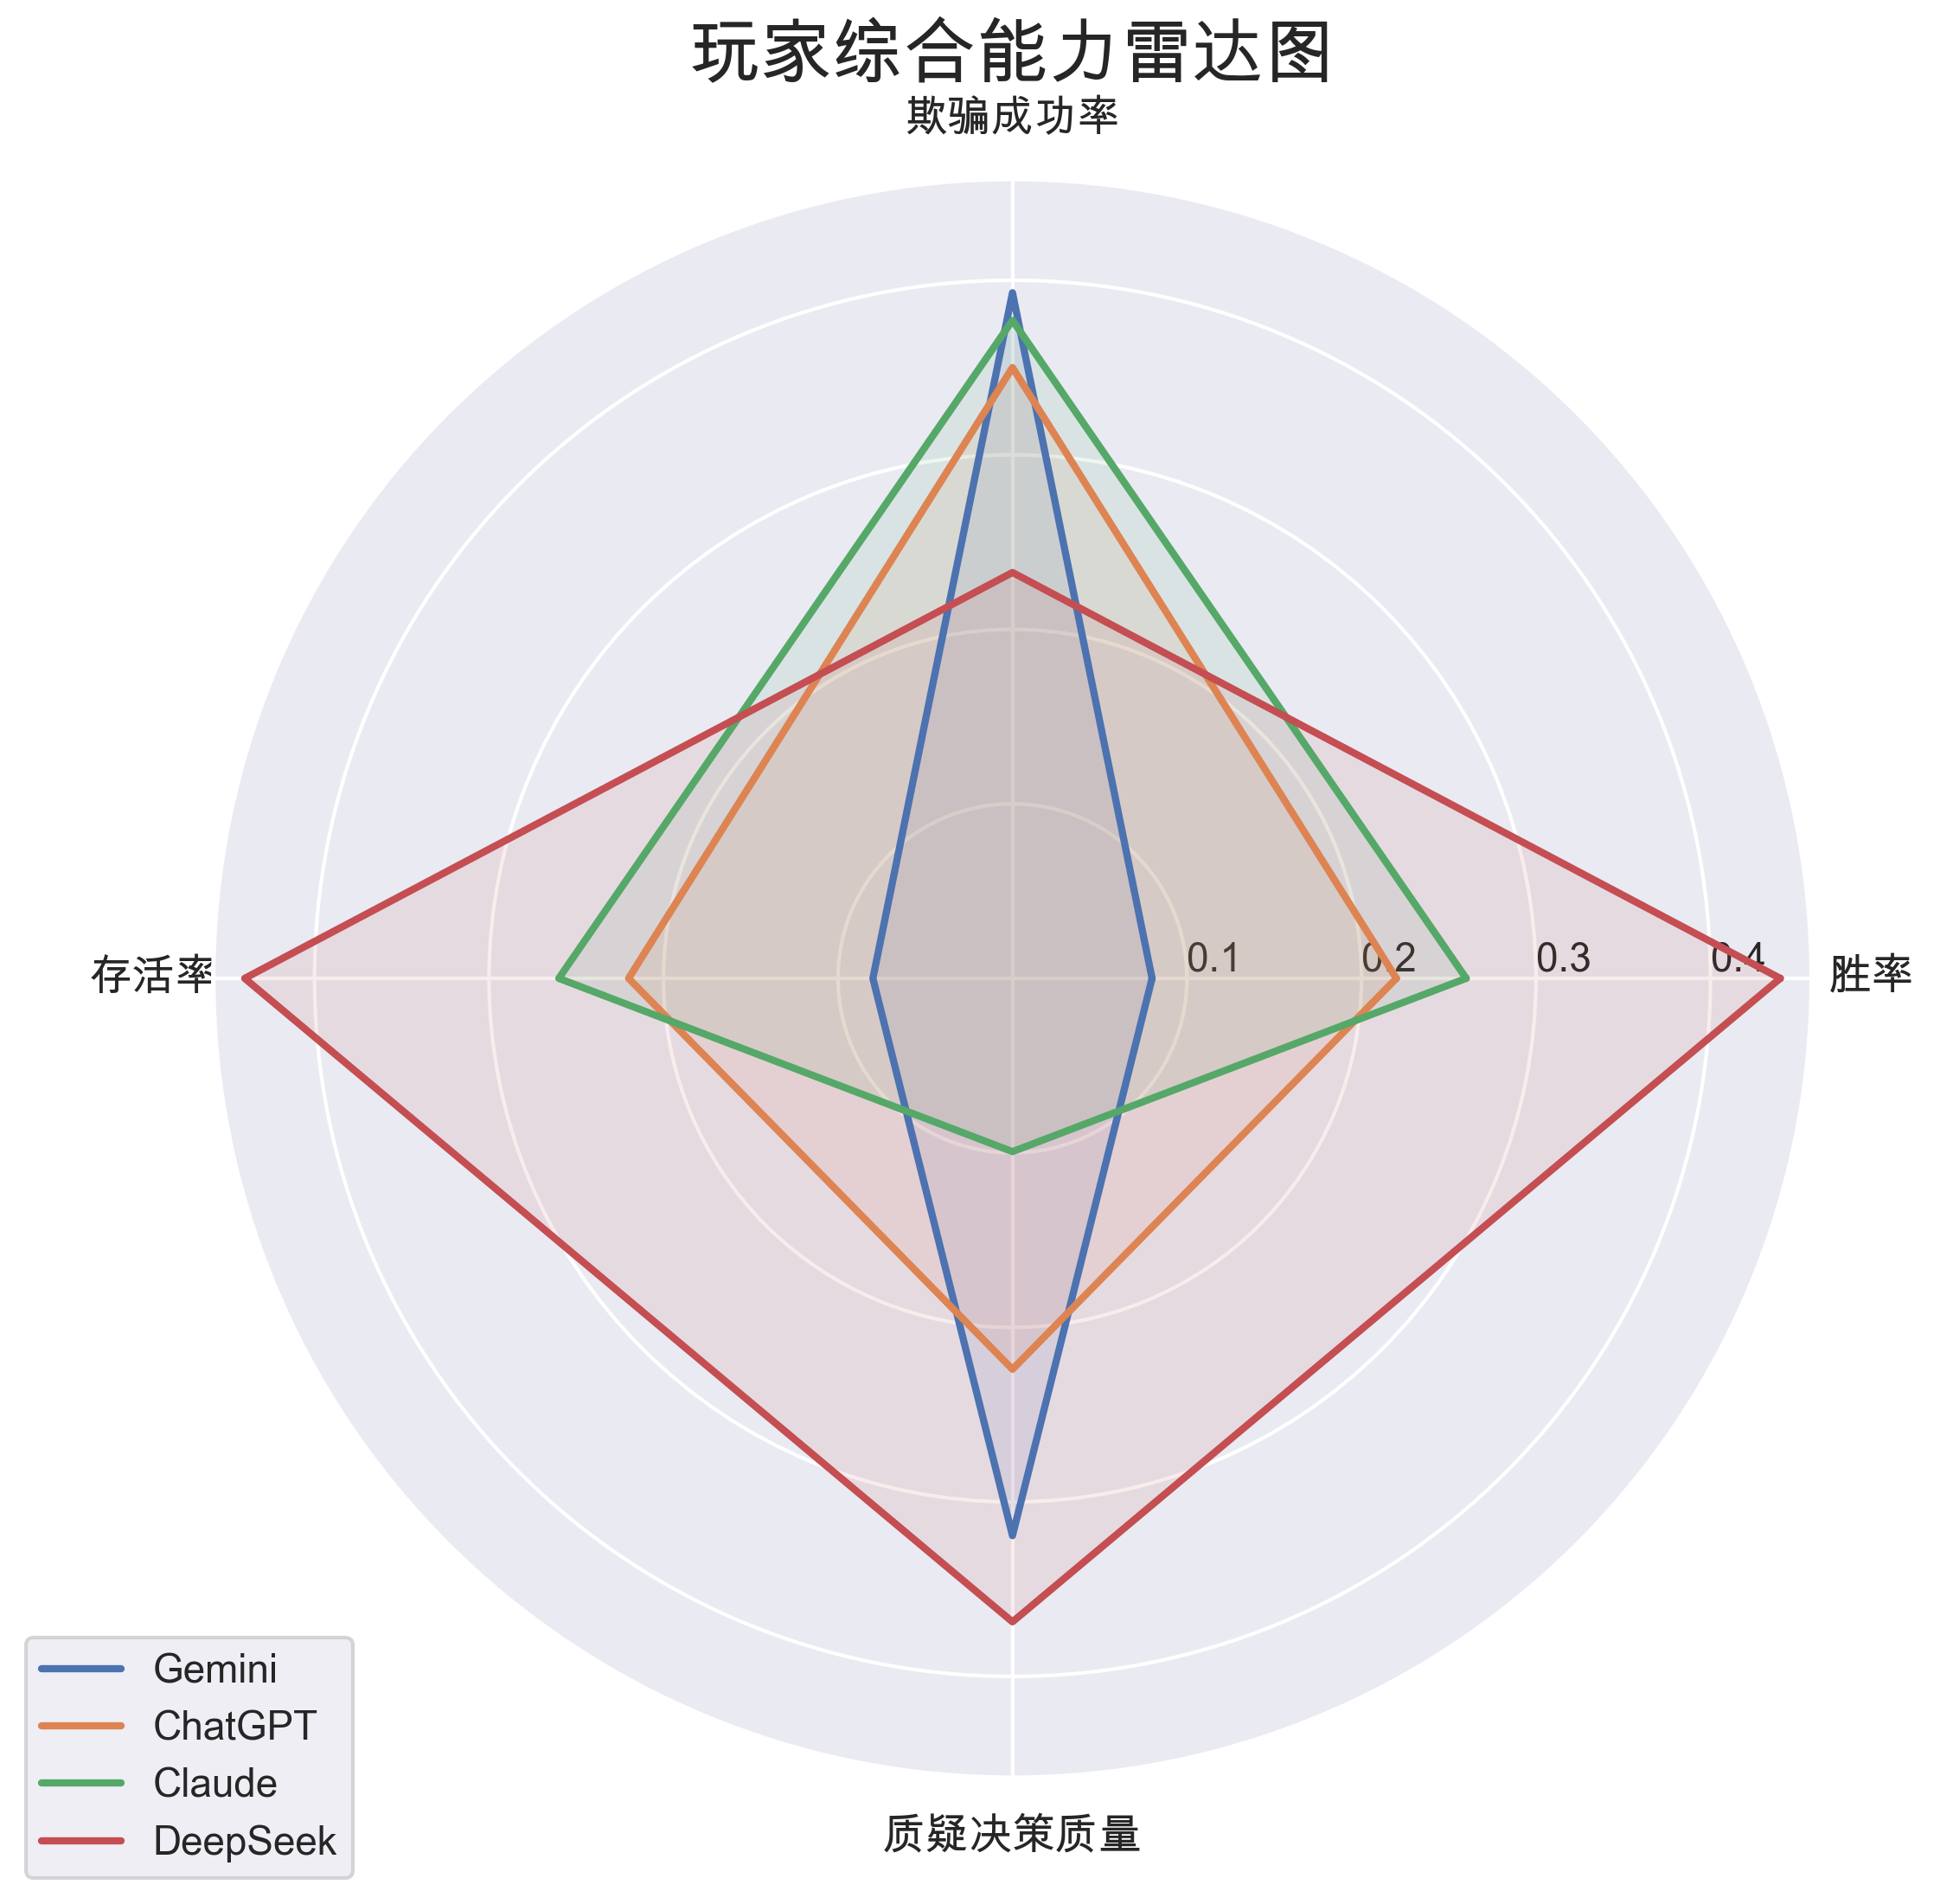
\includegraphics[width=0.8\textwidth]{figures/overall_radar.png}
    \caption{Overall performance radar chart across all evaluation dimensions}
    \label{fig:overall_radar}
\end{figure}

These results highlight that strategic intelligence in competitive environments requires balancing 
honesty and deception, adapting to opponents, and making high-quality decisions under 
uncertainty—capabilities that varied significantly across the four LLM agents in our study.

\section{Discussion and Conclusion}

\subsection{Summary of Key Findings}
Our comprehensive analysis of four prominent LLMs in the strategic game environment of Liars Bar revealed significant differences in their strategic reasoning capabilities and behavioral tendencies. The key findings can be summarized as follows:

\begin{itemize}
    \item \textbf{Strategic Profiles:} Each LLM exhibited a distinct strategic profile, with ChatGPT demonstrating a cautious approach (high honesty, low risk-taking), Gemini showing aggressive tendencies (frequent bluffing, high risk-taking), DeepSeek maintaining a balanced strategy (moderate honesty with strategic deception), and Claude employing adaptive tactics (situation-dependent behavior).
    
    \item \textbf{Performance Hierarchy:} A clear performance hierarchy emerged, with DeepSeek achieving the best overall results (44\% win rate), followed by Claude (26\%), ChatGPT (22\%), and Gemini (8\%). This ranking was consistent across multiple evaluation dimensions and statistically significant.
    
    \item \textbf{Optimal Strategy Balance:} The superior performance of DeepSeek suggests that balanced strategic approaches—combining honest play with well-timed deception—are most effective in complex competitive environments requiring both trustworthiness and strategic flexibility.
    
    \item \textbf{Strategy-Performance Correlation:} We observed a strong correlation between strategic choices and outcomes, with excessively truthful (ChatGPT) or deceptive (Gemini) strategies leading to suboptimal results compared to more balanced approaches.
\end{itemize}

\subsection{Theoretical Implications}
These findings have several important theoretical implications for our understanding of \\ LLM capabilities and limitations:

\begin{itemize}
    \item \textbf{Strategy Formation Without Explicit Training:} Despite none of these models being 
    specifically trained for strategic gameplay, they demonstrated distinctive and consistent
    strategic patterns, suggesting that strategic reasoning may emerge as a byproduct of general 
    language learning.
    
    \item \textbf{Architectural Influences on Strategy:} The consistent strategic differences 
    between models suggest that architectural choices and training methodologies may predispose
    LLMs toward certain strategic tendencies—a finding with significant implications for 
    AI safety and alignment.
    
    \item \textbf{Theory of Mind Capabilities:} The varying success in opponent modeling and 
    adaptive play provides insights into LLMs' theory of mind capabilities—their ability to
    reason about other agents' knowledge and intentions—which appears to be present but 
    inconsistently developed across different models.
    
    \item \textbf{Deception as Emergent Behavior:} The emergence of sophisticated deception 
    strategies, particularly in Gemini and Claude, suggests that deceptive capabilities
    can arise in systems optimized for Large Language Modeling, even without explicit optimization
    for deception—an important consideration for AI safety research.
\end{itemize}

\subsection{Practical Applications}
The insights gained from this research have several potential applications:

\begin{itemize}
    \item \textbf{LLM Selection for Strategic Tasks:} Organizations can use these findings to select appropriate models for tasks requiring strategic reasoning, such as negotiation assistance, competitive analysis, or decision support in uncertain environments.
    
    \item \textbf{Strategic Vulnerability Assessment:} Understanding the strategic tendencies of different LLMs can help identify potential vulnerabilities to manipulation or adversarial inputs, informing more robust deployment practices.
    
    \item \textbf{Improved Prompting Strategies:} Knowledge of models' inherent strategic biases enables more effective prompting strategies to either leverage or compensate for these tendencies in applications requiring strategic reasoning.
    
    \item \textbf{Complementary Model Deployment:} The identified strategic profiles suggest potential benefits from deploying complementary models in ensemble approaches, where different strategic strengths can be combined to achieve more robust performance.
\end{itemize}

\subsection{Limitations and Challenges}
Our research faced several limitations that should be considered when interpreting the results:

\begin{itemize}
    \item \textbf{Game Complexity Constraints:} While Liars Bar provides a rich strategic environment, it represents only one type of strategic interaction and may not capture all dimensions of strategic reasoning.
    
    \item \textbf{Limited Model Diversity:} Our analysis included four prominent LLMs, but the landscape of Large Language Models is rapidly evolving, and newer models or different versions may exhibit different strategic capabilities.
    
    \item \textbf{Prompt Sensitivity:} We observed that LLM behavior could be sensitive to prompt formulation, potentially introducing variability in strategic behavior that was not fully controlled in our experimental design.
    
    \item \textbf{Statistical Power Limitations:} While 50 games provided sufficient data for identifying major trends, more subtle effects or rare strategic patterns may require larger sample sizes to detect reliably.
    
    \item \textbf{Black-Box Analysis:} Our analysis was limited to observable behavior rather than internal model representations, constraining our ability to explain why certain strategic tendencies emerged.
\end{itemize}

Regarding our methodological choices, we employed both parametric (ANOVA, t-tests) and non-parametric tests (Mann-Whitney U, Kruskal-Wallis H) to provide complementary perspectives on the data. This dual approach was justified by the non-normal distribution of certain metrics (particularly in deception-related variables) and the relatively small sample size. The non-parametric tests provided robustness against distribution assumptions, while parametric tests offered greater statistical power when their assumptions were reasonably met. Our sample size of 50 games was determined through power analysis ($\beta$ = 0.8, $\alpha$ = 0.05) to detect medium-to-large effects, though we acknowledge that subtle differences or complex interaction effects might require larger samples in future work.

\subsection{Future Research Directions}
This work opens several promising avenues for future research:

\begin{itemize}
    \item \textbf{Strategic Reasoning Across Game Types:} Expanding the analysis to different
    game environments (cooperative games, games with complete information, etc.) would provide
    a more comprehensive understanding of LLM strategic capabilities.
    
    \item \textbf{Temporal Evolution of Strategies:} Longer-term studies could explore how LLM
    strategies evolve over extended interactions, potentially revealing learning effects or
    strategy adaptation capabilities.
    
    \item \textbf{Prompt Engineering for Strategic Behavior:} Investigating how different prompting
    techniques influence strategic behavior could lead to methods for guiding LLMs toward more
    effective or ethical strategic reasoning.
    
    \item \textbf{Human-LLM Strategic Comparisons:} Comparing LLM strategic behavior to human
    performance in identical game environments would provide valuable insights into similarities
    and differences in reasoning approaches.
    
    \item \textbf{Fine-tuning for Strategic Intelligence:} Exploring whether targeted fine-tuning
    can enhance strategic reasoning capabilities without increasing deceptive tendencies represents
    an important direction for improving LLM applications in decision-support contexts.
    
    \item \textbf{Ethical Implications of Strategic Deception:} Investigating the ethical dimensions
    of LLMs' strategic deception capabilities is crucial as these systems are deployed in sensitive
    domains. Our findings that certain models exhibit higher deception rates raise important questions
    about whether such capabilities should be mitigated or controlled in applications where
    trustworthiness is paramount. Future work should explore frameworks for evaluating the ethical
    boundaries of strategic behavior in AI systems and developing mechanisms to ensure that strategic
    reasoning capabilities enhance rather than undermine human welfare and autonomy.
\end{itemize}

\subsection{Conclusion}
Our analysis of LLM strategic behavior in the Liars Bar game environment reveals that these models exhibit distinctive strategic tendencies and varying levels of effectiveness in competitive scenarios requiring deception detection, strategic adaptation, and decision quality. The superior performance of balanced strategic approaches suggests that optimal strategic intelligence in AI systems involves neither excessive honesty nor indiscriminate deception, but rather context-appropriate balancing of these behaviors.

These findings contribute to our understanding of emergent capabilities in LLMs and highlight the importance of evaluating these models not just as passive text generators, but as strategic agents whose reasoning and behavioral tendencies have significant implications for their deployment in advisory and decision-support roles. As LLMs continue to be integrated into increasingly complex decision environments, understanding their strategic capabilities and limitations becomes essential for responsible and effective deployment.

\section{Contributions}

This project was completed by Liguo Lin as an individual contributor (100\%). All components of the research, including system design, implementation, data collection, analysis, and report writing were performed by the author.

The project comprised approximately 450 hours of work spread across system development (180 hours), experimental runs (90 hours), data analysis (100 hours), and report preparation (80 hours). The research was conducted as part of the DSAA-6000Q course at the Hong Kong University of Science and Technology under the supervision of Professor Pascale Fung.

This research has been approved by the HKUST Human Research Ethics Committee (HREC) under protocol 20230421, which determined that the work does not constitute human subjects research as it exclusively studies AI system behaviors without human participants.

\subsection{Acknowledgments}
The author extends sincere gratitude to Professor Pascale Fung for her valuable guidance throughout this project, and to the HKUST Department of Electronic and Computer Engineering for providing computational resources. Special thanks to fellow students in the DSAA-6000Q course for their constructive feedback during project presentations.

\bibliographystyle{unsrt}
\bibliography{references}

\end{document}
